\documentclass[a4paper, utf8, 11pt, colorlinks]{article} 
\bibliography{localbibliography}
\usepackage{amsmath}
\usepackage[serbian]{babel}
 
\usepackage[OT2,T1]{fontenc}
\usepackage{amssymb}
\newtheorem{definition}{Definicija}
\newtheorem{thm}{Teorema}
\newtheorem{lm}{Lema}
\newtheorem{prop}{Propozicija}
\usepackage{algorithm}
\usepackage{algorithmic}
\usepackage{dot2texi}
%\usetikzlibrary{arrows,shapes}

\newenvironment{proof}{{Dokaz:}}{\hfill$\square$}

% redefinicija nekih konstanti: 
\renewcommand{\figurename}{Slika}
\renewcommand{\tablename}{Tabela}



\usepackage{tikz}
\usetikzlibrary{intersections,calc}
\usepackage{pgfplots} 
\pgfplotsset{compat=newest}
\pgfplotsset{plot coordinates/math parser=false}
\pgfplotsset{
    every non boxed x axis/.style={
        xtick align=center,
        enlarge x limits=true,
        x axis line style={line width=0.8pt, -latex}
},
    every boxed x axis/.style={}, enlargelimits=false
}
\pgfplotsset{
    every non boxed y axis/.style={
        ytick align=center,
        enlarge y limits=true,
        y axis line style={line width=0.8pt, -latex}
},
    every boxed y axis/.style={}, enlargelimits=false
}
\usetikzlibrary{
   arrows.meta,
  intersections,
}


\usetikzlibrary{positioning,shapes.multipart}


\def\textA{$L_0$:\\
	$(x*, y^*)=(2.25, 3.75)$ \\
	$z = 41.25$ \\
	 $z^* \leq 41$
	\vdots
}

\def\textB{$\text{min}\  x_1-2x_2$\\
	subject to\\
	\hspace{1cm}\vdots
	\nodepart{two}
	{\scriptsize $x_1^*=1,x_2^*=2.1667$}
}

\def\textC{$L_1$:\\
	 $x^*=(1.8,  4)$\\
	 $z=41$ \\
	$LB=41$ 
}

\def\textD{$L_2$\\
	$x^*=(3, 3)$ \\
	$z^* = 39 < LB$
}

\def\textE{$L_3$:\\
	podproblem nedopustiv
 }

\def\textF{ $L_4$:\\
    $x^*=(1, 4\frac{4}{9})$ \\
    $z^*=40\frac{5}{9}$ 
}

\def\textG{$L_5$: \\
	$x^*=(1, 4)$ \\
	$z^*=37<LB$
}

\def\textH{$L_6$: \\
	$x^*=(0, 5)$ \\
	$z^*=40<LB$
}

\tikzset{>=stealth,parent node/.style={rectangle split, rectangle split parts=2,align=left,text width=2.5cm,draw,node distance=1cm and 1cm}}
  
  
\usetikzlibrary{positioning}
\newdimen\nodeDist
\nodeDist=25mm
% \ChapterDOI{} %will be filled in at production
\author{
 Marko Đukanović \\ \affiliation{Univerzitet u Banjoj Luci}%\and 
% Noam Chimpsky\affiliation{University of Pluto}\lastand 
% Jane Wilson\affiliation{National Institute for Language}
}
\title{Uvod u Operaciona Istraživanja}

\begin{document}
\maketitle
\newpage
\tableofcontents

\newpage

\section{Uvod}

Operaciona istraživanja su oblast koja pripada matematičkim disciplinama. Ona predstavlja osnovnu disciplinu u menadžmentu, a naziv joj potiče iz njene osnovne uloge, a to je istraživanje  operacija u organizacionim sistemima (logistika, problem raspoređivanja, itd.) gdje je svrha optimizacija (troškova, vremena, $\ldots$). Operaciona istraživanja u osnovi predstavljaju analitički metod rješavanja problema i donošenja odluka koje se primjenjuju u organizaciji raznih sistema. Metodologija metoda najčešće obuhvata razbijanje problema na bazne komponente a potom njihovo rješavanje u definisanim koracima uz pomoć matematičkog aparata. 

Koncept operacionih istraživanja potiče iz Drugog svjetskog rata gdje su vojni planeri razvijali strategiju postavljanja vojske i vojne opreme sa ciljem što veće mobilnosti i efikasnosti. Poslije rata, ove tehnike su primjenjivane u rješavanju mnogih problema u biznisu, socijalnim problemima, i mnogim drugim. 

Proces u operacionom istraživanju se ugrubo može predstaviti sljedećim koracima:
\begin{itemize}
    \item Opisati problem koji rješavamo.
    \item Konstrukcija modela problema koji opisuje taj problem preko varijabli i relacija između njih. 
    \item Korištenje modela za generisanje rješenja problema.
    \item Testiranje svakog od rješenja i analiziranje njihovih  kvaliteta.
    \item Implementacija odabranog rješenja za dati problem. 
\end{itemize}
Glavne karakteristike operacionih istraživanja su
\begin{itemize}
    \item \emph{Optimizacija:} Uloga operacionih istraživanja je dohvatiti najbolje performanse pod unaprijed zadanim resursima (limit u vremenu, memoriji, itd.).  Optimizacija uključuje poređenje i navođenje pretrage prema 
    potencijalno boljim opcijama.
    \item \emph{Simulacija}:  podrazumijeva izgradnju modela problema iz koga se dobijaju rješenja koja se probaju prije nego se implementiraju u realnoj situaciji.
    \item \emph{Vjerovatnoća i statistika}:  podrazumijeva ($i$) upotreba matematičkih algoritama i podataka u smislu otkrivanja korisnih informacija koje služe u davanju pouzdanih predviđanja; ($ii$) testiranja rješenja.
\end{itemize}
 
 Operaciona istraživanja imaju nezamjenjivu ulogu u nizu obasti kao što su problemi raspoređivanja, urbanog planiranja, optimizacije na mrežama i inženjeringu, rutiranja paketa, upravljanja rizicima, upravljanja lancem snabdjevanja i mnogim drugima. 

 Što se tiče   šire slike pojma Operaciona istraživanja, ovo nije niti malo trivijalno opisati. U osnovi, Operacona istraživanja su nauka o tome kako donijeti niz efikasnih odluka. Matematičko programiranje je jedna od najmoćnijih tehnika 
 korištena u Operacionim istrraživanjima do te mjere da  se   ova dva termina ponekad čak poistovjećuju. Treba imati na umu da riječ ``programiranje'' nema standardno značenje na koje smo i navikli, već ono označava optimizaciju. Operaciona istraživanja rješavaju probleme iz prakse (nazovimo ih biznis problemi) koje ljudima štede novac i vrijeme. Ovi problemi mogu biti raznoliki i po pravilu izgledaju nbez povezanosti jedan sa drugim. Gledajući šire, osnovica im je uvijek ista, donošenje niza odluka da bi se došlo do cilja na što efikasniji način.  %Diskretna optimizacija 

  Put od učenja o problemu kojeg klijent prezentuje do pronalaska rješenja može biti jako izazovno. Ovaj proces rješavanja se može podijeliti u četiri osnovna nivoa apstrakcije:
  \begin{enumerate}
      \item Biznis problemi
      \item Generički problemi 
      \item Paradigma modelovanja
      \item Algoritamska rješenja
  \end{enumerate}
  
 Pod \emph{biznis problemima} ne uzimamo  samo probleme iz domena ekonomije. Tu su svi problemi koji imaju primjenu u stvarnom svijetu. Pojam ``biznis'' više odgovara tome da problem nema svoju matematičku formulaciju, nego je manje formalno definisan, kroz jezički (deskriptivan) opis.  Najčešće, ovi problemi proizilaze iz problem u industriji i kao takvi se i opisuju. Primjer takvog problema je u problemu raspoređivanja medicinskog osoblja u (tri) smjene sa uslovima poput toga da svaki radnik mora da odradi 40 sati sedmično ili da niti jedan radnik ne smije da radi više od dvije noćne smjene u toku sedmice. Sljedeći korak 
 je formalno definisanje problema, dakle, spuštanje (opisa) problema na niži nivo apstrakcije. U praksi, ovo ide iterativno. Ovaj proces se povezuje sa terminom \emph{Generički problemi}. 

Pri konceptualizaciji Operacionih istraživanja na početku nije bilo jakog matematičkog formalizma. Matematičari su prepoznali da se većina biznis problema može  mapira u generičke familije problema nižeg nivoa. Ovom mapiranju je posvećeno dosta vremena, da bi se na kraju završilo sa nekoliko standardnih generičkih klasa. U praksi, najveći dio vremena se provodi u konvertovanju biznis problema u jedan od poznatih generičkih problema. Nakon toga, rješavanje problema je manje-više standardna procedura. Generički problemi operacionih istraživanja su dovoljno koncizni da se mogu predstaviti preko matematičke notacije. Međutim, u svrhu boljeg razumijevanja u praksi se koriste jezici modelovanja koji su na višem nivou apstrakcije od njih; tako npr. problemi raspoređivanja se obično opisuju preko resursa, aktivnosti i uslova redosljeda. 

\emph{Paradigma modelovanja}. Kod generičkih operacinih problema koji su definisani jezikom višeg nivoa, notacija je najčešće vezana uz problem koji se razmatra.
Kao primjer, resursi i aktivnosti nisu nešto što se može definisati u, recimo, problemu trgovačkog putnika. U osnovi, svaki od ovih generičkih problema se mogu opisati nekom od paradigmi modelovanja. Paradigma modelovanja predstavlja skup pravila koja omogućuju da predstavimo probleme višeg nivoa koristeći strukture nižeg nivoa, kao što su, recimo, matrice. Kada se primjenjuje ova paradigma, problem se izražava koristeći matematičku notaciju ili algebarski jezik modelovanja (eng. \emph{Algebraic Modelling Language} (AML)) koji konvertuje matematičku notaciju u matrice koje su prosljeđene sljedećem nivou \emph{algoritamska rješenja} koja generišu rješenja. Najpoznatije paradigme modelovanja su sljedeće: Linearno, Cjelobrojno i Mješovito-cjelobrojno programiranje. Postoje još neki modeli poput Modelovanje ograničenjima (Constraint Programming) i mrežno modelovanje (Networks models). 

\emph{Algoritamska rješenja}. Algoritam je procedura ili konačan niz instrukcija čijim izvršavanjem možemo riješiti problem. Neki algoritmi su opšti, kao što su sortiranje ili pretrage i primjenjivi su u raznim poljima kompjuterskih nauka, dok su drugi vezani uz specifične probleme. Algoritmi pretrage su izuzetni važni u rješavanju problema operacionih istraživanja. Među njima se izdvajaju ``Branch \& X''-tip algoritama koji rješavaju Cjelobrojna, Mješovito-cjelobrojne probleme kao i probleme zasnovane na modelovanju ograničenjima. Specifično, među ove algoritme spadaju Branch \& Bound (za rješavanje problema cjelobrojnog programiranja), Branch \& Cut, Branch \& Price (tj. metod generisanja kolona), itd.

Među programskim paradigmama koje su značajne u operacionim istraživanjima takođe izdvajamo i dinamičko programiranje. Ova familija algoritama rješava probleme tako što eksploatiše optimalnu pod-strukturu problema. U prevodu, ako problem može da bude riješen koristeći identične zadatke, riješimo jedan od zadataka i smjestimo rješenje u tabelu (memorišemo). Kada u sljedećem momentu   rješavanja problema naiđemo na isti podproblem, jednostavno ga ne rješavamo ponovo, već rješenje pročitamo iz tabele. Ova programska paradigma ima značajnu ulogu u rješavanju grafovskih problema. Jedan od najpoznatijih je Bellman-Ford-ov algoritam, nazvan po izumitelju ove paradigme, Ričardu Belmanu. 
U praksi problemi mogu biti prilično teški za egzaktno rješavanje, a potrebno je naći brzo rješenje. Za to nam služe pohlepni algoritmi. Oni obično ne mogu 
garantovati optimalnost pri svom prekidu, ali su oni po svojoj prirodi jako brzi. Najpoznatiji takav algoritam je Dajkstrin algoritam za problem pronalaska najkraćeg puta koji pri nekim karakteristikama grafa čak nalazi optimalno rješenje. 

\begin{figure}
    \centering
    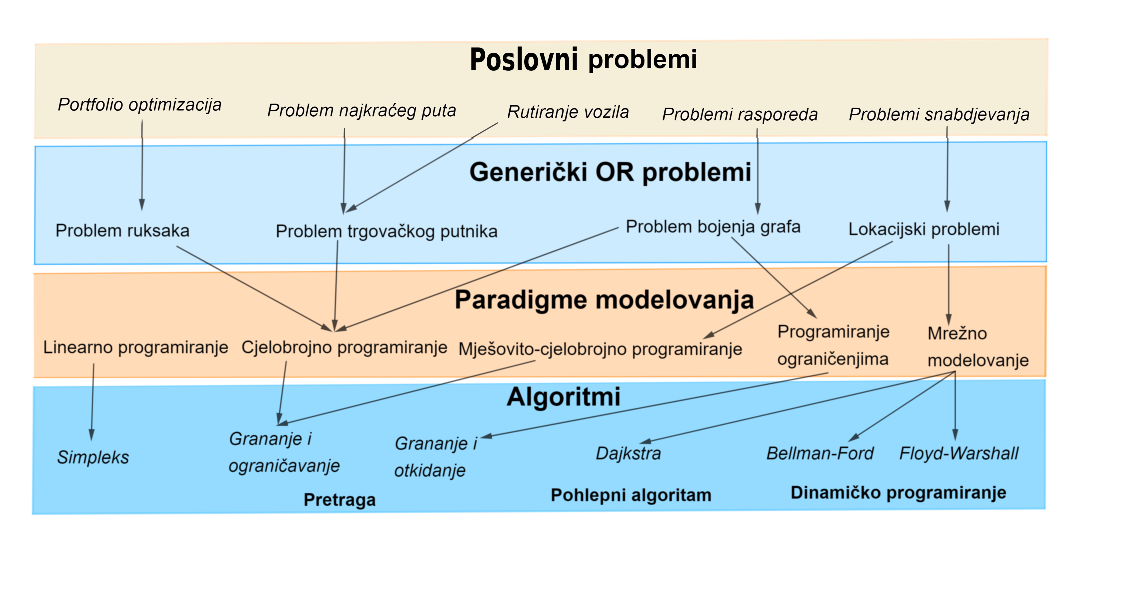
\includegraphics[width=300, height=230pt]{overview.eps}
    \caption{Četiri nivoa apstrakcije pri rješavanu problema operacionih istraživanja.}
    \label{fig:OR_four_levels}
\end{figure}
%https://towardsdatascience.com/the-big-picture-of-operations-research-8652d5153aad


U nastavku knjige ćemo objasniti u detalje svaki od nivoa apstrakcije u operacionim istraživanjima kao i svaku od paradigmi modelovanja i najznačajnije algoritame za rješavanje. Odnos između sva četiri nivoa apstrakcije su data na Slici~\ref{fig:OR_four_levels}. 
 Na kraju knjige će biti riječi o generalnom rješavaču koji je alatka za rješavanje problema u operacionim istraživanjima. 
 \\
 \newpage
 
 
\section{Principi Modelovanja u Operacionim Istraživanjima}
Prije svega, kada govorimo o pojmu Operaciona istraživanja, uvijek ćemo od sada koristiti skraćenicu OR (eng. operational research). 
U ovoj glavi ćemo objasniti   glavne faze tipičnog OR istraživanja koje se tiče komercijalne svrhe. Faze OR možemo sumirati u sljedeće (preklapajuće) faze: 
\begin{itemize}
    \item Definisanje problema i skupljanje relevantnih podataka.
    \item Formulisanje matematičkog modela datog problema.
    \item Razvoj računalne procedure koja će vratiti rješenja datog problema na osnovu modela.
    \item Testiranje modela i po potrebi njegova poboljšanja.
    \item Priprema za primjenu modela kako je definisano od strane menadžmenta koji finansira sistem.
    \item Implementacija rješenja.
\end{itemize}
 Svaka od ovih faza će biti opisana u nastavku.
 
 \subsection{Definisanje problema i skupljanje relevantnih podataka}
 
Većina praktičnih problema sa kojima se susreću OR timovi su u početku opisani na jako neprecizan način. Prema tome, prvi zadatak podrazumijeva dobro definisati  cilj problema (engl. objectives), uslovi pod kojim je rješenje validno,  vremenski limit za donošenje odluka, moguće alternativne akcije, itd. Proces definisanja problema na dobar načij je krucijalan jer uveliko utiče na relevantnost zaključaka istraživanja. Izvlačenje pravog odgovora iz pogrešne postavke problema je praksa koja ne vodi ispravnom rješenju.  

Prvo bitna čunjenica je da OR tim ne radi sam, već radi na principu savjetovanja. Članovi tima koji su zaduženi za formulisanje problema savjetuju se sa menadžmentom gdje tim zatim izvodi detaljne tehničke analize u vezi problema i prezentuje preporuke za rješenje menadžmentu (osobi koja je ključna u donošenju odluka). 
Najčešće, izvještaj menadžmentu će sadržati brojne alternative koje u osnovi odgovaraju različitim uslovima ili različitim  vrijednostima parametara izmjerene od strane menadžmenta (kao na primjer, vaganje između cijene i dobiti). Menadžment zatim vrednuje istraživanje i prijedloge, uzimajući u obzir  niz faktora te donosi odluku baziranu na najboljoj procjeni. Ono što je bitno je da OR tim bude približno sličnog mišljenja kao i menadžment. Utvrđivanje odgovarajućih ciljeva je veoma važno za ispravno definisanje problema.  Za to je potrebno imati osobu iz menadžmenta koja je donosilac odluka za sistem u razvoju i onda pristupiti inidividualnom razmišljanju realizacije pojedinačnih ciljeva.

OR istraživanje po ``defaultu'' traži ona rješenja koja su optimalna prije nego suboptimalna koja su optimalna samo za određenu komponentu procesa koji zahtjeva izradu sistema (tj. za problem koji se nastoji definisati). Prema tome, ciljevi koji su formulisani trebali bi biti oni koji traže optimalna rješenja čitave organizacije i procesa koji se optimizuje. Međutim, obično to nije trivijalno, pa se problem svodi na razmatranje dijela inicijalnog (opisanog) problema jer bi analiza postala glomazna ako bi zadani ciljevi bili pregeneralni. Umjesto toga, ciljevi bi trebalo biti specifični 
koliko god je to moguće, ali pri tome da obuhvate glavne ciljeve donosioca odluka a pri tome zadržavaju razuman stepen konzistentnosti sa osnovim ciljevima organizacije. 

Kada su u pitanju profitne organizacije, jedan od mogućih pristupa zaobilaženja problema pod-optimizacije je koristiti dugoročnu maksimizaciju profita. Riječ dugoročno ukazuje da ovaj cilj pruža fleksibilnost u razmatranju aktivnosti koje ne donose dobit momentalno 
(npr. istraživački i razvojni projekti), ali moraju se uključiti na kraju kako bi donijeli profit. Ovakav cilj je   dovoljno specifičan, a ipak izgleda dovoljno širok da obuhvati osnovni cilj profitnih organizacija, a to je zarada na kraju krajeva. U stvari, svi drugi legitimni ciljevi ovakvih organizacija mogu prevesti se prevesti u gore pomenuti. U praksi, profitne organizacije rijetko koriste ovaj pristup. U osnivi, velik broj profitnih organizacija adaptira zadovoljavajući profit sa drugim ciljevima mjesto fokusiranja maksimizacije dugoročne zarade. Neki od tih ciljeva su: izgradnja stabilnog profita, proširivanje tržišta, zadržavanje stabilnosti cijena, povećanje uticaja kompanije, povećanje raznolikosti proizvoda, itd. 
Dalje, postoje dodatna razmatranja poput društvenih odgovornosti koje nisu direktno motivisane profitom.  

Postoji nekoliko strana kojih se direktno tiču poslovi firme: (1) vlasnici (dioničari, itd.), koji žele profit;   (2) zaposlenici koji žele stalno zaposlenje te razumne plate; (3) kupci koji žele proizvod razumne kvalitete po razumnoj cijeni;
(4) dobavljači, koji žele integritet i razumnu prodajnu cijenu proizvoda; i
(5) Vlada, koja želi plaćanje poreza te razmjenu dobara. Svih pet strana daje doprinos firmi. Stoga, dok je glavna odgovornost menadžmenta profit (što u konačnici koristi svim stranama), napomenimo da se moraju sagledati i širi društveni uticaj ovakvog procesa. 
 
 OR timovi obično provode veliku količinu vremena prikupljajući relevantne podatke o problemu. Mnogo podataka je potrebno prikupiti kako bi se došlo do tačnog razumijevanja problema i dolaska do potrebnih ulaznih podataka za matematički model koji se konstruiše u narednoj fazi.  Često mnogi    podaci nisu dostupni, bilo zbog toga što informacije nikada nisu sačuvane ili su zastarile ili su sačuvane u pogrešnom obliku.   OR tim će obično   traži pomoć ključnih pojedinaca u organizaciji kako bi pronašli sve podatke značajne za projekat. Međutim, mnogi podaci mogu biti prilično ``neprecizni", tj. grube procjene zasnovane samo na iskustvenim pretpostavkama tima. OR tim će provesti značajnu količinu vremena pokušavajući poboljšati
preciznost podataka, a zatim nastaviti proces sa najboljim mogućim resursima skoji su prikupljeni. 

\textbf{Primjer.}  OR studija je urađena za policijsku upravu San Francisca na razvoj kompjuterizovanog sistema za optimalno raspoređivanje i postavljanje patrolnih službenika. U procjeni odgovarajućih ciljeva ove studije, identifikovani su sljedeći ciljevi:
\begin{enumerate}
    \item  Održavati visok nivo sigurnosti građana.
    \item  Održavati visok nivo zadovoljstva u policiji.
     \item Minimizirati troškove operacija.
\end{enumerate}
Da bi se postigao prvi cilj, policijska uprava i gradska vlada zajednički su radili u uspostavljanju željenog nivoa zaštite.  Matematički model koji je razvijen je nametnuo uslov da će se postići potreban nivo zaštite preko funkcije cilja. U samom modelu je nametnut uslov o ravnopravno uravnotežnim radnim satima među policajcima u cilju postizanja drugog cilja. Treći cilj je ugrađen usvajanjem dugoročnog cilja smanjenja broja policajaca potrebnih za postizanje prva dva cilja. 

\subsection{Proces Formulisanja Matematičkog Modela}

Nakon što se definiše problem odlučivanja, sljedeća faza je preformulisati takav problema u oblik prikladan za analizu. Konvencionalni OR pristup se sastoji u konstrukciju matematičkog modela koji pokriva suštinu problema. Prije nego objasnimo kako konstruisati takav model, recimo nešto o modelima u opštem slučaju, a posebno o matematičkim modelima.

Modeli (idealizovani prikazi) su sastavni su dio svakodnevnog života. Uobičajeni 
primjeri uključuju model aviona, portreta, globusa i tako dalje. Slično tome, modeli igraju
važnu ulogu u nauci i poslovanju, što uključuje modele atoma, modele 
genetskih struktura, matematičke jednačine koje opisuju fizikalne zakone kretanja, grafikoni, itd. Takvi modeli
su od neprocjenjive važnosti za apstraktno poimanje suštine predmeta istraživanja, ukazivanje na međusobnu interakciju pojava i olakšavanja analize. 

Matematički modeli mogu da budu izraženi preko matematičkih simbola kao što je poznata formula $F=ma$ iz fizike. Slično, matematički model biznis problema   
se sastoji od sistema jednačina i matematičkih izraza koji opisuju osnov problema. Dakle, postiji $n$ mjerljivih odluka koje treba da budu donesene, predstavljene pomoću nepoznatih (varijable) $x_1,\ldots, x_n$ čije vrijednosti treba da budu izračunate.  Odgovarajuća mjera učinka (profita) je onda izražena preko matematičkih funkcija nepoznatih koje odgovaraju  odlukama (primjer, $3x_1 + 5x_2 + x_3$). Ovaj funkcija se naziva ciljna (objektivna) funkcija. Restrikcije  vrijednosti promjenjivih su takođe izražene matematički, preko jednakosti ili nejednakosti (npr. $x_1 + x_2 + x_3 \leq 1$).  Ovakvi matematički izrazi za restrikcije se nazivaju ograničenja (eng. constraints). Konstante u ograničenjima te u ciljnoj funkciji se nazivaju parametri modela. Prema tome, matematički model 
podrazumijeva izabrati vrijednosti varijabli (odluka) tako da se maksimizuje vrijednost funkcije cilja u odnosu na određena ograničenja. Takvi modeli sa manjim varijacijama karakterišu  modele koji su korišteni u OR polju. 
Određivanje odgovarajućih vrijednosti koje se dodijeljuju parametrima modela je kritični dio procesa konstrukcije modela.
Za razliku od problema u udžbenicima, u kojima su ove vrijednosti unaprijed date, njihovo određivanje parametara u stvarnim problemima zahtijeva prikupljanje relevantnih podataka. Kao što je objašnjeno u prethodnoj sekciji,  prikupljanje tačnih podataka je veoma izazovno. Stoga dodijeljena vrijednost parametara predstavlja često grubu procjenu. Zbog nesigurnosti u  stvarnoj vrijednosti parametara, važno je analizirati kako se rješenje koje je izvedeno iz modela mijenja pri malim promjenama vrijednosti parametara. 
 Problemi iz prakse obično nemaju samo jedan ``pravi'' model.  U praski je često   dva ili više potpuno različitih modela odgovaraju jednom problemu. 
Ovo je stvar razvoja modela koji je iterativni proces koji proizilazi iz rezultata testiranja i potrebe za boljim modelom.  
 U nastavku ćemo vidjeti brojne primjere matematičkih modela. Jedna posebno važna vrsta koju proučavamo u sljedećih nekoliko poglavlja
je model linearnog programiranja, gdje su ciljna funkcija i ograničenja   sve linearne funkcije. 
Matematički modeli imaju prednost u odnosu na jezički opis problema -- problem se opisuje mnogo sažetije. Na taj način cjelokupna struktura problema je razumljivija i otkrivanje važnih uzročno-posljedičnih veza u samom problemu je dosta lakše. Takođe, matematički
model čini premosnicu za korišćenje snažnih matematičkih tehnika i računara u
analizi problema. Zapravo, softveri za rješavanje raznih tipova modela su  u današnje vrijeme  široko dostupni (Cplex, Gurobi, Lindo itd.). 

  Postoje i zamke na koje treba paziti kada koristimo matematičke modele. Kako je model ``apstraktna idealizacija problema'', aproksimacije i pojednostavljivanje pretpostavki uglavnom su neophodni ako je model izvršiv (tj. sposoban za rješavanje problema). Stoga se mora paziti da model ostane valjan prikaz problema nakon pojednostavljenja. To znači da 
  sve što je potrebno jest da postoji velika korelacija između onoga što model predviđa i onoga što bi se zapravo dobilo u stvarnom svijetu. Da bi se utvrdilo je li ovaj zahtjev zadovoljen, potrebno je izvršiti znatna ispitivanja i posljedične izmjene u inicijalnom modelu, što je tema narednih podsekcija. U osnovi, provjera valjanosti modela zapravo se provodi tijekom faze izrade modela što pomaže u vođenju konstrukcije matematičkog modela do njegove krajnje verzije. 
  
 U razvoju modela, dobar pristup je započeti s vrlo jednostavnom verzijom te   krenuti sa evolucionim načinom prema složenijim modelima koji će dobro odražavati složenost stvarnog problema. Ovaj proces obogaćivanja modela nastavlja se sve dok je model rješiv. Osnovni kompromis kojeg držimo na oku je između preciznosti modela i izvršivosti modela.
  Ključni korak u razvoju OR modela je konstrukcija ciljne funkcije.
To podrazumijeva razvijanje kvantitativne mjere uspješnosti u odnosu na svaki   krajnji cilj koji je identifikovan tokom definisanja problema.
Ako postoji više ciljeva, njihove se mjere obično transformišu
i kombinuju u jednu složenu mjeru.  Ukupna mjera može biti nešto opipljivo (npr. dobit) koja odgovara višem cilju
organizacije ili može biti apstraktna.  Nakon što se razvije cjelokupna mjera,  ciljna se funkcija izražava kao matematička funkcija čiji su argumenti varijable odluke. \vspace{0.3cm}\\
% primjer preuzet iz: http://www.mathos.unios.hr/~mdjumic/uploads/diplomski/ČOR03.pdf
\textbf{Primjer.}  Uzmimo jednog proizvođa\v ca negaziranih pi\'ca. On pravi dvije vrste soka: Spring i Orandž od sastojaka $A$ i $B$ te vode. Da bi se napravilo 100$l$ Springa potrebno je 3$l$
sastojka $A$ i 8l sastojka $B$, a za Orandž je potrebno 6l sastojka $A$ i 4l sastojka $B$. Sto litara Springa nosi zaradu od 100kn, a 100$l$ Orandža zaradu od 125kn. Proizvođa\v c u skladi\v stu
ima na raspolaganju 30$l$ sastojka $A$ i 44l sastojka $B.$ Napravljene sokove sipa u ba\v cve. Za
Spring ima ba\v cvu u koju stane 500$l$ teku\' cine, a za Orandž ba\v cvu kapaciteta 400$l$. Na kraju dana dolazi preprodava\v c koji kupuje sok. Cilj proizvođa\v ca sokova je napraviti koliko god
mo\v ze soka, uzimaju\' ci u obzir dana ograni\v cenja, kako bi maksimizirao svoj profit. Drugim
rije\v cima, treba napraviti plan proizvodnje koji \' ce maksimizirati profit.

Model za ovakav problem bi išao ovako:
\begin{itemize}
    \item 
Varijable odluke: $x_1$ i $x_2$ koje označavaju koliko litara soka Springa i koliko litara soka Orandž proizvođač treba da napravi.  
\item Funkcija cilja: $f(x_1, x_2) = c_1x_1 + c_2 x_2$, gdje su $c_1 = 100$ i  $c_2 = 125$ koeficijenti. Funkciju $f$ treba maksimizovati. \\
\item Ograničenja: $0 \leq x_1 \leq 5, 0 \leq x_2 \leq 4$,   $3 x_1 + 6 x_2 \leq 30$, $8 x_1 + 4 x_2 \leq 44.$
\end{itemize}

\subsection{Izvođenje Rješenja iz Modela}

Nakon formulacije matematičkog modela za problem, sljedeća faza u OR studiji je razvoj postupka (algoritma) za
izvođenje rješenja na osnovu konstruisanog modela. To je ponekad relativno jednostavan korak u kojem jedan od standardnih algoritama biva pušten na računaru pomoću jednog od   dostupnih softverskih paketa (Cplex, Gurobi, itd.). Međutim, pravi posao dolazi u sljedećim koracima, koji uključuje postoptimalnu
analizu koju objašnjavamo kasnije. Veći dio ove knjige posvećujemo metodama koje pronalaze rješenja iz modela, tako da nećemo dužiti previše u vezi toga. Više ćemo govoriti o prirodi   rješenja.  Uobičajena tema u OR polju je potraga za optimalnim (najboljim) rješenjem. Razvijeni su mnogi postupci, koji će biti predstavljeni u nastavku, za pronala\-ženje optimalnih rješenja iz nekih vrsta modela. Treba imati na umu da su ta rješenja optimalna samo za dati model. Kako model ne mora modelovati stvarni problem, već njegovu idealizovanu varijantu, ne postoji garancija da će se optimalno rješenje tog modela pokazati najboljim mogućim rješenjem za stvarni problem koji se razmatra. Međutim, ako je
model dobro formulisan i testiran, rezultirajuće rješenje trebalo bi biti prihvatljiva zamjena rješenja stvarnog problema. U praksi često ``dovoljno dobro'' rješenje je prihvatljivije nego tražiti optimalno. Najčešće se prvo postavi lista zahtjeva koje dati model treba da ispuni i rješenje koje zadovoljava te uslove najčešće se i uzme kao dobro. OR timovi pokušavaju unijeti što je moguće više ``vrhunske znanosti''  (tj. ispunjavanje nalazaska optimuma) u proces donošenja odluka. Međutim,  uslov da se u razumnom vremenskom roku dođe do niza odlika koje vode ka rješenju koje je zadovoljavajuće najčešće prednjači u odnosu na nalazak optimuma. Tim bi također trebao razmotriti troškove procesa razvoja modela, a zatim
pokušati maksimizovati korist u oba smijera. OR timovi povremeno koriste samo heurističke pristupe rješavanju problema (tj. intuitivno dizajnirane postupke kojima se ne garantiraju optimalno rješenje) kako bi pronašli razumno suboptimalno rješenje. To je najčešće slučaj kada je trošak pronalaska  optimalnog rješenja  modela vrlo velik. Posljednjih godina postignut je velik napredak u razvoju efiksanih heurističkih postupaka (uključujući tzv.
metaheuristike), pa njihova upotreba u ovom polju iz dana u dan  dobija sve više na značaju.  

Nađeno optimalno/podoptimalno rješenje za konstruisani model može biti daleko od idealnog za stvarni problem, pa su potrebne dodatne analize. Stoga je analiza postoptimalnosti (analiza provedena nakon pronalaska (pod)optimalnog rješenja) vrlo važan dio   OR studija.  Ova analiza se ponekad naziva i šta--ako analiza, jer uključuje postavljanje pitanja o tome što bi bilo sa optimalnim rješenjem ako se uvedu različite pretpostavke što implicira dodavanje novih ograničenja u postojeći model. Ova pitanja često postavlja menadžment koji će donijeti konačne odluke u vezi procesa dodavanja uslova, a ne tim koji radi na modelovanju.

Pojava softvera koji rade sa proračunskim tablicama (Excel) igraju središnju ulogu u provođenju analize postoptimalnosti. Jedna od velikih prednosti ovakvih softvera je jednostavnost u korišćenju, gdje se lako dobija analiza šta se događa sa optimalnim rješenjem kada se naprave promjene na modelu.  Ovakva eksperimentisanja sa promjenama u modelu mogu biti od velike pomoći u razumijevanju ponašanja samog modela i uvjeravanja u njegovu valjanost.  Analiza postoptimalnosti dijelom  uključuje provođenje analize osjetljivosti radi utvrđivanja koji parametri modela su najkritičniji (``osjetljivi parametri'') u određivanju rješenja. Uobičajena definicija osjetljivog parametra je sljedeća:

Za matematički model osjetljivi parametri modela su parametri čije se vrijednosti ne mogu mijenjati bez promjene optimalnog rješenja. Prepoznavanje osjetljivih parametara važno je jer se time nalaze parametri čija se vrijednost mora dodijeliti sa posebnom pažnjom kako bi se izbjeglo narušavanje rezultata modela.

Da napomenemo, vrijednost koja se parametru obično dodjeljuje samo je procjena neke veličine
(npr. jedinična dobit) čija će tačna vrijednost postati poznata tek nakon što se rješenje primijeni na problem. Stoga, nakon
što se identifikuju osjetljivi parametri, posebna pažnja se posvećuje bližoj procjeni svakog parametra te  raspona njihovih mogućih vrijednosti.  U nekim slučajevima, određeni parametri modela predstavljaju interesne odluke (npr. dodjele resursa). Ako je to slučaj, često postoji određena fleksibilnost u vrijednostima koje se dodjeljuju ovakvim parametrima u smislu da se neke vrijednosti povećavaju  smanjenjem drugih. Postoptimalna analiza uključuje istraživanje takvih kompromisa. Analiza postoptimalnosti takođe uključuje dobivanje niza rješenja koji aktivira niz poboljšanja u modelu i konvergenciju prema idealnijem modelu. Postupak poboljšanja modela se nastavlja sve dok    poboljšanja u sljedećim rješenjima ne postanu premala da bi se nastavilo sa ovakvim iterativnim procesom.   Alternativna rješenja (rješenja koja su optimalna za jedan od nekoliko probližnih modela) se takođe mogu predstaviti menadžmentu za konačan odabir. 

%\textbf{Primjer.}  Posmatrajmo OR studiju o nacionalnom upravljanja vodama.


\subsection{Testiranje Modela}
Razvoj velikih matematičkih modela je analogan razvoju velikih softvera. Kad se dovrši prva verzija softvera, ona neizbježno sadrži mnogo bugova. Stoga, pristupa se testiranju kako bi se pokušalo pronaći i
ispraviti što više bugova. Na kraju, nakon niza iteracija poboljšanja programa, programeri zaključuju da trenutni program sada
daje generalno valjane rezultate. Obično, neke manje pogreške nesumnjivo ostaju skrivene u programu, a možda nikada neće biti otkrivene. Glavne pogreške su manje-više uklonjene da se program sada može pouzdano koristiti.  Slično tome, prva verzija matematičkog modela neizbježno sadrži mnoge
nedostatke. Neki relevantni faktori ili međusobni odnosi ne budu   ugrađeni
u model, a neki parametri ne budu pravilno procijenjeni. Sve to
je neizbježno, s obzirom na potencijalne probleme u komunikaciji kao i razumijevanju svih aspekata problema te poteškoća pri prikupljanju pouzdanih podataka. Stoga, prije nego što upotrijebimo model, on se mora  temeljno testirati kako bismo mogli  identifikovati 
i ispraviti što više njegovih ndostataka. Na kraju, nakon dugog niza poboljšanih
modela, OR tim koji radi na modelu zaključuje da trenutni model sada daje razumno valjane rezultate.  Iako neki manji nedostaci nesumnjivo ostaju skriveni u modelu (a možda nikada neće ni biti otkriveni), glavni nedostaci su uklonjeni tako da se može tvrditi da je model pouzdan. Ovaj postupak ispitivanja i poboljšanja modela radi povećanja njegove valjanosti se naziva \emph{validacija modela}. 

Budući da OR tim može provesti mjesece na izradu svih detalja modela, lako je izgubiti suštinu zbog detalja. Stoga, nakon što su detalji uključeni u 
početnu verziju modela, dobar način za početak provjere valjanosti je ponovni pogled na cjelokupni model kako bi se provjerilo da li ima  očiglednih pogrešaka ili propusta. Poželjno je da grupa koja radi ovaj pregled uključi barem jednog pojedinca koji nije učestvovao u konstrukciji modela. Preispitivanje definicije
problema i poređenje sa modelom mogu pomoći u otkrivanju nekih pogrešaka. Također je korisno da su svi matematički izrazi dimenzionalno konzistentni.  Ponekad se  dodatni uvid u valjanost modela dobija i 
mijenjanjem vrijednosti parametara i / ili varijabli odluke i provjerom da li se  izlaz iz modela ponaša na očekivan način. To se često otkriva kada se parametrima ili varijablama dodjeljuju ekstremne vrijednosti u blizini njihovih maksimuma ili minimuma. 
 
  Sistematski pristup ispitivanju modela podrazumijeva upotreba retrospektivnog testa. Ovaj test uključuje upotrebu istorijskih podataka koja prati konstrukciju modela, a zatim utvrđuje koliko bi dobro funkcionisao model i rezultirajuće rješenje 
ako bi rješenje bilo korišteno u praksi.  Ovaj pristup može ukazati na dijelove na kojima model ima nedostatke što zahtijeva njegove izmjene. 
S druge strane, nedostatak retrospektivnog ispitivanja je taj što koristi iste podatke kao i oni koji vode ka formulaciju modela. Ključno je pitanje da li prošlost zaista reprezentuje budućnost. %Da bi se zaobišao   nedostatak retrospektivnog testiranja, ponekad je korisno privremeno nastaviti sa statusom quo. To će dati nove podatke koji nisu bili dostupni kada  je
  %model konstruiran. 
  Važno je još dokumentovati postupke koji se koriste u testiranju valjanosti modela. Ovo može  povećati povjerenje u model za buduće korisnike. Takođe, ako se u budućnosti pojave pitanja u vezi sa modelom, ova će dokumentacija biti korisna u dijagnosticiranju problema. 

\begin{comment}
 \textbf{Primjer.}  Primjer se odnosi na OR studiju provedenu   za IBM kako bi se integrisala nacionalna mreža zaliha rezervnih dijelova radi poboljšanja servisne podrške za IBM-ove kupce.

Ovom studijom je dobijen  novi inventarni sistem koji je poboljšao korisničku uslugu kroz koju se uštedilo dodatnih 20 milijuna USD po godini kroz poboljšanu operativnu efikasnost. Posebno zanimljiv aspekt faze provjere validnosti modela ove studije bio je način na koji su  budući korisnici inventarnog sistema ugrađeni u postupak ispitivanja. Prvo su odabrani predstavnici koji su činili korisnički tim čija je uloga bila  savjetovati OR tim. Nakon što je razvijena preliminarna verzija novog sistema izvršeno je njgovo testiranje. Opsežne povratne informacije korisničkog tima dovele su do glavnih poboljšanja u predloženom sistemu.  
\end{comment}

 \subsection{Priprema za Primjenu Modela}
 Ako želimo da model bude iskorišten više puta, sljedeći  korak je instaliranje dobro dokumentovanog sistema za primjenu modela po propisima naručioca (menadžmenta). Ovaj sistem uključuje inplementaciju samog modela, postupak dobijanja rješenja (uključujući analizu postoptimalnosti) operativne postupke za izvođenje, itd. %Tada, čak i kad se osoblje mijenja, sistem se može pozvati na regularnoj bazi da se ponudi određeno numeričko rješenje
 Baze podataka i informacioni sistem za upravljanje treba da pružiti ažuran unos za model svaki put pri korištenju; u tom je slučaju potrebno obezbijediti interfejs. Nakon što se na model primijeni postupak rješavanja (drugi program), dodatni   programi mogu automatski pokrenuti implementaciju rezultata da bi korisnici to mogli odmah da primijene u realnoj situaciji. U drugim se slučajevima instalira interaktivni računarski sistem  nazvan sistemi za podršku odlučivanju koji pomaže menadžerima da koriste podatke i modele kako bi podržali (a ne zamijenili) njihovo donošenje odluka po potrebi. Drugi program može generirati menadžerske izvještaje (na jeziku upravljanja) koja tumače izlazne podatke modela i njegove implikacije na primjenu, koji se indirektno koristi u implementiraciji rješenja.  U velikim OR studijama potrebno je nekoliko mjeseci (ili duže) za razvoj, testiranje i instaliranje ovakvog računarskog sistema. Dio ovog napora uključuje razvoj i izvođenje postupka održavanja sistema  tokom njegove buduće upotrebe. Kao se uslovi mijenjaju tokom vremena, potrebno je  modifikovati sistem, uključujući i sam model, u skladu sa tim uslovima.  

Sljedeći primjer nam opisuje sistem u IBM-u za kontrolu usluga i zaliha rezervi da bi se dobio osjećaj o kompleksnosti ovakvih sistema.  

\textbf{Primjer.}
%OR studija  za IBM predstavljena na kraju prošle sekcije je primjer   velikog sistema koji integriše model.
 Sistem nazvan \emph{Optimizer} pruža optimalnu kontrolu usluga i zaliha rezervnih dijelova u cijeloj IBM-ovoj mreži za distribuciju dijelova u SAD-u, koja uključuje dva središnja
automatizovana skladišta, deseci terenskih distribucijskih centara i postaja za dijelove te nekoliko hiljada vanjskih (povezanih) lokacija. Inventar dijelova koji se održava u ovoj mreži se procijenjuje u milijardama dolara. \emph{Optimizer} se sastoji od četiri glavna modula. Modul sistema predviđanja sadrži nekoliko programa za procjenu stope kvara pojedinih vrsta dijelova. Modul sistema za dostavljanje podataka sastoji se od otprilike 100 programa koji    obrađuju
preko 15 Gb podataka kako bi se osigurali ulazni podaci za model. Sistem odlučivanja potom rješava model koji traje i  sedmicu dana kako bi se optimizovala kontrola zaliha. Četvrti modul uključuje šest programa koji integriraju \emph{Optimizer} u IBM-ov sistem upravljanja zalihama dijelova (PIMS). %PIMS je sofisticirani informacijski i kontrolni sustav koji sadrži milijune redaka koda 
\subsection{Implementacija}
Nakon što se razvije sistem za primjenu modela, posljednja faza OR studije je primjena ovog sistema kako ga je uprava (koja naručuje razvoj sistema) propisala. Ova je faza ključna jer se ovdje ``ubiru plodovi rada''. Stoga je važno da OR tim  sudjeluje u  lanisiranju ove faze, kako bi se osiguralo da se rješenja modela precizno prevedu u operativni postupak i kako bi se ispravili svi nedostaci u rješenjima koja se otkriju. Uspjeh faze implementacije uvelike ovisi o podršci i vrha uprave i operativnog menadžmenta. Mnogo je vjerojatnije da će OR tim dobiti potporu ako je dobro informisao upravu i poticao  njeno vođstvo tijekom studija na aktivno učešće. Dobra komunikacija pomaže da studija postignu ono što je uprava željela te takođe potiče njihovu potporu u izvršenje čitavog projekta.  Faza provođenja uključuje nekoliko koraka. Prvo, OR tim daje operativnom rukovodstvu opis novog sistema koji treba da bude usvojen. Dalje, ove dvije strane dijele odgovornost za razvijanje koraka potrebnih za pokretanje ovog sistema. Operativno rukovodstvo zatim posmatra uključeno osoblje kojima daje detaljna uputstva za korištenje sistema, čime počinje proces primjene. Ako se sistem uspješno uvede, novi sistem se može koristiti u godinama koje dolaze. Imajući to na umu, OR tim nadgleda iskustva korisnika sistem i nastoji utvrditi koje izmjene bi trebalo da se urade na sistemu u budućnosti u cilju lakšeg korištenja.  Tokom vremena u kojem se koristi novi sistem, važno je i dalje dobijati povratne informacije o funkcionisanju sistema te da li su pretpostavke o modelu i dalje zadovoljene. Kada se pojave značajna odstupanja od originalnih pretpostavki modela, model treba ponovno pogledati radi utvrđivanja treba li se u sistemu izvršiti bilo kakve izmjene. Nakon završetka projekta, potrebno je da OR tim dokumentuje svoju metodologiju dovoljno jasno i precizno kako bi se čitav posao mogao ponoviti. Repliciranje bi trebalo
biti dio profesionalnog etičkog kodeksa projektovanja (informacionih) sistema. %Ovo je stanje osobito važno kada se proučavaju kontroverzna pitanja javne politike. 

\textbf{Primjer.} Vratimo se na naš IBM projekat pomenut u prethodnim sekcijama.  Tri su se glavna faktora pokazala posebno važnim za uspješan završetak projekta. Kao što je raspravljano u prethodnim poglavljima, 
prvo je   uključivanje korisničkog tima i (operativnog rukovodstva) kao savjetnika OR tima tokom trajanja cijelog projekta. U vrijeme faze implementacije, operativno rukovodstvo imalo je snažan  uticaj te pobornici instaliranja \emph{Optimizer}-a u  funkcionalna područja poslovanja IBM-a. Drugi faktor uspjeha bio je vrlo široka povratna informacija korisnika sistema gdje su identifikovane problematične tačke u sistemu koje su  trebale biti ispravljene prije potpune implementacije. 
Treći faktor je bio taj da je novi sustav postupno uvođen fazu po fazu, uz pažljivo testiranje u svakoj fazi, kako bi se veće pogreške mogle ukloniti prije nego što je sistem   pušten na  nacionalnoj (i operativnoj) razini.  
\vspace{0.5cm}

Ostatak ove knjige je fokusiran prvenstveno na konstruisanje i rješavanje matematičkih modela. Sa ovim poglavljem  smo  pokušali objasniti da konstrukcija modela složenih problema ne sadrži samo ova dva koraka, već su oni samo dio cjelokupnog OR procesa. Treba imati na umu da su druge faze vrlo važne za provođenje uspješnog OR istraživanja. Predlažemo da se nakon izučavanja načina rješavanja modela, čitalac vrati na ovo poglavlje u cilju što jasnije slike razvoja potpunog OR istraživanja zasnovano na kompleksnim procesima u praksi.  OR zahtijeva značajnu količinu domišljatosti i inovativnosti, pa ne postoji standardni postupak kojeg bi se trebali pridržavati OR timovi koji razvijaju sisteme zasnovane na OR. %Prethodni opis može da se promatra kao model koji otprilike pokazuje koliko je uspješan ILI se provode studije. 
\newpage

\section{Linearno Programiranje} 
   
Razvoj linearnog programiranja se smatra među najvažnijim naučnim dostignu\-ćima XX vijeka. Njegov uticaj od 1950. je ogroman u nauci i industriji. Danas je to standardni alat koji je uštedio milione dolara ogromnom broju firmi u raznim zemljama svijeta  Napisani su deseci udžbenika
o linearnom programiranju i objavljeno stotine radova koji opisuju važne primjene ove paradigme.  Linearno programiranje koristi matematički model za opisivanje problema. 
Pridjev linearni znači da su   sve matematičke funkcije u ovom modelu linearne funkcije. Riječ programiranje se ne odnosi na računarsko programiranje; nego je to sinonim za planiranje i optimizaciju. Dakle, linearno programiranje uključuje planiranje aktivnosti u cilju postizanja optimalnog rezultata, tj. rezultata koji najbolje postiže navedeni cilj (prema matematičkom modelu) među svim izvedivim alternativama.  Za rješavanje problema linearnog programiranja dostupan je izuzetno efikasan metod rješavanja, nazvan \emph{simpleks metod}. On rješava probleme ogromnih veličina te je on jedan od razloga ogromnog utjecaja linearnog programiranja posljednjih nekoliko decenija.

\textbf{Primjer}. WYNDOR--GLASS CO projekat: Proizvodi visokokvalitetne staklene proizvode, uključujući prozore i staklena vrata. Postoje tri pogona. Aluminijski okviri i okovi izrađuju se u pogonu 1, drveni okviri izrađuju se u pogonu 2, a pogon 3 proizvodi staklo i sastavlja proizvode.
Zbog pada zarade, rukovodstvo firme je odlučio je obnoviti liniju proizvoda tvrtke. Neprofitabilni proizvodi se ukidaju, oslobađajući proizvodne kapacitete za lansiranje dva nova proizvoda sa velikim prodajnim potencijalom:
\begin{itemize}
    \item Proizvod 1: Staklena vrata od 8 $m$ sa aluminijskim okvirom.
    \item Proizvod 2: Dvostruko obješen drveni okvir s okvirom visine 4 $m$.
\end{itemize}
Uslovi i zahtjevi proizvodnje su sljedeći:
\begin{itemize}
    \item Proizvod 1 zahtijeva   korištenje proizvodnih kapaciteta u postrojenjima 1 i 3, ali nijedan u pogonu 2. 
    \item Proizvod 2 treba   postrojenja 2 i 3. 
\end{itemize}
    Rukovodstvo je zaključio da bi kompanija mogla prodati sve proizvode koje bi mogla proizvesti u postrojenjima. Međutim, budući da se oba proizvoda koriste proizvodni kapacitet u pogonu 3, nije jasno koja bi kombinacija dva proizvoda bila najisplativija. Stoga je formiran OR tim za proučavanje ovog pitanja, te davanja adekvatnog odgovora.

OR tim započinje razgovor sa rukovodstvom kako bi se utvrdili ciljevi ovog istraživanja. Te su rasprave dovele do   sljedeće definicije (idealizovanog) problema:
\begin{itemize}
    \item Utvrditi  stope proizvodnje  ova dva proizvoda kako bi se maksimalizirala ukupna dobit, podložno ograničenjima koja nameću   proizvodni kapaciteti dostupni u tri pogona. Svaki će se proizvod proizvoditi u serijama od po 20, tako da se stopa proizvodnje definiše kao broj serija proizvedenih na nivou jedne sedmice. Dopuštena je bilo koja kombinacija stope proizvodnje koja zadovoljava   ograničenja, uključujući proizvodnju 0 komada prvog proizvoda i što  više   drugog. 
\end{itemize}

 OR tim je identifikovao podatke koje je trebalo prikupiti: 
($i$) Broj radnih sati u sedmici dostupan u svakom pogonu za nove proizvode.  
($ii$) Broj radnih sati korištenih u svakom pogonu za svaku proizvedenu seriju svakog novog proizvoda.
($iii$) Dobit po proizvedenoj seriji svakog novog proizvoda. Dobit po proizvedenoj seriji odabrana je kao odgovarajuća mjera nakon što je tim zaključio da će inkrementalna dobit   svake dodatne proizvedene serije   približno konstantna bez obzira na ukupan broj proizvedenih serija.

Budući da značajniji troškovi za pokretanje
 proizvodnje i promovisanju novih proizvoda neće postojati, ukupna dobit je približno jednaka dobiti po proizvedenoj seriji puta broj serija.  

Nakon ovoga, trebalo je procijeniti konstante u modelu. Ovaj proces je tekao u komunikaciji između organizacije i OR tima. 
Za dobivanje razumnih procjena, pomoć ključnog osoblja u raznim jedinicama firme je bila važna. Osoblje u proizvodnom odjelu dalo je podatke za ($i$). Razvoj procjena za ($ii$) zahtijeva analizu proizvodnih inženjera uključenih u dizajniranje proizvodnih procesa novih proizvoda. Analizirajući podatke o resursima inženjera i marketinškog odjela,  razvijena procjena za treću kategoriju. Tabela~\ref{tab:procjene-1} daje te procjene. 

\begin{table}[!ht]
    \centering
    \begin{tabular}{c|c c | c}
    \      &      \multicolumn{2}{l}{Vrijeme proizvodnje serije ($h$)}    & \  \\ \hline
    \      &      \multicolumn{2}{l}{Proizvod}                      & \  \\ 
    Pogon  &  1    &      2                                 & Vrijeme za proizvodnju po sedm. ($h$) \\ \hline 
           1 & 1  &  0 &  4  \\
           2 & 0  &  2 &  12  \\ 
           3 & 3  &  2 &  18  \\ \hline
           Profit po seriji & 3000 & 5000 & \  \\
           \hline
    \end{tabular}
    \caption{Procjene konstanti modela.}
    \label{tab:procjene-1}
\end{table}

Konstruišimo sada model. Uvedimo varijablu $x_1$ za broj serija proizvoda 1 proizvedenog na sedmičnom nivou, te $x_2$ broj serija proizvoda 2 proizvedenog na sedmičnom nivou. Funkcija profita je jednaka $f(x_1, x_2) = 3 x_1 + 5 x_2$ pod uslovima
\begin{itemize}
    \item $x_1, x_2 \geq 0$
    \item  $x_1 \leq 4, 2 x_2 \leq 12$
    \item $3 x_1 + 2 x_2 \leq 18$
\end{itemize}
%https://www.desmos.com/calculator
\subsection{Rješenje grafičkom metodom}
 Problem iz prethodne sekcije se veoma malen jer sadrži samo dvije varijable odluke i samim tim sve alternative mogu biti predstavljene u dvije dimenzije. U tom slučaju, pri njegovom rješavanju može se koristiti grafička metoda. Ovaj postupak uključuje konstrukciju dvodimenzionalnog osnog sistema sa osama $x_1$ i $x_2$.  Prvi korak je identifikovati vrijednosti ($x_1$, $x_2$) koje su dopuštene ograničenjima. Njih drugačije zovemo dopustivim rješenjima. To se radi crtanjem svake od 
linija koja se graniči sa rasponom dopuštenih vrijednosti ograničenja. Ograničimo prostor sastavljen od svih 6 uslova, što rezultira slikom~\ref{fig:fig1}.  Rezultujući region dopustivih rješenja $(x_1, x_2)$ se naziva dopustivi region. Posljednji je korak odabrati tačku u ovom regionu  koja maksimizira vrijednost $f = 3x_1 + 5x_2$. 

%) The resulting region of permissible values of (x1, x2), called the feasible region,
\begin{figure}
    \centering
    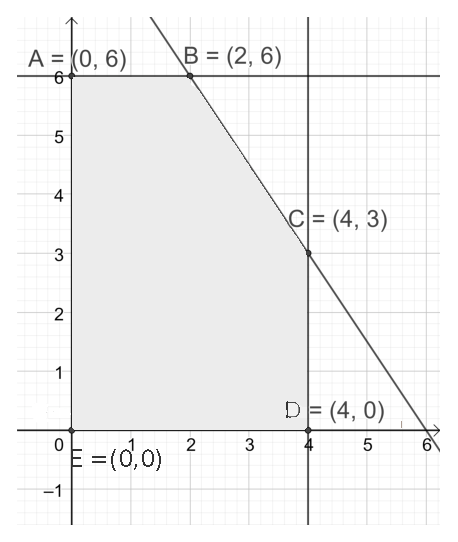
\includegraphics[width=150pt,height=150pt]{fig1.eps}
    \caption{Dopustiv region.}
    \label{fig:fig1}
\end{figure}
Pogledajmo sada grafike $3x_1 + 5 x_2 = c$, za $c \in \{10,20, 36\}$, kao na Slici~\ref{fig:fig2}. Jasno se vidi da prava $f = 36$ prolazi kroz tačku (vrh) regiona $(2,6)$ koja je dopustiva. Dakle, jasno je da je $(2, 6)$ rješenje problema i da niti jedna druga funkcija $f=c, c > 36$ ne presijeca dopustiv region. 

Ovaj se postupak često naziva \emph{grafičkom metodom za linearno programiranje}. Ona se može koristiti za rješavanje bilo kojeg problema linearnog programiranja s dvije varijable. Uz znatan trud, moguće je proširiti ovu metodu na problem sa tri varijable, što je krajnji domet grafičke metode. Za uopšten slučaj se koristi  simpleks metoda o kojoj će biti riječi u narednim sekcijama.

\subsection{Standardna Forma Linearnog Programiranja}

\begin{figure}[!ht]
    \centering
    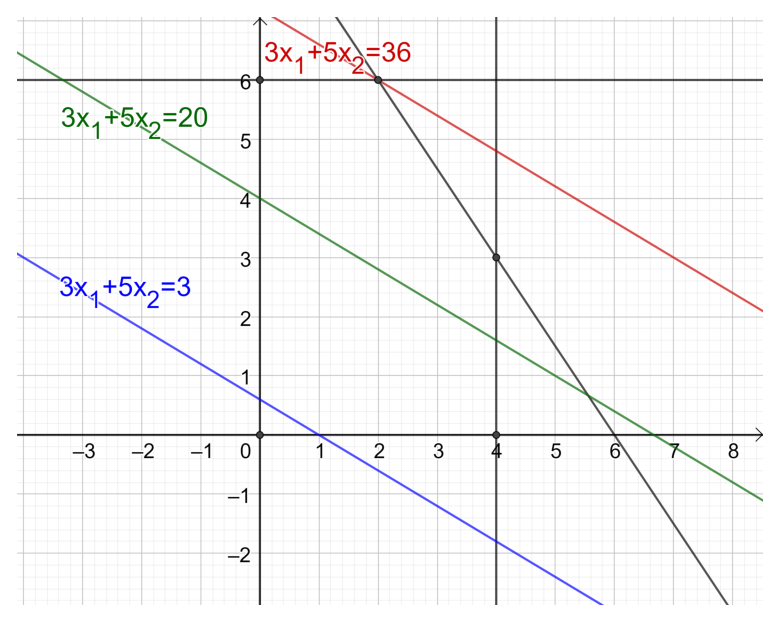
\includegraphics[width=160pt, height=160pt]{fig2.eps}
    \caption{Dodavanje $f = c$ i nalazak optimuma transliranjem po dopustivom regionu.}
    \label{fig:fig2}
\end{figure}

U ovoj sekciji govorimo o opštoj formi modela linearnog programiranja. 
Ključni pojmovi su resursi i aktivnosti, gdje recimo imamo $m$ vrsta resursa i $n$ aktivnosti koji se razmatraju. Standardni resursi su novac, oprema, vrste mašina, itd. Aktivnosti uljučuju ulaganja u određene projekte, oglašavanja, dostavljanje robe iz jednog u drugo mjesto, itd. 
 Najčešći tip primjene linearnog programiranja uključuje dodjelu resursa određenim aktivnostima. Dostupna količina svakog resursa je ograničena, pa aktivnost mora biti pažljivo raspoređena odgovarajućem resursu.  Utvrđivanje ove raspodjele uključuje odabir nivoa aktivnosti za koje se postiže
najbolja moguća vrijednost ukupne mjere učinka. 

U nastavku navodimo notaciju koja se najčešće koriste u formiranju generalnog oblika modela linearnog programiranja:

\begin{itemize}
    \item $f$: funkcija cilja (dobiti) 
    \item $x_j$: količina aktivnosti $j$ ($j = 1,\ldots,n$);
    \item $c_j$: povećanje u profitu ako se količna aktivnosti $j$ podigne za jediničnu vrijednost;
    \item $b_i$: ukupna količina resursa $i$ ($i=1,\ldots,m$) koja je dozvoljena za lociranje aktivnosti;
    \item $a_{ij}$: količina resursa $i$ koja se konzumira od strane jedinične vrijednosti aktivnosti $j$.
\end{itemize}
Prema tome, matematički modeli problema linearnog programiranja ima sljedeću postavku:

\begin{align} 
      &f = c_1 x_1 + \cdots + c_n x_n \rightarrow \max \label{form:LP-1}\\
      & s.t. \nonumber \\
      & a_{11}x_1 + a_{12} x_{12} + \cdots + a_{1n}x_n \leq b_1 \label{form:LP-2} \\
      &\ldots \nonumber \\
      & a_{m1}x_1 + a_{12} x_{m2} + \cdots + a_{mn}x_n \leq b_m \label{form:LP-3} \\
      & x_i \geq 0, i=1,\ldots,n.\label{form:LP-4}
\end{align}

Postavka (\ref{form:LP-1})--(\ref{form:LP-4}) se još naziva i \emph{standardna forma} problema linearnog programiranja. Funkcija (\ref{form:LP-1}) se naziva funkcija cilja koju je potrebno maksimizovati pod uslovima (\ref{form:LP-2})--(\ref{form:LP-3}) koji se nazivaju \emph{funkcionalna ograničenja}, dok (\ref{form:LP-4}) se nazivaju \emph{nenegativna ograničenja}. 

Kompaktiniji oblik standardne forme je dat sa:
\begin{align}
    & f = c^T x \rightarrow \max \label{eq:LP-o1}\\
    &  A x \leq b \label{eq:LP-c1} \\
    & x \geq 0 \label{eq:LP-c2}.
\end{align}

gdje je $A \in \mathbb{R}^{m \times n}$, $x \in \mathbb{R}^n$ i $b \in \mathbb{R}^{m \times 1}$. Imajte na umu da ograničenja (\ref{eq:LP-c1}) mogu da imaju i oblike:
\begin{itemize}
    \item $Ax \geq b$;
    \item $Ax = b$;
    \item neke od varijabli $x_i=0$.
\end{itemize}
Bilo koji problem koji koristi neke od prethodna tri ograničenja predstavlja i dalje problem linearnog programiranja. U nastavku pratimo sljedeću terminologiju u vezi linearnog programiranja (LP):
\begin{itemize}
    \item \emph{Rješenje} u standardnom matematičkom značenju najčešće označava krajnje rješenje   (u LP-u bi to bilo najbolje rješenje). Međutim, u rješavanju problema LP-a to  nije slučaj. Bilo koja specifikacija vrijednosti varijabli  $(x_1,\ldots, x_n)$ se smatra rješenjem bez obzira da li je riječ o željenom rješenju ili čak onom rješenju koje ne zadovoljava kriterijume. U zavisnosti od toga, rješenja u  možemo podijeliti na:
    \begin{itemize}
        \item \emph{dopustiva rješenja} (eng. \emph{feasible solution}) -- podrazumijevanju ona rješenja koja zadovoljavaju sva ograničenja u modelu;
        \item \emph{nedopustiva rješenja} (eng. \emph{infreasible solution}) -- ona rješenja koja ne zadovoljavaju barem jedno od ograničenja u model. 
    \end{itemize}
  \item \emph{Dopustivi region}: označava skup svih rješenja koja su dopustiva. Ovo je prostor koji pretražujemo u svrhu pronalaska najboljeg rješenja modela. Takođe, može se desiti da problem nema niti jedno dopustivo rješenje. Kažemo da je tah problem \emph{nedopustiv}. 
  \item \emph{Optimalno rješenje} je ono rješenje iz dopustivog skupa za koje je funkcija cilja najveća (pod pretpostavkom da maksimizujemo). Ova vrijednost ne mora biti jedinstvena, pogledati sliku~\ref{fig:multi_solution} gdje je dopustiv region isti kao u primjeru sa slike~\ref{fig:fig1}, dok je funkcija cilja data sa $f = 3x_1 + 2 x_2$.  
 \end{itemize}
 
 \begin{figure}
     \centering
     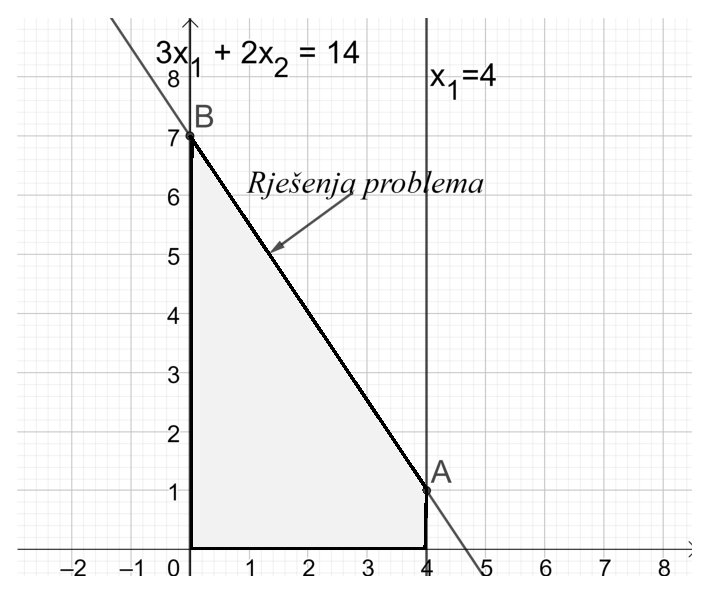
\includegraphics[width=160pt, height=160pt]{fig3.eps}
     \caption{LP sa više od jednog optimalnog rješenja.}
     \label{fig:multi_solution}
 \end{figure}
 
 Za razliku od nedopustivog problema, može se desiti i druga situacija, da je problem neograničen. U tom slučaju vrijednosti (jedne od) varijabli se mogu povećavati tako da funkcija cilja teži ka beskonačno, tj. nije ograničena odozgo nekom vrijednošći. Za taj problem kažemo da je \emph{neograničen} problem. Primjer takvog problema možemo vidjeti na slici~\ref{fig:unbounded_solution}, gdje je potrebno maksimizovati funkciju $f = 3 x_1 + x_2$, pod uslovima $0\leq x_1 \leq 4$, te $x_2 \geq 0$. Kao što se može vidjeti, što se više povećava vrijednost varijable $x_2$ to funkcija $f$ više raste. Ako bi $x_2$ bilo $\infty$, to bi i funkcija $f$ bila neograničena ($f = \infty$).
 
  \begin{figure}
     \centering
     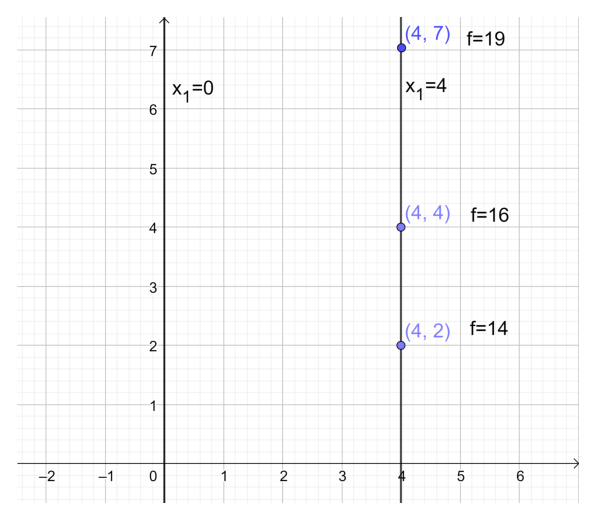
\includegraphics[width=160pt, height=160pt]{fig4.eps}
     \caption{Primjer LP-a koji je neograničen.}
     \label{fig:unbounded_solution}
 \end{figure}
 
Uvedimo pojam \emph{ekstremalnih tačaka}, koje igraju bitnu ulogu u simpleks metodi, koja rješava LP u generalnom obliku. Za rješenje $x$ kažemo da je \emph{ekstremna tačka} ako se nalazi u vrhu dopustivog regiona (u presjeku ivica dopustivog regiona).  Postoji neraskidiva veza između ovih tačaka i optimalnog rješenja LP-a. Ove veze ćemo dokazati u nastavku ove knjige. Uglavnom, vrijede sljedeće činjenice. 
Razmotrimo bilo koji problem LP-a sa dopustivim rješenjima i ograničenom dopustivom regijom. Problem mora posjedovati barem jednu tačku u vrhu i barem jedno optimalno rješenje. Nadalje, najbolja tačka u vrhu dopustivog regiona mora biti optimalno rješenje. Dakle, ako problem ima tačno jedno optimalno rješenje, to mora biti tačka u vrhu. Ako problem ima više optimalnih rješenja, barem dva moraju biti rješenja koja su tačke u vrhu dopustivog regiona.

\textit{Napomena.} Imajte na umu da (optimalno) rješenje LP-a ne mora da bude cjelobrojno. Budući da svaka varijabla odluke predstavlja nivo odgovarajuće aktivnosti, pretpostavlja se da se aktivnosti mogu izvoditi na razlomljenim nivoima (aktivnost  se ne dijeli samo na diskretne dijelove), na osnovu nenegativnih ograničenja.  

\subsection{Problemi Modelovani preko Linearnog Programiranja}

\emph{Problem optimalne prehrane.} 

Pretpostavimo da su nam na raspolaganju namirnice $N_1, \ldots, N_n$. Cijena namirnice $N_j$ po jedinici je $c_j, j = 1, \ldots, n$. U namirnicama su prisutni nutritivni elementi $e_j,j=1,\ldots,m$ pri čemu
u namirnici $N_j$ ima $a_{ij}$ nutritivnog elementa $e_i$, $i = 1, \ldots, n$, $j = 1, \ldots, m$. Svaka osoba u toku dana mora unijeti barem $b_i$
jedinica nutritivnog elementa $e_i$. Potrebno je formulisati
sljedeći problem: 

\emph{Koliko treba konzumirati pojedine namirnice da bi se zadovoljila dnevna
potreba za nutritivnim elementima, a da se pri tome minimizira cijena prehrane?}
 
 \emph{Rješenje.}  Uvedimo prvo varijable $x_j \geq 0$ za količinu konzumirane hrane namirnice $N_j$, $j = 1, \ldots, n$. Funkcija cilja je da se minimizira cijena prehrane, prema tome $$f(x) = c_1 x_1 + \cdots + c_n x_n.$$
 Dalje, ograničenja su sljedeća: treba da se zadovolje dnevne potrebe za unos pojedine namirnice, odakle, za $i$-tu namirnicu treba da bude zadovoljena 
 $$ a_{i,1} x_1 + \ldots + a_{i,n} x_n \geq b_i $$
 za svaki $i=1,\ldots,n$. Prema tome, uz nenegativne uslove $x_i \geq 0$, formulisali smo model za ovaj problem.  
 
\emph{Problem najboljeg pravca (problem linearne regresije)}. Zadani su podaci $(x_i, y_i), i = 1, \ldots , n$. Potrebno je odrediti pravu sa jednačinom $y = k x + l,
k, l \in \mathbb{R}$ koji u smislu $l_1$ norme najbolje aproksimira date podatke. U prevodu, potrebno je minimizovati  funkcija cilja $$f(k, l) = \sum_{i=1}^n |k x_i + l - y_i|.$$

\emph{Rješenje}.
Označimo $z_i = |k x_i + l - y_i| = \max\{k x_i + l - y_i, y_i - k x_i - l \}$, $i=1,\ldots,n$. 
Primijetimo da apsolutna vrijednost ne odgovara direktno problemu LP-a bilo da je prisutna u funkciji cilja ili ograničenjima. Međutim, elementarnim transformacijama problem preformulišemo na sljedeći  problem linearnog programiranja:

$f(x) = c^T w$, pod uslovima
\begin{itemize}
    \item $ -w \leq k x_i + l - y_i$ 
    \item $ k x_i + l - y_i \leq w $
\end{itemize}
za sve $i = 1, \ldots, n$ gdje je 
$w_i = z_i, i=1,\ldots,n$, $w_{n+1} = k, w_{n+2} = l$, dok 
$c_i = 1, i=1,\ldots,n$, i $c_{n+1} = 0, c_{n+2} = 0$. 

\emph{Problem rasporeda}. Bolnica želi napraviti raspored dežurstva po sedmičnim noćnim smjenama za svoje medicinske sestre. Potrebno je da broj medicinskih sestara za noćnu smjenu na $j$--ti dan bude barem (cio broj) $d_j, j = 1,\ldots 7$. Svaka
medicinska sestra radi pet dana zaredom u noćnoj smjeni. 

\emph{Zadatak:Pronaći minimalan broj medicinskih sestara koje bolnica treba zaposliti da bi se mogle napraviti takve smjene.}

\emph{Rješenje}. Označimo sa $x_i$ broj medicinskih sestara koje radnu smjenu započinju na $i$-ti dan. Potrebno je minimizovati funkciju 
$f = \sum_{i=1}^7 x_i$ pod uslovima da su ispunjeni zahtjevi za brojem medicinskih sestara, koja je modelovana sa:
\begin{itemize}
    \item $x_1 + x_2 + x_3 + x_4 + x_5 \geq d_5 $
    \item $x_2 + x_3 + x_4 + x_5 + x_6 \geq d_6$
    \item $x_3 + x_4 + x_5 + x_6 + x_7 \geq d_7$
    \item $x_4 + x_5 + x_6 + x_7 + x_1 \geq d_1 $
    \item $x_5 + x_6 + x_7 + x_1 + x_2 + x_3 \geq d_2$
    \item $x_6 + x_7 + x_1 + x_2 + x_3 + x_4 \geq d_3$
    \item $x_6 + x_7 + x_1 + x_2 + x_3 + x_4 \geq d_4$
\end{itemize}
uz nenegativne uslove 
\begin{itemize}
    \item $x_i \geq 0, x_i \in \mathbb{Z}$, $j=1,\ldots,7.$
\end{itemize}
Kao što je primjetno, varijable moraju da budu cjelobrojne, te je ovo specijalan model LP-a, tzv. model cjelobrojnog linearnog programiranja.

\emph{Problem oglašavanja}. Kompanija želi da se oglašava u medijima. Postoji nekoliko alternativa oglašavanja:  televizijsko, novinska i radio oglašavanje. Cijena svakog medija sa pokrivenošću publike navedena je u sljedećoj tabeli.

\begin{table}[!ht]
    \centering
    \begin{tabular}{l|c|c|c} \hline
                 \                  & Televizija & Novine & Radio  \\ \hline
         Cijena po oglašavanju      & 2000       & 600    & 300    \\
         Broj gledalaca             & 1000      & 4000  & 1800 \\ \hline
    \end{tabular}
    \caption{Cijene reklama sa brojem gledalaca/slušalaca/čitalaca.}
    \label{tab:tab_model_advertising}
\end{table}

Novine ograničavaju broj oglasa za kompaniju na deset (po sedmici). Štaviše, kako bi se uravnotežilo oglašavanje između sve tri vrste medija, na radiju se ne smije pojaviti više od polovice ukupnog broja oglasa za kompaniju. Najmanje 10\% od svih oglasa bi se trebalo pojaviti na televiziji. Sedmični proračun za oglašavanje iznosi 18.200. 

\emph{Zadatak: Koliko oglasa treba zakupiti u svakoj od tri vrste medija u cilju povećavanja ukupnog broja gledalaca kompanije?}

\emph{Rješenje}.   Označimo sa $x_1$ broj oglasa na televiziji, sa $x_2$ broj oglasa u novinama i $x_3$ broj oglasa na radiju. Potrebno je maksimizovati   uspješnost oglašavanja, tj. funkciju 
$f(x) = 10 x_1 + 4 x_2 + 1.8 x_3.$ Uslovi pod kojima tražimo rješenja su modelovani na sljedeći način:
\begin{itemize}
    \item $2000 x_1 + 600 x_2 + 300 x_3 \leq 18.200$ (uslov za cijenu);
    \item  $ x_2 \leq 10$ (limit na broj reklama u novinama)
    \item $x_1 + x_2 \geq x_3$ (uslov za maksimalno polovinu oglašavanja na radiju) 
    \item ${x_1}\geq 0.1\cdot (x_1 + x_2 + x_3)$ (uslov za broj reklama na televiziji)
    \item $x_i \geq 0, x_i \in \mathbb{Z}, i=1,2,3$.
\end{itemize}
%https://www.math.unipd.it/~luigi/courses/metmodoc1819/m01.modelli.00.en.pdf
\emph{Problem pokrivanja}. Telefonska kompanija želi instalirati antene na neka mjesta kako bi pokrila šest oblasti. Postoji pet mjesta za antene. Nakon nekih simulacija, za svaku oblast utvrđen je intenzitet signala koji antena šalje, postavljena na određenom mjestu. Tabela~\ref{tab:tb-3} daje   primjer jedne instance problema sa nivoima intenziteta signala.

\begin{table}[!ht]
    \centering
    \begin{tabular}{c|cccccc} \hline
     \              & oblast1 & oblast 2 & oblast 3 & oblast 4 & oblast 5 & oblast 6 \\ \hline
     Mjesto $A$     & 10  & 20 & 16 & 25 & 0   & 10   \\
     Mjesto $B$     & 0   & 12 & 18 &  23 & 11 & 6   \\
     Mjesto $C$     & 21  &  8 & 5  &  6 & 23  &  19 \\
     Mjesto $D$    &  16 &  15 & 15 &  8 & 14 & 18   \\
     Mjesto $E $    &  21 & 13 & 13 & 17 & 18  & 22    \\ \hline
    \end{tabular}
    \caption{Intenziteti signala.}
    \label{tab:tb-3}
\end{table}

Prijemnici prepoznaju samo signale čija je udaljenost najmanje   $d$. Nadalje, nije moguće imati više od jednog signala koji doseže udaljenost $d$ u istoj oblasti, inače bi to moglo uzrokovati smetnje. Na kraju, antena se može postaviti na mjesto $E$ samo ako je antena instalirana i na mjestu $D$ (ova antena bi služila kao most). Kompanija želi odrediti gdje treba postaviti antene kako bi se pokrio maksimalanan broj oblasti sa signalom. 

%https://www.math.unipd.it/~luigi/courses/metmodoc1920/m01.modelli.00.en.beamer.pdf
\emph{Rješenje}. Posmatrajmo ovaj problem malo generalnije i definišimo: 
\begin{itemize}
    \item $I$: skup mjesta;
    \item $J$: skup oblasti;
    \item $\sigma_{ij}$ : indikator nivoa signala antene   smještene u mjestu $i \in I$ u oblasti $j \in J$;
    \item $d$: parametar koji označava minimalni nivo signala koji je neophodan. 
    \item $N$: parametar koji označava maksimalni broj signala iznad granice koju prijemnik može da prepozna (u našoj instanci imamo da je $N=1$)  
    \item $x_i$: binarna varijabla koja uzima vrijednost 1 ako je antena smještena u mjestu $i\in I$, 0 inače;
    \item  $z_j$ : binarna varijabla koja uzima vrijednost 1 ako je oblast $j \in J$ pokrivena signalom, 0 inače;
    \item $M_j$: dovoljno veliki parametar, npr. za svako mjesto $j \in J$, $M_j= card(\{ i \in I \mid \sigma_{ij} \geq d\})$.
 \end{itemize}
Formulišimo sada (cjelobrojni) linearni program ovog problema. 
Funkcija cilja je data sa:
$$ f(x) = \sum_{j \in J} z_j \rightarrow \min $$
pod sljedećim uslovima 
\begin{itemize}
    \item  $ \sum_{\{i \in I \mid \sigma_{ij} \geq d \}} x_i \geq z_i, \forall j \in J $ (barem jedna antena treba da bude uključena da bi se oblast pokrila signalom)
    \item $ \sum_{\{i \in I \mid \sigma_{ij} \geq d \}} x_i  \leq N + M_j( 1 - z_j), \forall j \in J $ (maksimalan broj signala koje prijemnici mogu obraditi)  
    \item $x_i, z_j \in\{0, 1\}, \forall i \in I, \forall j \in J$
\end{itemize}
%\printbibliography[heading=subbibliography,notkeyword=this]

\emph{Problem lokacija}. Problemi s lokacijom često se postavljaju na sljedeći način: pretpostavimo da postoji $n$ postrojenja (prodavnica)  i  $m$ kupaca. Problem ima dva pitanja:
\begin{enumerate}
    \item koji od $n$ postrojenja otvoriti i
     \item koje (otvorene) postrojenje koristiti za opskrbu kojeg od kupaca, kako bi se zadovoljila fiksna potražnja svakog od kupaca   uz minimalni trošak otvaranja postrojenja.
\end{enumerate}
Uvedimo sljedeću notaciju:
\begin{itemize}
    \item  neka $f_{i}$: označava (fiksni) trošak otvaranja postrojenja $i$, za  $ i = 1,  \ldots, n$. 
    \item $c_{ij}$: označava troškove isporuke proizvoda iz postrojenja $i$ kupcu $j$ za $i = 1, \ldots, n$, $j = 1,  \ldots, m$
    \item $d_{j}$: označava potražnju kupca $j$ za $j = 1, \ldots, m$
    \item $u_{i}$: označava maksimalnu količinu proizvoda koji se mogu proizvesti u postrojenju $i$, tj. $u_{i}$ označava kapacitet objekta $i$.
\end{itemize}

\emph{Rješenje}. Funkcija cilja ima sljedeći oblik:
$$ f(x) = \sum_{i=1}^n f_i x_i  + \sum_{i,j} c_{ij} y_{ij} d_j,$$
gdje je
\begin{itemize}
    \item $x_i$: binarna varijabla koja ozačava da li je (1) ili nije (0) otvoreno postrojenje $i$;
    \item $y_{ij} \in \mathbb{R}^+$ realna varijabla, koja označava dio potražnje $d_j$ kupca $j$ ostvarena iz prodavnice $i$.
\end{itemize}
Ograničenja ovog modela su sljedeća:
\begin{itemize}
    \item $\sum_{i} y_{ij} = 1, \forall j\in\{1,\ldots,m\}$ (zahtjevi kupaca treba da budu ispunjeni)
    \item $\sum_{i,j} d_j y_{ij} \leq u_i x_i, \forall i \in \{1,\ldots,n\}$
\end{itemize}
Ovaj model pripada modelu \emph{mješovitnog linearnog programiranja}, gdje postoje varijable koje su cjelobrojne i neprekidne u isto vrijeme.

\emph{Problem postrojenja sa neograničenim kapacitetom.}
Čest slučaj gornjeg problema lokacija je slučaj kada je  $ u_{i} = + \infty,i=1\ldots,m$. U ovom slučaju je   optimalna strategija zadovoljiti svu (ne parcijalnu) potražnju kupca $j$ iz najbližeg otvorenog objekta. Zbog toga neprekidne varijable  $y_{ij}$ možemo zamijeniti binarnim varijablama $z_{ij}$, $i=1,\ldots,n, j=1,\ldots,m$ pri čemu varijabla dobija vrijednost 1 ako je kupac $j$ snabdjeven od strane postrojenja $i$. Prema tome, model izgleda ovako:

\begin{align*}
     &\sum_{i=1}^n f_i x_i  + \sum_{i,j} c_{ij} z_{ij} d_j \rightarrow \min\\
     & s.t. \nonumber \\
     & \sum_{i} z_{ij} = 1, \forall j\in\{1,\ldots,m\} \\
     & \sum_{i,j} d_j z_{ij} \leq M x_i, \forall i \in \{1,\ldots,n\} \\
     & x_i, z_{ij} \in \{0,1\} \mbox{ za } i = 1, \ldots, n, j = 1,  \ldots, m.
\end{align*}
Vrijednost $M$ je konstanta koja uzima neku veliku vrijednost (zbir količine potražnji svih kupaca). Međutim, u praksi se često izbjegava upotreba $M$-konstante, te se tako ovo ograničenje zamjenjuje sa $ z_{ij} \leq x_i$ 
za $ i = 1, \ldots, n, j = 1,  \ldots, m$ koje osigurava bolje performanse jer se generišu preciznije linearne relaksacije o kojima će biti riječi u narednim sekcijama. Prethodni model spada u modele \emph{binarnog linearnog programiranja}. 

%\subsection{Pretpostavke o Linearnom Programiranju}
Kao što smo vidjeli kod funkcije cilja problema oglašavanja,  
nisu korišteni egzaktni koeficijenti (za broj gledalaca) već brojevi koji su proporcionalni nekoj vrijednosti (1000). Takve transformacije su invarijantne i ne utiču na optimalno rješenje problema ali doprinose čitljivosti modela.
 
Kada je riječ o linearnom programiranju,  postoji nekoliko osnovnih pretpostavke koje karakterišu model  linearnog programiranja:
\begin{enumerate}
    \item \emph{Proporcionalnost.} Doprinos svake aktivnosti ciljnoj funkciji, $f$, proporcionalan je njezinom koeficijentu doprinosa, tj. $c_ix_i$. Doprinos svake aktivnosti svakom   ograničenju proporcionalan je njezinom  koeficijentu doprinosa, tj. $a_ix_i$.
    \item  \emph{Aditivnost.} Svaka funkcija u modelu je zbir  doprinosa pojedinih aktivnosti, npr. $f(x) = \sum_i a_i x_i$.
    \item \emph{Djeljivost}. Varijable   smiju imati bilo kakve realne vrijednosti koje zadovoljavaju ograničenja modela.
    \item \emph{Sigurnost}. Pretpostavlja se da su vrijednosti parametara u modelu poznate konstante. 
\end{enumerate}
%Ako model zadovoljava prethodne 4 pretpostavke, onda je riješ o modelu linearnog programiranja. 

\subsection{Osnovne teoreme o Linearnom Programiranju}
U ovom poglavlju ćemo formalno pokazati način rješavanja linearnog problema. U osnovi, pokazaćemo da ako je problem
linearnog programiranja dopustiv i ograničen i postoje vrhovi, onda postoji i optimalno rješenje tog LP problema. Kako smo ranije neformalno pomenuli,  to rješenje je upravo jedan od vrhova. 

Prije nego ovo formalno pokažemo, uvedimo nekoliko definicija. 

\begin{definition}
  Za skup $S \in \mathbb{R}^n$ kažemo da je konveksan akko za sve $x,y\in S$ i $\lambda\in [0, 1]$ vrijedi $\lambda x + (1 - \lambda)y \in S$
\end{definition}
\begin{definition}
   Za funkciju $f:\mathbb{R}^n \mapsto \mathbb{R}$ kažemo da je konveksna akko 
   $$ f( \lambda x + (1-\lambda) y) \leq \lambda f(x) + (1 -\lambda) f(y),$$
   za svaki $x,y \in \mathbb{R}^n$ i svaki $\lambda \in [0,1].$
\end{definition}
Primijetimo da je svaka funkcija data u obliki $f(x_1, \ldots, x_n) = \sum_{i=1}^n c_i x_i$ za neke $c_i \in \mathbb{R}$, konveksna, što se direktno provjerava na osnovu definicije konveksnosti funkcije. Dakle, LP u svom opštem obliku u opštem ima ciljnu funkciju koja je uvijek konveksna. Geometrijska interpretacija konveksnosti funkcije je prikazana na slici~\ref{fig:convex_function}.

%\begin{figure}
%    \centering
%    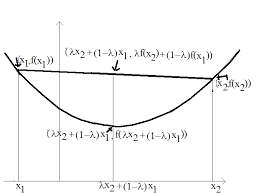
\includegraphics[width=180pt,height=180pt]{convex_function.png}
%    \caption{Primjer konveksne funkcije}
%    \label{fig:convex_function}
%\end{figure}
\begin{figure}
   \centering
\begin{tikzpicture}
\begin{axis}[width=5in,axis equal image,
    axis lines=middle,
    xmin=0,xmax=8,
    xlabel=$x$,ylabel=$y$,
    ymin=-0.25,ymax=4,
    xtick={\empty},ytick={\empty}, axis on top
]

% 
\addplot[thick,domain=0.25:7,blue,name path = A]  {-x/3 + 2.75} coordinate[pos=0.4] (m) ;
\draw[thick,blue, name path =B] (0.15,4) .. controls (1,1) and (4,0) .. (6,2) node[pos=0.95, color=black, right]  {$f(x)$} coordinate[pos=0.075] (a1)  coordinate[pos=0.95] (a2);
\path [name intersections={of=A and B, by={a,b}}];

% 
\draw[densely dashed] (0,0) -| node[pos=0.5, color=black, label=below:$a$] {}(a1);
\draw[densely dashed] (0,0) -| node[pos=0.5, color=black, label=below:$x_{1}$] {}(a);
\draw[densely dashed, name path=D] (3,0) -|node[pos=0.5, color=black, label=below:$\lambda x_{1}+ (1-\lambda)x_{2}$] {} node[pos=1, fill,circle,inner sep=1pt] {}(m);
\draw[densely dashed] (0,0) -|node[pos=0.5, color=black, label=below:$x_{2}$] {}(b);
\draw[densely dashed] (0,0) -|node[pos=0.5, color=black, label=below:$b$] {}(a2);

% 
\path [name intersections={of=B and D, by={c}}] node[fill,circle,inner sep=1pt] at (c) {}; 

% 
\node[anchor=south west, text=black] (d) at (0.75,3) {$f[\lambda x_{1}+(1-\lambda)x_{2}]$};
\node[anchor=south west, text=black] (e) at (5,2.5) {$\lambda f(x_{1})+(1-\lambda)f(x_{2})$};
\draw[-{Latex[width=4pt,length=6pt]}, densely dashed] (d) -- (c);
\draw[-{Latex[width=4pt,length=6pt]}, densely dashed] (e) -- (m);
\end{axis}
\end{tikzpicture}
   \caption{Konveksna funkcija: geometrijska interpretacija.}
   \label{fig:convex_function}
\end{figure}

\begin{definition}
   Neka su dati vektori $z^i \in \mathbb{R}^n$,  te $\lambda_i \in [0,1]$ $i=1,\ldots,m$ tako da je $\sum_{i=1}^m \lambda_i = 1.$ Vektor $x =  \sum_{i=1}^m \lambda_i z^i$ je  konveksna kombinacija vektora $z^i$.
\end{definition}

Konveksne funkcije imaju dosta poželjna svojstva sa teoretskog stanovišta i u kombinaciji sa konveksnim skupovima čine osnov u teoriji optimalnosti. 

\begin{thm}
  Neka je $f : S \mapsto \mathbb{R}$ konveksna funkcija definisana na konveksnom skupu $S \subseteq \mathbb{R}^n$. Ako funkcija $f$ u tački $x^* \in S$
 postiže lokalni minimum, onda je ta tačka i tačka globalnog minimuma.
\end{thm}
\begin{proof}  
 Neka je $x^* \in S$ tačka lokalnog minimuma funkcije $f$. Prema tome, postoji $r >0$ za što vrijedi $f(x^*) \leq f(x)$, za sve $x \in S \cap K(x^*, r)$. Odaberimo vektor $x \neq x^* \in S$ i definišimo vektor 
 $z(\lambda) = \lambda x + (1 - \lambda) x^*$ za neki $\lambda \in [0, 1]$. Kako je $S$ konveksan, slijedi da je $z \in S$.  Definišimo $\lambda_0 <  \min\{1, r ||x - x^*||^{-1}\}$, $\lambda_0 \in (0, 1]$. Tada za svaki $\lambda \in (0, \lambda_0)$ vrijedi 
 \begin{equation}
     ||z(\lambda) - x^* ||  =  || \lambda ( x - x^*) ||  = \lambda ||x - x^* || \leq \lambda_0 ||x - x^* ||  \leq r.
 \end{equation}
 Dakle, pokazano je da je $z(\lambda) \in S \cap K(x^*, r)$. Prema tome, vrijedi 
 \begin{equation}
     f(x^*) \leq f(z(\lambda)) = \lambda f(x) + (1-\lambda) f(x^*) 
 \end{equation}
 odakle slijedi 
 \begin{equation}
      \lambda f(x^*) \leq   \lambda f(x) \Rightarrow f(x^*) \leq f(x),  
 \end{equation}
 za proizvoljno odabrano $x \in S$, čime smo pokazali teoremu. 
\end{proof}
% http://home.ku.edu.tr/~mturkay/indr262/Indr262LectureNotes_2-LPModels.pdf
% (Assumptions of Linear Programming)
\\
U sljedeće dvije definicije definišimo pojmove poliedra, hiperravni i poluprostora. 

\begin{definition}
   Neka je $A \in \mathbb{R}^{m \times n}, b \in \mathbb{R}^m$. Skup $P=\{x \in \mathbb{R}^n \mid Ax \geq b\}$ se naziva poliedar u $\mathbb{R}^n$. 
\end{definition}
\begin{definition}
   Neka je $a\in \mathbb{R}^n $ i $b \in \mathbb{R}$. Skup $\{ x \in \mathbb{R}^n \mid a^T x = b \}$ se naziva hiperravan u $\mathbb{R}^n$ (sa vektorom normale $a$), dok se $\{ x \in \mathbb{R}^n \mid a^T x \geq b \}$ naziva poluprostor. 
\end{definition}
Pokažimo sada da je poliedar konveksan skup. To je veoma bitno, jer, kako znamo, uslovi  problema LP-a se mogu zapisati kao poliedar, a ako je on konveksan skup, prethodna teorema nam kaže da se onda može naći globalni minimum (maksimum), tj. optimalno rješenje zadanog problema LP-a (ako je nađen lokalni).
\begin{prop}
  ($i$) Poluprostor u $\mathbb{R}^n$ je konveksan skup.  \\
  ($ii$) Presjek konačno mnogo skupova je konačan skup. \\
  ($iii$) Poliedar u $\mathbb{R}^n$ je konveksan skup. 
\end{prop}

\begin{proof}
  ($i$) Neka je dat poluprostor $P = \{ x \in \mathbb{R}^n \mid a^T x \geq b \}$. Uzmimo $x, y \in P$, te neko $\lambda \in [0, 1]$. Treba da pokažemo da konveksna kombinacija ova dva vektora takođe pripada $P$. Iz $x \in P$, slijedi  $a^T x \geq b$. Takođe, kako je $y \in P$, to je  $a^T y \geq b$. 
  Sada jednostavno slijedi sljedeće:
  \begin{align}
      a^T (\lambda x) \geq \lambda b \\
      a^T ((1-\lambda) y) \geq (1-\lambda) b 
  \end{align}
  Sabirajući posljednje dvije nejednakosti, dobijamo 
  \begin{equation}
      a^T( \lambda x + (1 - \lambda) y ) \geq b,
  \end{equation}
  odakle slijedi da $\lambda x + (1-\lambda) y \in P$, odakle slijedi tvrdnja. 
  
  ($ii$) Neka su $S_1,\ldots, S_n$ konveksni skupovi. Ako $x,y \in \cap_{i=1}^n S_i$, onda slijedi da $x,y \in S_i$ za svaki $i=1,\ldots,n$. Zbog konveksnosti svakog od skupova,  
  $\lambda x + (1 - \lambda) y \in S_i$, za svaki $i=1,\ldots,n$. Prema tome, vrijedi $ \lambda x + (1-\lambda) y \in \cap_{i=1}^n S_i$, odakle slijedi da je $\cap_{i=1}^n S_i$ konveksan. \\
  
  ($iii$) Definišimo $S_i:= \{ (x_1,\ldots, x_n) \in \mathbb{R}^n \mid c^T x \geq b_i \}$, za  $c = (a_{i,1}, \ldots, a_{i, n}),$  $ i=1,\ldots, m$. Kako je $\cap_{i=1}^m S_i$ poliedar koji odgovara problemu LP-a, iz ($ii$) slijedi tvrdnja. 
\end{proof}

Nadalje, formalno definišimo ekstremne tačke, vrhove i bazna dopustiva rješenja koja su već ranije pomenuta u nestriktnom obliku. 

\begin{definition}
   Neka je $P$ poliedar u $\mathbb{R}^n$.  Vektor $x \in P$ se naziva ekstremna tačka poliedra $P$
   ako ne postoje vektori $y, z \in P$, $y \neq x, z \neq x$ i skalar $\lambda \in [0, 1]$ takvi da je  $x = \lambda y + (1-\lambda)z$.
\end{definition}
Geometrijska interpretacija ekstremnih tačkača poliedra:  One tačke koje se ne mogu napisati kao netrivijalna konveksna kombinacija tačaka iz poliedra čine skup ekstremnih tačaka. 
 
\begin{definition}
   Neka je dat poliedar $P$ u $\mathbb{R}^n$. Tačku $x \in P$ nazivamo vrh (poliedra) ako postoji $c \in \mathbb{R}^n$ tako da za sve y $\in P, y \neq x$, vrijedi $c^T x < c^T y$. 
\end{definition}
Geometrijski bi to značilo da je vrh poliedra $P$ ona tačka poliedra  kroz koju možemo provući hiperravan sa svojstvom da se sve tačke iz $P$ (izuzev vrha) nalaze s iste strane te poluravni.

\begin{definition}\label{dfn:lp_aktivan}
   Neka je poliedar $P$ zadan na sljedeći način
   \begin{itemize}
       \item $a_i^T x \geq b_i, i \in M_1$
       \item $a_i^T x = b_i, i \in M_2 $
       \item $a_i^T x \leq b_i, i \in M_3 $. 
   \end{itemize}
   Ako za neko $x^* \in P$ i neki $i_0 \in M_1 \cup M_1 \cup M_2$ vrijedi 
   $a_{i_0}^T x^* = b_{i_0}$, onda je uslov $i_0$ aktivan u $x^*$. 
\end{definition}

\begin{definition}
      Neka je zadan poliedar iz Definicije~\ref{dfn:lp_aktivan}. Neka je 
      $I = \{ i \in M_1 \cup M_2 \cup M_3 \mid a_i^T x^* = b_i \}$  skup indeksa aktivnih u $x^*\in \mathbb{R}^n$.  Ako je skup $\{ a_i \mid i \in I \}$ linearno nezavisan onda se $x^*$ bazno rješenje. Bazno rješenje $x^*$ se naziva bazno dopustivo rješenje ako zadovoljava sve uslove linearnog programiranja. 
\end{definition}

\begin{thm}
   Neka je $P$ poliedar i neka je $x^* \in P$. Sljedeće tri tvrdnje su ekvivalentne:
   \begin{enumerate}
       \item $x^*$ je vrh poliedra;
       \item $x^*$ je ekstremna tačka poliedra;
       \item $x^*$ je bazno dopustivo rješenje (BDR).
   \end{enumerate}
\end{thm}

\begin{proof}
      Pokažimo da vrijedi $1 \Rightarrow 2, 2 \Rightarrow 3$, pa onda $3 \Rightarrow 1$, čime pokazujemo ekvivalenciju sve tri tvrdnje. \\
      $1 \Rightarrow 2$. Neka je $x^*$ vrh poliedra. Iz definicije slijedi da 
      postoji $c\in \mathbb{R}^n$ tako da $c^Tx^* < c^T x$, za sve $x \in P, x \neq x^*$. Pretpostavimo da $x^*$ nije ekstremna tačka poliedra $P$. To bi značilo da postoje $y,z \in P$ koji su ražličiti od $x^*$ koji se može dobiti kao (netrivijalna) konveksna kombinacija $y$ i $z$, tj. $x^* = \lambda y + (1 - \lambda) z $, za $\lambda \in [0,1 ]$. Na osnovu pretpostavke je $c^T x^* < c^T y$. Sada je 
      \begin{align}
          &c^T x^* = c^T ( \lambda y + (1 - \lambda) z )  = c^T( \lambda y) + c^T((1- \lambda) z) < \nonumber \\
          &< \lambda c^T x^* + ( 1 - \lambda) c^T x^* = c^T x^*.
      \end{align}
      što je nemoguće, odakle slijedi tvdrnja. \\
      $2 \Rightarrow 3$.
       Ovu implikaciju ćemo dokazati kontrapozicijom. Pretpostavimo da $x^*$ nije BDR i pokažimo da iz toga slijedi da ona nije ni ekstremna tačka.
       Zapišimo poliedar $P$ sa 
       \begin{align}
            & a_i^T x \geq b_i, i \in M_1 \\
            & a_i^T x  = b_i, i \in M_2.
       \end{align}
       Ako $x^*$ nije BDR, to znači da je broj uslova koji su aktivni u $x^*$ manji od $n$. 
       Ako sa $I \subseteq M_1 \cup M_2$ označimo skup aktivnih indeksa, onda 
       je $\{ a_i \mid i \in I \} \subseteq \mathbb{R}^n$ pravi potprostor od $\mathbb{R}^n$.  Prema tome, postoji vektor $d \in \mathbb{R}^n \setminus \{0\}$ za koji vrijedi $a_i^T d = 0$, za sve $i \in I$. Definišimo vektore 
       $$ y = x^* + \epsilon d, z = x^* - \epsilon d, $$
       za neko $\epsilon > 0$, pa pokažimo da $y, z \in P$.
       
       Ako je $i \in I$, onda je $$a_i^T y = a_i^T (x^* + \epsilon d) = a_i^T x^* + \epsilon a_i^T d = a_i^T x^* = b_i. $$
       Pokažimo još da za $i \not \in I$ vrijedi $a_i^T x^* > b_i$, odakle bi slijedilo da $y \in P$. Dakle, $a_i^T y = a_i^T (x^* + \epsilon d) = a_i^T x^* + \epsilon a_i^T d $. Ako je $a_i^T d \geq 0$, slijedi da je 
       $a_i^T x^* > b_i$, odakle slijedi da je $y \in  P$. Ako je $a_i^T d < 0$, onda odaberimo takve $\epsilon$ za koje će vrijediti $a_i^T x^* + \epsilon a_i^T d > b_i$. Interval   vrijednosti za $\epsilon$ dobijemo iz sljedećeg računa:
       $$ a_i^T x^* + \epsilon a_i^T d > b_i \Rightarrow \epsilon < \frac{b_i - a_i^T x^*}{a_i^T d}  $$
       Za svaki $\epsilon \in (0,  \frac{b_i - a_i^T x^*}{a_i^T d} )$ vrijedi $a_i^T y > b_i$, odakle slijedi $y \in P$. Slično pokažemo i da vrijedi $z \in P$. 
       Prema tome lako je vidjeti da vrijedi $x^* = \frac{1}{2}y +\frac{1}{2} z$, dakle $x^*$ se dobija kao netrivijalna konveksna kombinacija, što je u suprotnosti sa definicijom ekstremne tačke. \\
       $3 \Rightarrow 1$. Neka je $x^*$ BDR. Treba da pokažemo da je ona takođe vrh poliedra $P$. Iz pretpostavke, za BDR, označimo sa $I$ skup aktivnih indeksa u $x^*$ i definišimo $c = \sum_{i \in I} a_i$.  Tada imamo 
       $ c^T x^* = \sum_{i \in I } a_i^T x^* = \sum_{i \in I} b_i$. Za proizvoljno $x \in P$ dobijamo
       \begin{equation}\label{eq:3_impl_1}
          c^T x = \sum_{i \in I} a_i^T x \geq c^T x^*  
       \end{equation}
     Iz toga vidimo da je $x^*$ rješenje LP problema minimizacije. Jednakost u (\ref{eq:3_impl_1}) vrijedi ako i samo ako je $a_i^T x = b_i$ za sve $i \in I$. Kako je $x^*$ BDR, broj linearno nezavisnih vektora $a_i, i \in I$ koji su  aktivni u $x^*$ je jednak $n$, pa sistem $a_i^T x = b_i, i \in I$ ima jedinstveno rješenje koje je upravo $x^*$. Prema tome, pokazano je da postoji vektor $c \in \mathbb{R}^n$ za koji vrijedi $c^T x > c^T x^*$ za sve $x \neq x^*$, $x \in P$, odake na osnovu definicije vrha poliedra, slijedi tvrdnja. 
\end{proof}

U nastavku ćemo vidjeti koji sve uslovi treba da vrijede za postojanje BDR-a
i ekstremne tačke poliedra. Takođe ćemo dati postupak za konstrukciju BDR-a te ćemo definisati degenerativno rješenje.

\begin{thm}
   Neka je $P = \{ x \in \mathbb{R}^n \mid A x = b, x \geq 0\}, A \in \mathbb{R}^{m \times n}, b \in \mathbb{R}^m$ i $rang(A)= m, m < n$.
   Vektor $x$ je bazno rješenje  akko je $A x = b$ i ako postoje indeksi $p_1,p_2,\ldots, p_m$ tako da vrijedi:
   \begin{enumerate}
       \item kolone $A_{p_1},\ldots, A_{p_m}$ su linearne nezavisne
       \item ako $i \in \{p_1,\ldots, p_m\}$, onda $x_i = 0$.
   \end{enumerate}
   
\end{thm}
Postupak konstrukcije baznog rješenja je dat sljedećim koracima:
\begin{enumerate}
    \item Odabrati $m$ linearno nezavisnih kolona $A_{p_1}, \ldots, A_{p_m}$ matrice $A$.
    \item Postaviti $x_i = 0$, za sve $i \in \{p_1,\ldots, p_m \}$.
    \item Riješiti sistem $B x_B = b$, za $x_B = [x_{p_1}, \ldots, x_{p_m}]$ i $B= [A_{p_1}, \ldots, A_{p_m}]$
    \item Vektor $x = (x_1,\ldots, x_n)$ za koje je $x_j = 0$ za $j  \not \in \{p_1,\ldots, p_m \}$ ili $x_{p_i} = (x_B)_i$ za $j = p_i$ je bazno rješenje. 
\end{enumerate}
Varijable $x_{p_1},\ldots, x_{p_m}$ nazivamo bazne varijable, a vektore  $A_{p_1}, \ldots, A_{p_m}$ bazni vektori, indekse $p_1,\ldots, p_m$ bazni indeksi, dok matricu $B$ matrica baze. 


Definišimo sada pojam \emph{degenerativnog} rješenje i degenerativnog baznog rješenja. Pokazaćemo kako se na primjeru pronalazi bazno rješenje te kako izgleda degenerativno bazno rješenje.

\begin{definition}
      Neka je dat poliedar $P = \{ x \in \mathbb{R}^n \mid a_i^T x \geq b_i, i=1,\ldots,m \}$. Za bazno rješenje $x^*\in \mathbb{R}^n$ kažemo da je degenerativno ako je više od $n$ uslova (ograničenja) aktivno u $x^*$. 
      
\end{definition}

\begin{definition}
      Neka je $P = \{ x \in \mathbb{R}^n \mid A x = b, x \geq 0\}, A \in \mathbb{R}^{m \times n}, b \in \mathbb{R}^m$ poliedar u standardnom obliku i neka je $x$ bazno rješenje. Vektor $x$ nazivamo degenerativno bazno rješenje ako više od $n-m$ komponenti u vektoru $x$ je jednako 0.
\end{definition}
\emph{Primjer.} Zadajmo poliedar $P= \{ (x_1,x_2,x_3)^T \mid x_1 - x_2 = 0, x_1 + x_2 + 2 x_3 = 2, x_1,x_2,x_3 \geq 0 \}$.  Promaći bazna dopustiva rješenja i odrediti jesu li ona degenerativna. \\

\emph{Rješenje.} Lako je vidjeti da je  
$A=\left (\begin{array}{ccc}
   1  & -1 & 0  \\
   1  &  1 & 2 \\
\end{array} \right )$ te $b = [0\ 2]^T$. Prateći postupak konstrukcije baznog rješenja, pronađimo dve linearno nezavisne kolone matrice $A$, recimo prve dvije, odakle je matica $B=\left (\begin{array}{cc}
   1  & -1    \\
   1  &  1   \\
\end{array} \right ) .$ Riješimo sistem jednačina (stavka 3), odakle je rješenje $x_B = [1\ 1]^T$, a krajnje rješenje je $x^* = [1\ 1\ 0]^T$. Kako je 
$x^*$ aktivan u sva tri uslova $x_1 - x_2 = 0, x_1 + x_2 + 2 x_3 = 2$ i $x_3 = 0$, rješenje je nedegenerativno bazno dopustivo rješenje.  Takođe, možemo odabrati drugu i treću kolonu matrice za bazne kolone (kao i prvu i treću), odakle bi dobili rješenje $x^* = [0\ 0\ 1]^T$, aktivno u četiri uslova, odakle smo dobili degenerativno bazno dopustivo rješenje. 


U nastavku govorimo o egzistenciji optimalnog rješenja problema LP-a.

\begin{definition}
      Poliedar $P$ sadrži pravac akko postoji $x \in P$ i $d \in \mathbb{R}^n \setminus \{0\}$ tako da je $x + \lambda d \in P$, za sve $\lambda \in \mathbb{R}$. 
\end{definition}

Sljedeću teoremu navodio bez dokaza.

\begin{thm}
   Neka je dat poliedar $P=\{ x \in \mathbb{R}^n  \mid a_i^T x \geq b_i, i=1,\ldots,m\} $. Tada su sljedeće tri tvrdnje ekvivalentne:
   \begin{itemize}
       \item  Poliedar $P$ ima barem jednu ekstremnu tačku.
       \item Poliedar $P$ ne sadrži pravac.
       \item Postoji $n$ linearno nezavisnih vektora  među kolonama matrice $A$, tj. među $a_i, i=1,\ldots,m$.
   \end{itemize}
\end{thm}

\begin{thm}
   Neka je zadan problem LP-a sa funkcijom cilja $c^Tx$ koju je potrebno minimizovati na poliedru $P$. Pretpostavimo da za poliedar $P$ postoji barem jedna ekstremna tačka i da za dati problem postoji optimalno rješenje. Tada postoji i optimalno rješenje koje je ekstremna tačka poliedra $P$.
\end{thm}

\begin{proof}
         Sa $O^* \not = \emptyset$ označimo skup svih optimalnih rješenja LP problema nad poliedrom $P= \{ x \in \mathbb{R}^n \mid A x \geq b \}$ te neka je $c^T x^* = v$, za sve $x^* \in O^*$. Vidimo da je 
         $O^* = \{ x \in \mathbb{R}^n \mid A x \geq b_i, c^T x = v  \}$ je takođe poliedar, $O^* \subset P$. Prethodna teorema nam kaže da $P$ ne sadrži pravac. Iz toga slijedi da ni $O^*$ nema pravac, odakle slijedi da $O^*$ ima barem jednu ekstremnu tačku, označimo je sa $q^*$. Pokažimo da je to i ekstremna tačka od $P$.  Ako bi pretpostavili da $q^*$ nije ekstremna tačka, po definiciji slijedi da postoje $y, z \in P$ tako da $q^* = \lambda y + ( 1 - \lambda ) z $, $y \neq q^*, z \neq q^*, \lambda \in [0, 1]$. Kako je $q^* \in O^*$, imamo 
         $$ v = c^T q^* = c^T (  \lambda y + ( 1 - \lambda ) z ) = \lambda 
        \underbrace{ c^T y}_{ \geq v} + ( 1 - \lambda ) \underbrace{c^T z}_{\geq v} \geq \lambda v + (1 - \lambda) v = v,$$
        odakle imamo $c^T y = v$ i $c^T z = v$, dakle $y, z \in O^*$. Prema tome, $q^*$ nije ekstremna tačka od $O^*$. Prema tome, imam kontradikciju, odakle slijedi da $q^*$  ekstremna tačka od  $P$.
\end{proof}
 
 Sljedeća teorema nam daje osnov za konstrukciju simpleks metoda koji je najpoznatija metoda za rješavanje problema LP.
 
 \begin{thm}
   Riješimo problem minimizacije LP-a na poliedru $P$ koji ima barem jednu ekstremnu tačku. Tada vrijedi jedna od sljedeće dvije tvrdnje:
   \begin{enumerate}
       \item Funkcija cilja ima vrijednost $- \infty$ (neograničen).
       \item Postoji ekstremna tačka koja je optimum problema. 
   \end{enumerate}
 \end{thm}
To nam daje opravdanost ideje simpleks metode koja posjećuje vrhove poliedra 
da bi našao optimalno rješenje problema LP-a. Metodu opisujemo u narednoj glavi.

\newpage 
\section{Simpleks Metod}

Simpleks metoda je najpoznatija metoda za rješavanje problema linearnog programiranja. Simpleks metoda traži rješenje LP-a posjećujući vrhove poliedra krećući se po njegovim granicama  uvijek u smijeru smanjenja vrijednosti
funkcije cilja (ako je dat zadatak minimizacije). Razvio ju je George Dantzig 1947. godine i spada među najznačajnije algoritme XX vijeka.

Neka je dat problem LP-a u obliku:

\begin{align}
    &c^Tx \rightarrow \min \nonumber \\ 
    & A x = b \nonumber \\
     & x \geq 0, \label{eq:lp_equality_constraint}
\end{align}
gdje je $A \in \mathbb{R}^{m \times n}, b \in \mathbb{R}^m, c \in \mathbb{R}^n, x\in \mathbb{R}^n$ uz pretpostavku da je poliedar $P=\{ x \in \mathbb{R}^n \mid A x = b , x \geq 0 \}$ datog problema LP-a dopustiv.  U ovom poglavlju, osim ako drugačije nije naznačeno, strogo ćemo poštovati ovu notaciju. 

\begin{definition}
      Za matricu A kažemo da je regularna akko postoji matrica B td. AB = BA = I. 
\end{definition}

\begin{definition}
      Za pravac $d\in \mathbb{R}^n$ kažemo da je dopustiv u tački $x \in P$ akko postoji $\lambda > 0$ tako da $x + \lambda d \in P$.
\end{definition}

\subsection{Konstrukcija simpleks metode}

 Neka je $x = [x_1,\ldots, x_n]^T$ bazno dopustivo rješenje poliedra $P$, gdje je $B$ matrica baze, $x_B$ bazni dio vektora $x$, a gdje su na mjesto nebaznih indeksa $N$ postavljene 0.  Sobzirom da je $x$ BDR, a kako je ideja metode ``šetanje'' po ivici poliedra  do drugog dok ne nađemo optimalno rješenje, krenimo pravcem $d$ u  tački $x$ (koju  treba da konstruišemo) pri čemu moramo paziti na to da
\begin{itemize}
    \item je zadovoljen \emph{uslov optimalnosti}, tj. $c^T (x + \lambda d) \leq c^T x$, što znači da idemo u pravcu smanjenja vrijednosti funkcije cilja;
    \item je zadovoljen \emph{uslov dopustivosti}, tj. $ (x + \lambda d) \in P$. Dakle, krećemo se samo tačkama dopustivog regiona. 
\end{itemize}
Birajmo nebaznu koordinatu u $x$, neka je to $x_j, j \in N$. Definišemo $d_j =1$, $d_i = 0$, za sve $i \in N  \setminus \{j\}$. Time smo definisali nebazni
dio vektora $d$. Bazni dio vektora $d$, kojeg označavamo sa $d_B$, izvešćemo iz uslova dopustivosti: $Ax + \lambda Ad = b$, odakle je $Ad = 0$. Tada je 
$$ Ad = \sum_{i=1}^n A_i d_i = \sum_{i=1}^m A_{p_i} d_i + A_j = B d_B + A_j = 0$$
odakle je $d_B = -  B^{-1} \cdot A_j $.  Za ovako dabran $d$ imamo zadovoljen uslov dopustivosti $A( x + \lambda d )  =b$, još provjerimo uslov nenegativnosti koji vrijedi u LP-u, tj. $x + \lambda d \geq 0$:
\begin{itemize}
    \item ako je $x$ nedegenerativno, onda je tačno $n-m$ komponenti jednako 0,       pa je za nebazni dio komponenti $x_i + \lambda d_i = 0$, za $i \in N \setminus \{j\}$, dok je $x_j + \lambda d_j = 0$, pa imamo ispunjen uslov nenegativnosti. Za bazne komponente imamo $x_{p_i} \cdot d_{p_i} > 0 $ ako je $d_{p_i}>0$. U protivnom, možemo odabrati  malu vrijednosti $\lambda>0$ (pogledati definiciju $x +\lambda d$) tako da $x_{p_i} \cdot d_{p_i} >0$, pa imam zadovoljen uslov nenegativnosti.
    \item ako je $x$ degenerativno bazno dopustivo rješenje, slijedi da više od $n-m$ kompomenti od $x$ je jednako 0. Za nebazni slučaj kao i u prvom slučaju pokazujemo uslov nenegativnosti. Za bazne kompomenete $x +\lambda d$,  postoji bazni indeks $i$ za koji je $x_{p_i} = 0$, pa   je $d_{p_i}< 0$, što povlači da ne možemo naći $\lambda>0$ tako da $x_{p_i} + \lambda d_{p_i} >0$  što stvara problem (dopustivost narušena), ali pojava ovog slučaja se na sreću može zaobići (pokazaćemo to u nastavku ove sekcije). 
\end{itemize}
 Ostaje kako odabrati nebaznu varijablu $x_j$. U pomoć pozivamo uslov optimalnosti $c^T ( x + \lambda d ) > c^T x $, odakle slijedi $c^T d < 0$.  Kako je $$c^T d = c_B^T d_B + c_j = c^T ( - B^{-1} A_j ) + c_j < 0.$$
 Prema tome, odaberimo $j$ pri čemu je zadovoljeno $ \overline{c_j} = c_j - c_B^T B^{-1}A_j < 0$. Vektor $\overline{c_j}=[\overline{c_1}, \ldots, \overline{c_n}]^T$ se naziva vektor doprinosa, dok vrijednost $\overline{c_j}$ \emph{doprinos nebazne varijable} $x_j$. 
 
Iz sljedeće teoreme dobijamo uslove optimalnosti rješenja.

\begin{thm}
  Neka je x bazno dopustivo rješenje i neka je $B$ bazna matrica a $\overline{c}$ vektor doprinosa. Vrijedi 
  \begin{itemize}
      \item Ako je $\overline{c} >0$, onda je $x$ optimalno rješenje.
      \item Ako je x optimalno nedegenerativno rješenje, onda je $\overline{c} \geq 0$.
  \end{itemize}
\end{thm}

Ostalo nam je još odrediti dužinu koraka pravca $d$, tj. vrijednost $\lambda>0$. Ideja je da se krene nekim smjerom dok god se ne dođe do drugog vrha, tj. $\max \{ \lambda \in \mathbb{R} \mid x + \lambda d \geq 0 \}$. 
\begin{itemize}
    \item Ako $d >0$, onda je $  x + \lambda d \geq 0$, za sve $\lambda > 0$, pa je $\lambda^* = \infty$, tj. ciljna funkcija je neograničena.
    \item Ako postoji $i$, td. $d_i < 0$, onda odaberimo dovoljno malo $\lambda>0$ tako da $x_i + \lambda d_i \geq 0$, odakle slijedi $\lambda \leq -\frac{x_i}{d_i}$. Prema tome 
    $$ \lambda^* = \min_{ \{i\in [m] \mid d_{p_i} < 0  \}} - \frac{x_{p_i}}{d_{p_i}} $$
\end{itemize}
Za indeks $l$ za koji se postiže ovaj minimum, vrijedi $x_{p_l} + \lambda^* d_{p_l}=0$.
Da je ovo upravo bazno dopustivo rješenje problema, govori nam sljedeća teorema. 
\begin{thm}
    Kolone $A_{p_i}, i\not = l$, $i=1,\ldots,m$ i $A_{j}$ su linearno nezavisni, pa je matrica 
    $[A_{p_1},\ldots, A_{p_{l-1}}, A_j, A_{p_{l+1}}, \ldots, A_{p_m}]$
    regularna. Vektor $x + \lambda^* d$ predstavlja bazno dopustivo rješenje. 
\end{thm}

Navedimo sada osnovne korake jedne iteracije simpleks metoda:
\begin{enumerate}
    \item Inicijalizacija: za bazne indekse $p_1,\ldots,p_m \in [n]$, riješiti sistem i dobiti bazno dopustivo rješenje $x$. 
    \item Izračunati doprinos za sve $\overline{c_j} = c_j - c_B^T B^{-1}A_j $
          $j \in N$. Ako za sve $j$, $\overline{c_j} \geq 0$, optimum je nađen, algoritam staje sa radom. Inače, odabrati neki $j$, td. $\overline{c_j}<0$.
    \item Izračunati $d = -B^{-1}A_j = -u$. Ako je svaki $d_i \geq  0$, funkcija cilja je $f = - \infty$, te algoritam staje. 
    \item Ako je za neki $i$, $d_i < 0$, onda računamo 
             $$ \lambda^* = \min_{ \{i\in [m] \mid d_{p_i} < 0  \}} - \frac{x_{p_i}}{d_{p_i}} =  \min_{ \{i\in [m] \mid u_{p_i} < 0  \}} \frac{x_{p_i}}{u_{p_i}} $$
    \item Neka je $\lambda^* = \frac{x_{p_i}}{u_{p_i}}$. Nova baza se formira tako da mjesto kolone $A_{p_l}$ stavimo kolonu $A_j$. Novo bazno rješenje 
    $y = x + \lambda^*d $ je dato: $y_j = \lambda$, $y_{p_i} = x_{p_i} + \lambda^* d_{p_i}$, za $i$ koji je bazni indeks, te $y_i = 0$, za $i \in N \setminus \{j\}$. 
\end{enumerate}

\subsection{Tabelarni prikaz Simpleks Metode}

U osnovi, simpleks algoritam se sastoji od stalne izmjene jedne kolone baznih vektora u $B$ sa najboljim nebaznim vektorom i tako iterativno u cilju smanjivanja trenutne vrijednosti cilje funkcije, dok god je to moguće. 
U praktičnom računanju, baratanje sa tabelarnim prikazom koraka simpleks metoda je u mnogome lakše (kompaktnije) nego koristiti standardan oblik LP-a. 
Simpleks tabela ima oblik kao u Tabeli~\ref{tab:simplex_tabelau}. 

\begin{table}[!ht]
    \centering
    \begin{tabular}{c c c | c} \\ \hline
            $\mid$          &       $\mid$ &  $\mid$             &    $x_{p_1} = \overline{b_1}$         \\
          $B^{-1}A_1$       &    $\cdots$    &  $B^{-1}A_n$      &    $\cdots$          \\
            $\mid$          &       $\mid$ &  $\mid$             &   $ x_{p_m} = \overline{b_m}$         \\ \hline
          $\overline{c_1}$  &    $\cdots$    & $\overline{c_n}$  &  $-c^T_B x_B$         \\ \hline
    \end{tabular}
    \caption{Simpleks tabela}
    \label{tab:simplex_tabelau}
\end{table}

Na osnovu ovakve tabele, te koraka simpleks metode opisanih u prethodnoj sekciji, pratimo sljedeće korake u tabelarnom rješavanju:
\begin{itemize}
    \item Konstruisati inicijalnu simpleks tabelu sa početnom bazom $B$ i odgovarajućim baznim dopustivim rješenjem $x$.
    \item Pogledati koeficijente doprinosa $\overline{c_j}$. Ako su svi $\overline{c_j} \geq 0$, rješenje se ne može dalje popraviti, pa smo našli optimalno rješenje, inače odabrati neki $j$ sa $\overline{c_j}<0$.
    \item Pogledati vektor $u = B^{-1}A_j$. Ako su sve koordinate od $u$ negativne, rješenje LP-a je $-\infty$, algoritam se prekida.
    \item Za svaki $u_i > 0$, računati $x_{p_i}/u_i$, i neka je ovaj omjer najmanji za indeks $l$. Kolona $A_{j}$ ulazi u bazu, dok kolona $A_{p_l}$ izlazi iz baze. 
    \item Svakom redu table dodati $l$--ti red (pivot red) kojeg množimo odgovarajućim
         skalarom kako bi pivot element postao 1, a svi ostali elementi u pivot koloni 0.
\end{itemize}

U ovom postupku  može se desiti situacija da postoji dva ili više redova koji su kandidati za ulazak u bazu. Ako se odabere nepovoljan kandidat, postupak može da proizvede degenerativno BDR ili čak da dođe do ciklusa. 
Da bi se to spriječilo, Robert Bland (1977. godine) je uveo pravilo za pivotiranje danas poznato pod
nazivom \emph{Blandovo pravilo} koje:
\begin{enumerate}
	\item   Među svim nebaznim varijablama koje su pogodne za ulazak u bazu odaberemo onu najmanjeg indeksa. 
    \item Među svim baznim varijablama koje su pogodne za izbacivanje iz baze odaberemo onu s najmanjim indeksom.
\end{enumerate}
Može se pokazati da poštujući ovakva pravila, osigurava se da simpleks metoda  završava u konačno mnogo koraka.
Obratimo pažnju da se problem minimiziacije vrlo lako prevodi u problem maksimizacije sljedećom transformacijom
$$ \min_{ x \in P} f(x) = - \max_{x \in P}(-f(x)).$$ 
Prema tome, ako imamo problem LP-a gdje treba da maksimizujemo vrijednost funkcije cilja, pa onda primijenimo simpleks metod, koraci metoda ostaju isti, uz malu izmijenu u koraku 2, gdje se mijenja znak nejednakosti (radi toga što se mijenja znak koeficijenata u funckciji cilja). Dakle, za popravak rješenja bi u tom slučaju gledaji one doprinose za koje je $\overline{c_j} > 0$.

\subsection{Primjer rješavanja problema LP-a pomoću Simpleks Metoda}
Kako je standardni politop LP-a dat sa svim onim $x \in \mathbb{R}^n$ tako da $Ax \leq (\geq) b$, transformišimo problem LP-a
 
  \begin{align}
    & c^T x \rightarrow \max \\
    & Ax \leq b \\
    & x \geq 0,\\
\end{align}
 
na oblik pogodan simpleks metodi $(A {x} = b)$ dodavanjem ``labavih'' varijabli $s$ na sljedeći način:
 
\begin{align}
    & c^T x \rightarrow \max \\
    & Ax + s =  b \\
    & x \geq 0, s \geq 0. \\
\end{align}
što u matričnom obliku odgovara 

\begin{align}
    & c^T x \rightarrow \max \\
    & (A | I) \cdot \left (\begin{array}{c}
         x  \\
         s 
    \end{array} \right ) =  b \\
    & (x, s) \geq 0. \\
\end{align} 

U primjeru kojeg rješavamo, neka je dat problem LP-a:
\begin{align*}
    & x_1 + x_2 \rightarrow \max \nonumber \\
    & x_1 + 3 x_2 \leq 9 \nonumber \\
    & 2x_1 + x_2 \leq 8  \nonumber \\
    & x_1, x_2 \geq 0. \nonumber \\
\end{align*}
 
 Pretvarajući ga dodavajući labave varijable $s = (x_3, x_4)>0$, dobijamo 

\begin{align*}
    & x_1    & + 3x_2  &+ x_3& &= 9 \\
    & 2 x_1 &   + x_2  & + x_4& &= 8 \\
    & x_1   &   + x_2  &\  & &= f - 0 \\
\end{align*}
 Ovaj problem odgovara simpleks tabeli \\
 \begin{table}[]
     \centering
     \begin{tabular}{c c c c | c}
     	 $x_1$ & $x_2$ &  $x_3$ & $x_4$ & \\ \hline
         1 &  3  & 1 & 0 & 9 \\
         2 &  1  & 0 & 1 & 8 \\ \hline
         1 &  1  & 0  & 0 & 0 \\ \hline
     \end{tabular}
     \caption{Inicijalna simpleks tabela.}
     \label{tab:simpleks_tabela1}
 \end{table} \\
 Na početku uzmemo za bazu vektore $x_3$ i $x_4$. Prema tome, bazno dopustivo rješenje je $x = (0, 0, 9, 8)$, za koji je $f =0$. Sada ažiriramo simpleks tabelu izvodeći pivotiranje. Izaberimo indeks $j$ td. $\overline{c_j}>0$. Neka je $j=1$, i on odgovara varijabli $x_1$ čiju vrijednost želimo da povećamo u funckiji cilja. Izaberimo pivot vrstu. Gledamo odnos $\overline{b_i}/\overline{a}_{1,j}$, za sve $\overline{a}_{1,j} > 0$,  $B^{-1} A_1 = \overline{a}_{1,j}$
 i tražimo onaj indeks koji minimizuje datu vrijednost. Imamo dvije mogućnosti, $9/1$ i $8/2$, pa je $i = 2$ traženi indeks. Dakle, pivot je element $\overline{a}_{1,2}=2$. Sada radimo standardne operacije pivotiranja oko ovog elementa,  tako da sve elemente u koloni 1 simpleks matrice učinimo nulama, dok je element u drugoj vrsti 1 (Gausove eliminacije u rješavanju sitema jednačina). Primjera radi, vrsti 1 se dodaje druga vrsta pomnožena sa -$\frac{1}{2}$. Druga vrsta se dijeli sa $\frac{1}{2}$. Dok trećoj vrsti se dodaje takođe druga vrsta pomnožena sa -$\frac{1}{2}$. 
 Primjenjujući ove transformacije, dobijamo simpleks tabelu:
 
  \begin{table}[!ht]
     \centering
     \begin{tabular}{c c c c | c}
         0 &  $\frac{5}{2}$  & 1 & -$\frac{1}{2} $& 5 \\
         1 &  $\frac{1}{2}$ & 0 & $\frac{1}{2}$ & 4 \\ \hline
         0 &  $\frac{1}{2}$ & 0 & -$\frac{1}{2}$ & -4 \\ \hline
     \end{tabular}
     \caption{Simpleks tabela: nakon transformacija.}
     \label{tab:simpleks_tabela2}
 \end{table}
Bazne varijable prepoznjemo jer odgovarajući vektori (kolone) zajedno čine jediničnu matricu. Prema tome, 
 nebazne varijable su $x_2$ i $x_4$, koje dobijaju vrijednost 0, dok ostale lako izračunavamo, tj. $ x = (4, 0, 5, 0)$. Ponavljamo opet korake, nalazimo pivota, tj. poziciju  $(i,j)$. Lako je vidjeti da kolona 2 jedina odgovara nalasku odgovarajućeg pivot elementa. Dalje, za pogodnu vrstu $i$, imamo da je $5 / (5/2) < 4 / (1/2)$, prema tome $i =1$. Dakle pivot je 
 $\overline{a}_{1,2} = \frac{5}{2}$. Radimo opet gausove eliminacije oko prve vrste, pa se dobija simpleks tabela:
 
   \begin{table}[!ht]
     \centering
     \begin{tabular}{c c c c | c}
         0 &  $1$  & $\frac{2}{5}$             &  -$\frac{1}{5} $ & 2 \\
         1 &  0    &      -$\frac{1}{5}$    & $\frac{3}{5}$    & 3 \\ \hline
         0 &  0    &   -$\frac{1}{5}$       &   -$\frac{2}{5}$   & -5 \\ \hline
     \end{tabular}
     \caption{Simpleks tabela: korak 2.}
     \label{tab:simpleks_tabela2}
 \end{table}
 Kako su sve varijable doprinosa manje (ili jednakom) 0, zaključujemo da smo našli optimum koji je jednak $x = (3, 2, 0, 0)$, a optimalna vrijednost je $f = 5$.
 
 \begin{figure}[!ht]
     \centering
     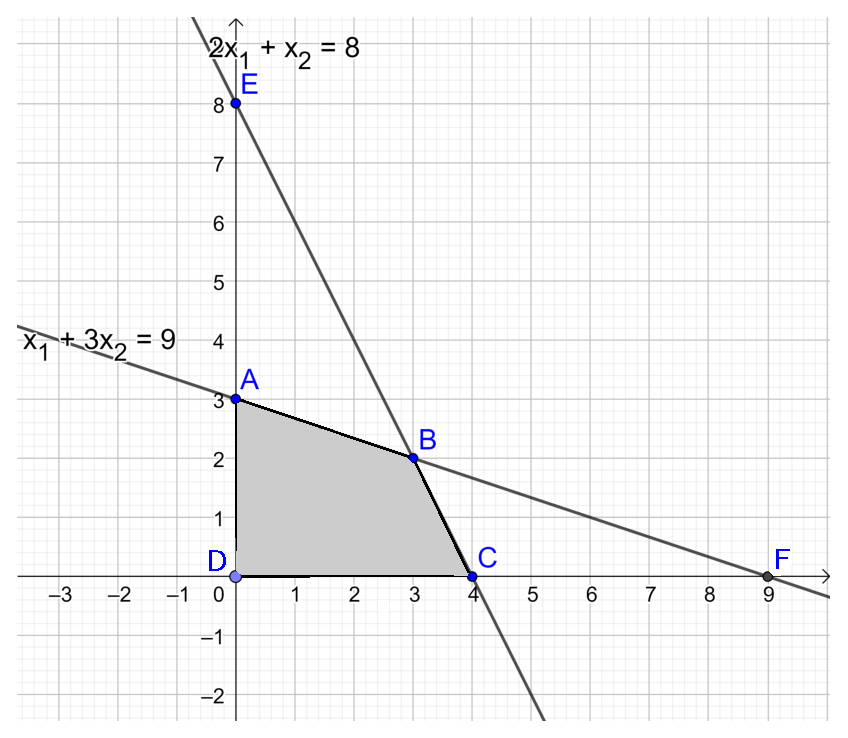
\includegraphics[width=170pt, height=170pt]{simpleks-region-2.eps}
     \caption{Region (bazna rješenja označena).}
     \label{fig:simplex_region} 
 \end{figure}
 
 \emph{Komentari na zadatak}. Na Slici~\ref{fig:simplex_region}, tačke $A, B, C$, i $D$ su bazna dopustva rješenja (BDR). Tačke $E$ i $F$ su takođe bazna rješenja, ali nisu dopustiva. Simpleks algoritam prvo kreće od tačke $A$, pa prema tački $D$, te završava u tački $C$ (optimum).
 
 \emph{Komentari na simpleks tabelu}:
 \begin{itemize}
     \item Jedinična matrica $m \times m$   ugrađena u gornju lijevu podmatricu simpleks tabele (blok sa elementima $\overline{a}_{i,j}$) sadrži kolone koji čine vektore baznih varijabli.
     \item U ovim kolonama u posljednjoj vrsti (ciljna vrsta) se nalaze nule.
 \end{itemize}
 Prema tome, vektori $x_i$, koji su bazni vektori (kolone baze $B$), su napisani preko nebaznih vektora $x_i \in N$. Kako se stavljaju $x_i  = 0$, za sve $i \in N$, onda je trivijano dobiti vrijednosti baznih vektora $x_i$, tj. kolona baze $B$. 
 
 \subsection{Dvofazni simpleks algoritam}
 Postoje dva pitanja koja se nameću u primjeni simpleks algoritma:
 \begin{itemize}
     \item Da li se uvijek može naći bazno dopustivo rješenje za početno rješenje 
     simpleks algoritma?
     \item Da li se simpleks algoritam uvijek prekida, tj. da li uvijek ili nalazi optimalno rješenje ili se zaključi da je funkcija cilja neograničena?
 \end{itemize}
 
 Odgovor na prvo pitanje je ako postoji jedinična podmatrica $I_m$ u gornjoj lijevoj blok matrici simpleks tabele,  onda je to jednostavno odrediti (kako smo to i vidjeli u prethodnoj sekciji). 
 Linearnom programu koji sadrži ograničenja $Ax \leq b, x\geq 0$ se dodaju labave varijable da bi uslovi nejednakosti u ograničenjima postali potrebne jednakosti. Na taj način se i formira ova jedinična matrica. Međutim, šta ako uslovi modela imaju oblik $Ax = b, x \geq 0$, i bez smanjenja opštosti, pretpostavimo da je $b \geq 0$. Ako ne postoji očigledno bazno dopustivo rješenje ovog problema, onda uvodimo \emph{umjetne} varijable $\omega = (\omega_1,\ldots, \omega_m)$ nakon čega treba da riješimo sljedeći problem LP-a:
 \begin{align}
      &\sum_{i=1}^m \omega_i \rightarrow \min_{x,\omega} \nonumber \\
      &\mbox{ tako da } A x + \omega = b \nonumber \\
      & \hspace{1.5cm} x, \omega \geq 0. \label{eq:artificial_lp_simplex}
 \end{align}
Postoje dva moguća slučaja:
\begin{enumerate}
    \item Ako početni problem LP-a sa jednakosnim ulovima (\ref{eq:lp_equality_constraint}) 
          ima optimalno rješenje, onda   rjesenje LP-a (\ref{eq:artificial_lp_simplex}) ima (optimalno) rješenje $\omega = 0$. 
    \item Ako  (\ref{eq:lp_equality_constraint}) nema dopustivo rješenje, onda je barem jedan $\omega_i > 0$.
\end{enumerate}
 Prema tome, rješimo prvo problem LP-a  (\ref{eq:artificial_lp_simplex}) simpleks metodom i zaključujemo:
 \begin{itemize}
      \item Ako se desi slučaj 2, odustanemo od daljeg rješavanja problema.
      \item Ako se desi slučaj 1, optimalno rješenje problema (\ref{eq:artificial_lp_simplex}) sa $\omega_i=0$ nam daje početno bazno dopustivo rješenje problema (\ref{eq:lp_equality_constraint}) u prvom simpleks koraku a prema tome i bazne vektore. 
 \end{itemize} 
 Ovaj korak nas vodi ka dvofaznom simpleks metodu. U nastavku dajemo primjer rješavanja jednog problema LP-a pomoću ove metode.      
      
 \subsection{Primjer rješavanja problema LP-a pomoću dvofaznog simpleks metoda}     
$$\begin{array}{ccccc}
     \max                & 3x_1     &          &   + x_3  &       \\           
     \mbox{s.t. }   & x_1      &+ 2x_2    &   + x_3  & = 30  \\
                         & x_1      &- 2x_2    &   + 2x_3 & = 18  \\
                         & x \geq 0 &          &       &          \\
\end{array}$$
Dodavanjem umjetnih varijabli, dobijamo problem
   
$$\begin{array}{ccccccc}
     \min                &          &          &            & \omega_1 & +\omega_2   &    \\           
     \mbox{s.t. }  & x_1      &+ 2x_2    &   + x_3    &+ \omega_1  &  &= 30  \\
                         & x_1      &- 2x_2    &   + 2x_3    & & \omega_2  &= 18  \\
                         & x \geq 0 &  \omega \geq 0        &       &    &  &     \\
\end{array}$$

Problem minimizacije se može prebaciti na problem maksimizacije, tj. prvi uslov u prethodnom problemu prevedemo na $\max - \omega_1 - \omega_2$, što onda odgovara simpleks tabeli 

$$\begin{array}{ccccc | c}
    1 & 2   & 1 & 1 & 0   & 30 \\
    1 & -2  & 2 & 0 & 1   & 18 \\ \hline
    0 & 0   & 0 & -1 & -1 & 0 \\
\end{array}$$
Prvo što trebamo da izrazimo funkciju cilja preko nebaznih varijabli tako da ulazi ispod jedninčne matice budu svi 0. To dobijamo elementarnim transformacijama na simpleks tabeli (matrici): vrsti 3 dodamo vrstu 1 i 2, te dobijamo tabelu 

$$\begin{array}{ccccc | c}
    1 & 2   & 1 & 1 & 0   & 30 \\
    1 & -2  & 2 & 0 & 1   & 18 \\ \hline
    2 & 0   & 3 & 1 & 1   & 48 \\
\end{array}$$
Krenimo sa simpleks koracima, tj. nađimo pivota. Kandidat je $\overline{a}_{2,3}$, pa pivotirajmo oko tog elementa, čime dobijamo tabelu 

$$\begin{array}{ccccc | c}
    \frac{1}{2} & 3   & 0 &  1 &  -\frac{1}{2} & 21 \\
    \frac{1}{2} & -1  & 1 & 0 & \frac{1}{2}   & 9 \\ \hline
    \frac{1}{2} & 3   & 0 & 0 &  -\frac{3}{2}  & 21 \\
\end{array}$$
Dakle, sljedeći pivot je $\overline{a}_{1,2}$, gdje nakon pivotiranja dobijamo sljedeću tabelu 

$$\begin{array}{ccccc | c}  
    \frac{1}{6} & 1   & 0 &  \frac{1}{3} &  -\frac{1}{6} & 7 \\
    \frac{2}{3} & 0  & 1 & \frac{1}{3} & \frac{1}{3}   & 16 \\ \hline
    0 & 0   & 0 & -1 &  -1  & 0 \\
\end{array}$$
Prema tome, našli smo tačku tako da je $-\omega_1 - \omega_2 = 0$, dakle slijedi 
da je bazna dopustiva tačka početnog problema $x = (0, 7, 16)$. 

Sljedeći korak sadrži primjenu simpleks metoda na originalni problem.
Posljednja simpleks tabela prve faze dvofaznog simpleks metoda se lako transformiše za početni problem: 
\begin{itemize}
    \item posljednja vrsta dovija koeficijente originalne funkcije cilja razmatranog LP-a:
    \item kolone koje odgovaraju varijablama $\omega$ izbrišemo iz simpleks tabele;
    \item ostale elemente tabele ostavimo kakvi jesu.
\end{itemize}
Iz ovih koraka, dobijamo simpleks tabelu 
 $$
   \begin{array}{ccc|c}
       \frac{1}{6}       & 1   & 0  & 7   \\
       \frac{2}{3}       &  0   & 1  & 16  \\ \hline
       3                 & 0   & 1  & 0   \\
   \end{array}
 $$
Opet je potrebno ispod jedinične matrice u vrsti koja odgovara funkciji cilja napraviti nule. To uradimo primjenjujući elementarne transformacije na matrici, tj. vrsti 3 dodamo vrstu 2 koja je pomnožena sa -1. Tada dobijamo simpleks matricu 

$$
   \begin{array}{ccc|c}
       \frac{1}{6}       & 1   & 0  & 7   \\
       \frac{2}{3}       &  0   & 1  & 16  \\ \hline
       \frac{7}{3}                 & 0   & 0  & -16  \\
   \end{array}
 $$
Za pivota uzmemo $\overline{a}_{2, 1}$, izvršimo transformacije i dobijemo tabelu 
$$
   \begin{array}{ccc|c}
       0       & 1    & -\frac{1}{4}  & 3   \\
       1       &  0   & \frac{3}{2} & 24  \\ \hline
       0       &  0   & -\frac{7}{2}  & -72 \\
   \end{array}
$$
Kako su svi koeficijenti doprinosa ($\overline{c}$ varijable) manje od 0, simpleks metod staje nalazeći optimum koji se dostiže u tački $x = (24, 3, 0)$, i jednak je vrijednosti  $f = 72$.

  \newpage
 \section{Dualnost}
 
 Dualnost je pojam koji je vezan za dobijanje uskih gornjih granica optimalne vrijednosti funckije cilja. Teorija dualnosti povezuje dva vezana problema linearnog programiranja -- jedan od njih je problem linearnog programiranja koji maksimizuje funkciju cilja, dok je drugi problem linearnog programiranja koji minimizuje (ne obavezno istu) funkciju cilja.  Dualnost implicira da svaki problem linearnog programiranja možemo analizirati na dva potpuno različita načina, ali sa ekvivalentnim rješenjima.   
  Prema tome, svaki problem LP-a se može navesti u drugom ekvivalentnom obliku na osnovu istih podataka. Ponekad rješavanje LP-a na jedan način biva puno lakše nego na drugi.
 
 
 
 Prije nego uvedemo pojam dualnog problema, posmatrajmo jedan LP i probajmo naći što bolju ocjenu o vrijednosti ciljne funkcije na osnovu ograničenja u modelu.
 
$$ 
\begin{array}{ccccc}
    \max                  &x_1 &+& x_2   &               \\
    \mbox{s.t.}  &4x_1 & +&3 x_2 & \leq 9        \\
                          &x_1 &+ &x_2   &  \leq 8       \\
                          &x \geq 0  &  &     &      
 \end{array}
$$
Iz uslova je jasno da $f(x) = x_1 + x_2 \leq 4 x_1 + 3 x_2 \leq 9$, kao i 
$f(x) \leq x_1 + x_2 \leq 8$. Prema tome:
$$f(x) = \frac{1}{5}(  4 x_1 + 3 x_2  ) + \frac{1}{5}(  4 x_1 + 3 x_2 ) \leq x_1 + \frac{4}{5}x_2 \leq \frac{17}{5},$$ kao jedna gornja granica optimalne vrijednosti ciljne funkcije. 
Uradimo sada slično izvođenje na generalniji način, tj. iskoristimo ograničenja data u modelu zajedno u kombinaciji sa koeficijentima funkcije cilja. Neka su $y_1, y_2 \geq 0$ koeficijenti sa kojima množimo ograničenja u početnom modelu, odakle dobijamo 
\begin{align*}
    &y_1 \cdot (4x_1 + 3x_2) \leq 9 y_1 \\
    &y_2 \cdot (x_1 + x_2 ) \leq 8 y_2 
\end{align*}
Sabirajući ove dvije nejednakosti i grupišući sabirke dobijamo 
\begin{equation}\label{eq:dual-1}
     x_1 ( 4 y_1 + y_2 ) + x_2 ( 3 y_1 + y_2 ) \leq 9 y_1 + 8 y_2 
\end{equation}
Gledajući funkciju cilja i koeficijente uz varijable u (\ref{eq:dual-1}), jasno je da treba vrijediti 
$4 y_1 + y_2 \geq 1$ i $3 y_1 + y_2 \geq 1$. Da bi ocjena gornje granice bila što bolja u (\ref{eq:dual-1}), dakle koeficijent na desnoj strani što veći, pa je potrebno maksimizovati izraz $9y_1 + 8 y_2$, pod gore navedenim uslovima. Prema tome, početnom problemu, kojeg označavamo sa (P), odgovara dualni problem 
$$\begin{array}{cccc}
     \min                    &  9 y_1 &+& 8 y_2        \\
     \mbox{s.t. }     &  4 y_1 &+& y_2 \geq 1   \\
                             &  3 y_1 &+& y_2 \geq 1
\end{array}$$
Generalno posmatrajući, za problem LP-a~(\ref{eq:LP-o1})--(\ref{eq:LP-c2}) njegov dualni problem, označen sa (D), je dat sa 
\begin{align}
     & b^T y \rightarrow \max \\
     & A^T y \geq c \\
     & y \geq 0.
\end{align}

\subsection{Teoreme dualnosti}

\begin{thm}[Teorema o slaboj dualnosti.]
  Ako je x dopustivo rješenje za problem ($P$) i y dopustivo rješenje za problem  ($D$) , onda je 
  $$ c^T x \leq b^T y.$$
\end{thm}
\begin{proof}
         Kako je $x \geq 0$ i $A^T y \geq c $,  transponovanjem obje strane dobijemo 
         $y^T A \geq c^T$. Množenjem obje strane posljednje nejednakosti sa $x$, dobijamo 
         $$y^TAx \geq c^T x.$$ Kako je $Ax \leq b$ i $y \geq 0$,  tada dobijamo 
         $ y^T b = b^T y  \leq c^T x$
\end{proof}

\emph{Posljedica.} Ako je $y$ dopustivo rješenje problema  ($D$).  Onda bilo koje dopustivo rješenje $x$ problema ($P$) je ograničeno odozgo sa $b^T y$. Prema tome, ako je problem ($D$) dopustiv, onda je ($P$) ograničen. Slično se može pokazati da ovo vrijedi kada problemi ($P$) i ($D$) zamijene uloge.

\begin{prop}  
    Ako je $x^*$ dopustivo rješenje za  ($P$), $y^*$ dopustivo rješenje za ($D$) i pri tome vrijedi 
    $c^T x^* = b^T y^*$, onda je $x^*$ optimalno rješenje za problem  ($P$), dok je $y^*$ optimalno rješenje za problem  ($D$).  
\end{prop}
\begin{proof}
         Iz teoreme o slaboj dualnosti imamo: $c^T x  \leq b^T y^* = c^T x^*$, za bilo koje dopustivo rješenje $x$ od  ($P$), pa je $x^*$ upravo optimalno rješenje problema  ($P$) .
         Slično imamo da vrijedi za sva dopustiva rješenja od  ($D$) : $b^T y^* = c^T x^* \geq b^T y$, odakle imamo da je $y^*$ optimalno rješenje za problem  ($D$). 
\end{proof}

\begin{thm}[Teorema o jakoj dualnosti]
     Ako problem ($P$) ima optimalno rješenje $x^*$, onda i problem ($D$) ima optimalno rješenje $y^*$ i pri tome je $c^T x^* = b^T y^*$.
\end{thm}
\begin{proof}
         Napišimo ograničenja probema ($P$) kao $Ax + \omega = b, x, \omega \geq 0$.
         Primijenimo simpleks metod, i pogledajmo posljednju simpleks tabelu u obliku:
         
         $$\begin{array}{c |c | c}
         \overbrace{\ \ \ \ \ \hspace{1.5cm}}_{x \mbox{ varijable}}     &  \overbrace{\ \ \ \ \ \hspace{1.5cm}}_{\omega \mbox{ varijable}} &   \\
                                                           & &   \\
         \hline
             c_1^*\ c_2^* \ldots c_n^*            & -y_1^* -y_2^* \ldots -y_m^*  & -f^*
         \end{array}
         $$
   gdje je 
   \begin{enumerate}
       \item    $c^*_i \leq 0, i = 1,\ldots, n$ 
       \item    $-y_i^* \leq 0$, $i = 1,\ldots, m$
       \item  $c^T x - f^* = (c^*)^T x - (y^*)^T \omega$
    \end{enumerate}
    Prema tome, 
    \begin{align*}
           c^T x &=  f^* + (c^*)^T x - (y^*)^T \omega \\
                 &=  f^* + (c^*)^T x - (y^*)^T (b - Ax) \\
                 &= f^*  - (y^*)^T b +   ((c^*)^T + (y^*)^T A ) x
    \end{align*}
    koje vrijedi za sve $x$, pa dobijamo 
    
    \begin{equation}\label{eq:f_y_star}
        f^* = (y^*)^T b
    \end{equation}
     (posljedica kad uvrstimo $x = 0$) odakle posljedično slijedi 
    $ c = A^T y^* + c^*$. 
    Kako je $c^* \leq 0$, imamo  $A^T y^* \geq c$. Kako je $y^* \leq 0$ pa je $y^*$ dopustivo rješenje za  ($D$).  Iz (\ref{eq:f_y_star}) je pokazano da je vriejdnost ciljne funkcije u $y^*$ upravo $f^*$. Iz teoreme o slaboj dualnosti slijedi da je $y^*$ optimalno rješenje problema  ($D$). 
    
\end{proof} \\
Primijetimo da koeficijenti $y^*$ posljednje vrste završne simpleks tabele odgovaraju  ``labavim'' varijablama i one nam daju rješenje problema  ($D$).  

\emph{Primjer.} Potpuno je moguće da problem ($P$) i odgovarajući dual ($D$) nemaju dopustivo rješenje. Pogledajte sljedeći primjer:
$$\begin{array}{cc}
    \max                      & 2 x_1 - x_2 \\
     \mbox{s.t. }      & x_1 - x_1 \leq 1 \\
                              & -x_1 + x_2 \leq -2 \\
                             & x_1, x_2 \geq 0.
\end{array}$$
i pokažite da je to slučaj.

Pozabavimo se sada pojmom \emph{komplementarnosti} (eng. complementary slackness). 
\begin{thm}[Teorema komplementarnosti]
      Neka su x i y dopustiva rješenja problema ($P$) i  ($D$) , redom. Vektori x i y su optimalna rješenja akko vrijedi 
      \begin{equation}\label{eq:slackness-1}
           (A^Ty - c)_j x_j = 0, j=1,\ldots,m
      \end{equation} i
      \begin{equation}\label{eq:slackness-2}
           (Ax - b)_i y_i = 0, i=1,\ldots,n
      \end{equation}
\end{thm}
Uslovi (\ref{eq:slackness-1}) i (\ref{eq:slackness-2}) se nazivaju uslovi komplementarnosti.

\begin{proof}
         Iz teoreme o slaboj dualnosti imamo: 
         \begin{equation}
             c^Tx \leq ( A^T y)^T x = y^T A x \leq b^T y. 
         \end{equation}
         Dalje, iz teoreme jake dualnosti imamo  
         \begin{align*}
             &x \mbox{ i } y \mbox{ su oba optimalna } \Longleftrightarrow c^T x = b^T y \Longleftrightarrow c^Tx = y^TA x = b^Ty \\
             &\Longleftrightarrow (y^T A - c^T) x = 0 \wedge y^T(Ax - b )  = 0\\
             & \Longleftrightarrow \sum_i (A^T y - c)_i x_i = 0 \wedge \sum_j (Ax - b)_j y_j = 0
         \end{align*}
         Kako je $A^Ty \geq c$, $\sum_i (A^T y - c)_i x_i$ je suma nenegativnih komponenti, odakle imamo ekvivalneciju da  da   $(A^T y - c)_i x_i= 0$ za sve $i$. Takođe slično vrijedi i za drugu sumu, jer $Ax - b \leq 0$, pa je svaki  $(Ax - b)_j y_j$ negativan, odakle imamo ekvivalenciju da je $(Ax - b)_j y_j = 0$ za sve $j$.
\end{proof}

\emph{Komentar}.  Nekada je lakse riješiti jedan od problema, ($P$)  ili  ($D$).  Recimo, lakše je riješiti dualni problem sa dvije varijable i 4 ograničenja (grafički metod), nego primalni  ($P$)  uslov sa 4 varijable i 2 ograničenja. 

\emph{Primjer.} Posmatrajmo problem  ($P$)  i  ($D$)  gdje su:
 
$$      A = \left(\begin{array}{ccc}
          1 &  4 & 0 \\
          3 & -1 & 1 \\
      \end{array} \right ), b = \left (\begin{array}{c}
           1 \\
           3
      \end{array}\right ), c =\left ( \begin{array}{c}
           4  \\
           1  \\
           3
      \end{array} \right )
 $$
Posmatrajmo jedno dopustivo rješenje problema  ($P$), $x = (0, \frac{1}{4}, \frac{13}{4})$. Da li je ono optimalno? Ako bi bilo optimalno, imali bi prema teoremi komplementarnosti sljedeće:

$$x_2 \geq 0 \Rightarrow  (A^T y)_2  = c_2, \mbox{ tj. } 4 \cdot y_1 - y_2 = 1$$
$$x_3 \geq 0 \Rightarrow  (A^T y)_3  = c_3, \mbox{ tj. } 0 \cdot y_1 + y_2 = 3$$
što nam daje  $y = (1, 3)$. Preostalo ograničenje $y_1 + 3 y_2 \geq 4$ takođe vrijedi za vektor $y$, odakle imamo da je $y$ dopustivo rješenje odgovarajućeg problema  ($D$).  Prema tome, zaključujemo da su $x$ i $y$ dopustiva rješenja koja zadovoljavaju svojstvo komplementarnosti, pa su to i optimalna rješenja. 

\begin{figure}[!ht]
    \centering
     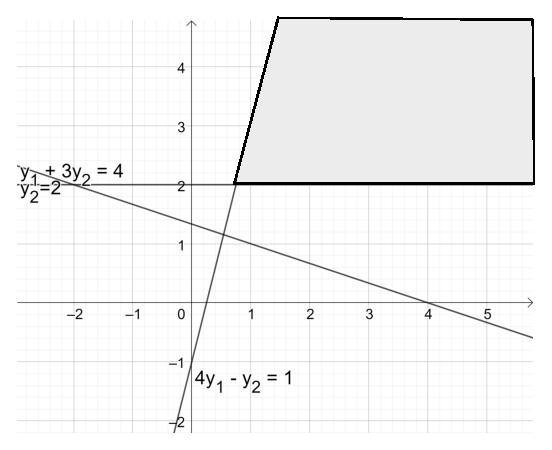
\includegraphics[width=160pt, height=160pt]{fig5.eps}
    \caption{Dualni problem: dopustiv region}
    \label{fig:fig5}
\end{figure}
Optimalno rješenje je u presjeku $y_2 = 3$ i $4y_1 - y_2 = 1$, i ono odgovara $y = (1, 3)$. Ispitajmo na osnovu komplementarnosti šta je optimalno rješenje problema (P). Imamo 
$$y_1 > 0 \Rightarrow (Ax - b)_1 y_1 = 0 \Rightarrow x_1 + 4 x_2 = 4 $$
$$y_2 > 0 \Rightarrow (Ax - b)_2 y_2 = 0 \Rightarrow 3x_1 - x_2 + x_2 = 3 $$
i kako je $y_1 + 3 y_2 > 4$, onda $(A^Ty)_1 > c_1$ i prema tome $x_1 =0$, 
odakle $x =(0, \frac{1}{4}, \frac{13}{4})$. 

\emph{Primjer.} Posmatrajmo problem LP-a:
$$\begin{array}{cccc}
   &\max                     &10 x_1 + 10 x_2 + 20 x_3 + 20 x_4  & \\
   &\mbox{s.t. }      &12 x_1 + 8 x_2  + 6 x_3  + 4 x_4   & \leq 210 \\
    &                        &3 x_1 + 6 x_2   + 12 x_3 + 24 x_4 & \leq 210 \\
     &                       & x_1,\ldots, x_4 \geq 0.                                 &
\end{array}
$$
Ovaj problem ima 4 varijable i 2 ograničenja. Prema tome, ima smisla razmatrati dualni problem  ($D$)  datog primala  ($P$)  jer u tom slučaju dobijamo linearno program od samo dvije varijable koji se može riješiti grafički.  ($D$)  problem je dat sa:

$$\begin{array}{ccc}
    &\min                    &  210 y_1 + 210 y_2      \\
    &\mbox{s.t. }     &  12 y_1  + 3   y_2 \geq 10 \\
    &                        &  8  y_1 + 6    y_2 \geq 10 \\
    &                        &  6 y_1 + 12 y_2  \geq 20 \\
    &                        &  4 y_1 + 24 y_2  \geq 20 \\
    &                        &  y_1, y_2 \geq 0.
\end{array}$$
Dopustiv region dualnog problema je dat na Slici~ \ref{fig:fig6-dual-region}. %gdje je dopustiv region označen plavom bojom. 
Dalje, može se pokazati da je optimum duala u presjeku prave $12 y_1 + 3 y_2 = 10$ i prave $6y_1 + 12 y_2 = 20$. Iz slike \ref{fig:fig6-dual-region} takođe vidimo da se druga i četvrta prava ne dostižu u tački optimuma (tu vrijedi stroga nejednakost nakon uvrštavanja tačke optimuma u uslove). Dakle, iz uslova komplementarnosti slijedi da za optimum $x$ primala  ($P$)  vrijedi $x_2 = 0$ i $x_4 = 0$.  Kako je $y_1, y_2 > 0$, onda vrijedi 

\begin{align}
    &10 x_1 + 20 x_3 = 210 \nonumber \\
    & 3x_1 + 12 x_3  = 210 \nonumber
\end{align}
odakle dobijamo rješenje $x_1 = 10, x_3 = 15$, pa je optimalno rješenje $x = (10, 0, 15, 0)$.

\emph{Zadatak}. Vrijednost 210 u drugom ograničenju u prethodnom problemu  ($P$)  zamijenite sa 421 i diskutujte optimalna rješenja  ($P$)  i  ($D$)  na sličan način kako je izvedeno  u datom primjeru.

\begin{figure}[!ht]
    \centering
    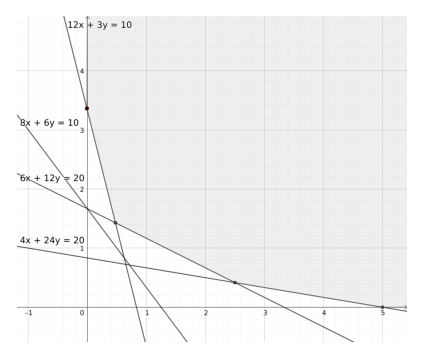
\includegraphics[width=170pt, height=170pt]{fig6.eps}
    \caption{Dopustiv region duala.}
    \label{fig:fig6-dual-region}
\end{figure}


\subsection{Metod Unutrašnje Tačke}

Simpleks metod ne garantuje   izvršavanje u polinomijalnom broju koraka u odnosu na veličinu ulaza. % V. Klee and G. Minty constructed an example LP: simplex method needs 2^n iterations to solve it 
Dakle, iz njega se ne može zaključiti da je problem rješavanja generalnog LP problema   polinomijalno rješiv. \emph{Metod unutrašnje tačke} će nam dati metod koji rješava ovu dilemu jer bilo koji LP problem može riješiti u polinomijanom vremenu, tj. pokazuje da je rješavanje problema LP-a pripada klasi $\mathcal{P}$. Iako u praksi često ne postiže dobre  performanse kao i simpleks metod, te se uvijek prvo preporučuje korištenje simpleks metoda u rješavanju LP-a, sa teoretskog stanovišta je veoma važan.  \emph{Metod unutrašnje tačke} (eng. Interior point metod) je dizajniran 50-ih godina XX vijeka i sve do 80-ih godina nije bio smatran za algoritam koji se efikasno može primijeniti na probleme velikih dimenzija. Tek 1984.godine (N. Karmakar, inžinjer u IBM-u) je formalno dokazao da se ovaj algoritam izvršava u polinomijalnom broju koraka za probleme linearnog programiranja. U današnje vrijeme, usljed ekstremnog poboljšanja performansi mašina, pokazao se da je \emph{metod unutrašnje tačke} kompetentan sa simpleks metodom kada je riječ o LP-u velikih dimenzija (sa matricom $A$ čiji je broj elemenata $10^9$ i više).

Za razliku od simpleks metoda, koji ``hoda'' po ivicama poliedra (dopustivog regiona), \emph{metod unutrašnje tačke}, kako i samo ime kaže, se kreće po unutrašnjim tačkama poliedra linearnog programiranja dok ne naiđe na optimalno rješenje problema. 

Postoji nekoliko metoda ove vrste, kao što su: metod centralne putanje, redukcija potencijala, afino skaliranje, itd. Mi ćemo u ovoj sekciji obratiti pažnju na metod centralne putanje. Da ponovimo, ova sekcija se bavi rješavanjem LP-a (\ref{eq:lp_equality_constraint}). 

Neka je dat par Primal-dual linearnih programa \\

$$ \begin{array}{lcc}
	&\mbox{Primal}            & \mbox{Dual}     \\
	&\min  c^T x       & \max  b^T y \\
	& \mbox{s.t.} Ax = b &   \mbox{s.t.} A^Ty + s = c \\
	& x \geq 0   &   s \geq 0
\end{array}
$$
Lagranžijan ovog para linearnih programa je dat sa 
\begin{equation}
	L(x,y) = c^Tx - y^T(Ax - b) - s^T x.
\end{equation}
Uslovi za nalazak stacionarne tačku Lagranžijana $L$ su dati sa:
\begin{align}
	&\triangledown_x L(x,y) = 0\\
	&\triangledown_y L(x,y) = 0
\end{align} 
što nas (uz uslov dualnosti) dovodi do uslova optimalnosti prvog reda za primal-dual par:
\begin{align}
	&Ax = b \\
	&A^T y + s = c \\
	&XS\mathbf{1} = 0 (x_j \cdot s_j =0 , \forall j) \\
	&  (x, s ) \geq 0,
\end{align}
gdje je $X = diag (x_1, \ldots, x_n)$, $S= diag(s_1,\ldots s_m)$, $\mathbf{1}=(1,\ldots, 1)$.

U nastavku navodimo problem preko koga razvijamo metod unutrašnje tačke. Ograničenja nenegativnosti u primalnom problemu ćemo zamijeniti sa $-ln x_j$. 
Primijetite da vrijedi 
$$\min e^{-\sum_{j=1}^n ln x_j} \Leftrightarrow \max \prod_{j} x_j $$
Dakle, minimizacija izraza $-\sum_{j=1}^n x_j$ je ekvivalentna maksimizaciji svih hiperravni koje definišu prvi ortant. Dakle, ovakav optimizacioni problem (na prvom ortantu) nas sprečava da se vrijednost neke od varijabli $x_j$ približi nuli (uprkos nenegativnim ograničenjima).  Na osnovu ovih činjenica, definišimo slejdeći optimizacioni problem. 

\begin{definition}
	Barijerni program LP-a (\ref{eq:lp_equality_constraint}) je dat u obliku 
	\begin{align*}
		&\min c^T x + \mu \sum_{j=1}^n ln(x_j) \\
		&\mbox{s.t. } A x = 0
	\end{align*}
\end{definition}
za neki $\mu >0$.
Sljedeću teoremu iz teorije optimizacije  za skalarne funkcije sa uslovnim ekstremima, koja je od bitne važnosti, navodimo je bez dokaza. 
\begin{thm}
	Neka skalarna funkcija  $f:\mathbb{R}^n \mapsto \mathbb{R}$ na skupu $g_1(x)=g_2(x)= \cdots = g_m(x) =0$ ima minimum u $x^*$. Onda vrijedi 
	$$ \triangledown f (x^*) = \sum_{i=1}^m y_i \triangledown g_i(x^*),$$
	gdje se $y_i$ nazivaju Lagranžovi množitelji. 
\end{thm}

Primijetimo da u problemu LP-a imamo sljedeće:
\begin{itemize}
	\item $f(x) = \min c^T x + \mu \sum_{j=1}^n ln(x_j) $;
	\item $g_i(x) = a_i x - b_i$.
\end{itemize}
Izračunajmo Lagranžove množitelje ovih funkcija. Vrijedi:

$$c + \mu (\frac{1}{x_1}, \frac{1}{x_2}, \ldots, \frac{1}{x_n}) = \Delta f (x) =\sum_{i=1}^m y_i \Delta g_i(x) = \sum_{i} y_i a_i = A^T y.$$ 

Uvedimo nenegativni vektor $s =\mu \cdot (\frac{1}{x_1}, \frac{1}{x_2}, \ldots, \frac{1}{x_n})$, pa imamo da bilo koje optimalno rješenje početnog problema treba da zadovoljava:
\begin{align}
	&A x = b \nonumber \\
	&A^T y + s = c  \nonumber \\
	& (s_1 x_1, \ldots, s_m x_m) = (\mu, \ldots, \mu) \label{eq:primal-dual-central-path-problem} \\
	& x, s \geq 0. \nonumber
\end{align}
Ovo nije linearni program, jer ograničenje 3 nije linearno.

\begin{definition}
	Primal-dual centralni put $\{(x(\mu), y(\mu), s(\mu)) \in \mathbb{R}^{2n + m} \mid \mu > 0 \}$ je rješenje koje zadovoljava uslove (\ref{eq:primal-dual-central-path-problem}) parametrizovano sa $\mu$. 
\end{definition}

Primijetimo sljedeće, ako se u problemu (\ref{eq:primal-dual-central-path-problem}) stavi $\mu = 0$, onda imamo 
\begin{align*}
	&(s_1 x_1, \ldots, s_m x_m) = (0, \ldots, 0) \\
	&\Longleftrightarrow s^T x = 0  \Longleftrightarrow (A^T y - c)^T x = 0 \\
	&\Longleftrightarrow y^T A x - c^T x = 0 \Longleftrightarrow y^T b = c^Tx
\end{align*}
jer je $Ax = b$. Primijetimo da   vrijednost (optimalnih) dualnih promjenjivih $y$ upravo odgovara vrijednosti Lagranžovih množitelja. Takođe, kako $\mu$ teži ka nuli, model (\ref{eq:primal-dual-central-path-problem}) sve preciznije aproksimira početni problem. 

Da bi došli do koraka samog algoritma, uvedimo notaciju 
$$ F(x, y, s) = \left (\begin{array}{c}
	Ax - b           \\
	A^T y + s - c     \\
	X S \textbf{1}                   
\end{array} \right ),$$
gdje je  $X = diag (x_1, \ldots, x_n ), S = diag(s_1,\ldots, s_n)$ i 
$\textbf{1} = diag (1,\ldots, 1)$. Primijetimo da je $X S \textbf{1}=\sum_{i} s_i x_i$. 
Potrebno je riješiti $F(x, y, s ) = 0, x,s \geq 0$. Korijen ove (nelinearne) jednačine ćemo naći uz pomoć \emph{Njutnovog metoda}. U nastavku u sažetom obliku izlažemo ideju Njutnovog metoda, jednog od najefikasnijih metoda za rješavanje ovakvih jednačina. Neka je data diferencijalna funkcija $f: \mathbb{R}^n \mapsto \mathbb{R}$.   Tangentna linija 
$$z - f(x^k) = \triangledown f(x^k) (x - x^k) $$
je lokalna aproksimacija grafa funkcije $f(x)$. Mijenjajući $z=0$, definiše se nova tačka 
\begin{equation} \label{eq:newton-step}
	x^{k+1} = x^k - (\triangledown f(x^k))^{-1} f(x^k).
\end{equation}
Pokazuje se da niz $\{x^k\}_{k \in \mathbb{N}}$ definisan uz pomoć (\ref{eq:newton-step}) konvergira ka stacionarnoj tački funkcije $f(x)$. Simulacija koraka njutnovog metoda je data na Slici~\ref{fig:newton}. 

\begin{figure}[!ht]
	%    \centering
	\begin{tikzpicture}[thick,yscale=0.6,xscale=0.8]
		
		% Axes
		\draw[-latex,name path=xaxis] (-1,0) -- (12,0) node[above]{\large $x$};
		\draw[-latex] (0,-2) -- (0,8)node[right]{\large $y$};;
		
		% Function plot
		\draw[ultra thick, orange,name path=function]  plot[smooth,domain=1:9.5] (\x, {0.1*\x^2-1.5}) node[left]{$f(x)$};
		
		% plot tangent line
		\node[violet,right=0.2cm] at (8,4.9) { tangenta};
		
		\draw[gray,thin,dotted] (8,0) -- (8,4.9) node[circle,fill,inner sep=2pt]{};
		\draw[dashed, violet,name path=Tfunction]  plot[smooth,domain=4.25:9.5] (\x, {1.6*\x-7.9});
		
		% x-axis labels
		\draw (8,0.1) -- (8,-0.1) node[below] {$x^{k}$};
		\draw [name intersections={of=Tfunction and xaxis}] ($(intersection-1)+(0,0.1)$) -- ++(0,-0.2) node[below,fill=white] {$x^{k+1}$} ;
	\end{tikzpicture}
	\caption{Njutnova metoda u ravni.}
	\label{fig:newton}
\end{figure}
%\begin{figure}[!ht]
%    \centering
%    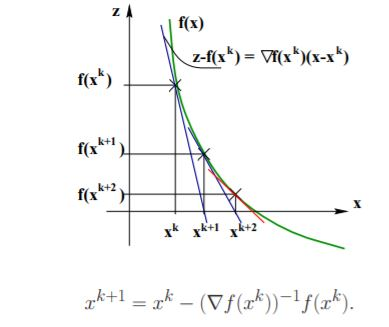
\includegraphics[width=170pt,height=170pt]{newton.jpg}
%    \caption{Demonstracija njutnovog metoda u ravni.}
%    \label{fig:newton}
%\end{figure}

Primijenimo ovu metodu na nalaženje nule funkcije $F(x,y,s)$. Tada imamo
$$ \triangledown F =\left ( \begin{array}{ccc}
	A   & 0      &  0      \\
	0   & A^T    &  I      \\
	S   & 0      & X       \\
\end{array} \right ) 
$$
Prema tome, u tački $(x,y,s)$, Njutnov pravac
$
\begin{pmatrix}
	\bigtriangleup  x  \\
	\bigtriangleup  y  \\
	\bigtriangleup  s  \\
\end{pmatrix}
$
%$\bigtriangleup x = x^{k+1} - x^{k}, \bigtriangleup y = y^{k+1} - y^{k}, \bigtriangleup s = s^{k+1} - s^{k}$
se izračunava rješavajući sistem linearnih jednačina:

\begin{equation}
	\begin{pmatrix}
		A   & 0      &  0      \\
		0   & A^T    &  I      \\
		S   & 0      & X       \\
	\end{pmatrix}  
	\begin{pmatrix} 
		\bigtriangleup  x  \\
		\bigtriangleup  y  \\
		\bigtriangleup  s  \\
	\end{pmatrix} 
	= 
	\begin{pmatrix} 
		b - Ax             \\
		c - A^T y - s      \\
		- X S \textbf{1}  \\                   
	\end{pmatrix} 
\end{equation}

Njutnov metod pod punim brojem iteracija obično narušava uslove $x,s \geq 0$, ali to se može izbjeći (biće prikazano u nastavku).  
Prethodno izloženo se može lako proširiti i na slučaj kada ne vrijedi $s_ix_i = 0$, tj. kada je $\frac{1}{n}s_ix_i = \mu, \mu > 0$, $i=1,\ldots,n$. Na sličan način računamo Njutnov pravac u smijeru $s_i x_i \approx \mu \theta$, za  $\theta >0$, iz sistema 

\begin{equation} \label{eq:newton-interior-system-k}    
	\begin{pmatrix}
		A   & 0      &  0      \\
		0   & A^T    &  I      \\
		S   & 0      & X       \\
	\end{pmatrix} 
	\cdot 
	\begin{pmatrix}
		\bigtriangleup  x  \\
		\bigtriangleup  y  \\
		\bigtriangleup  s  \\
	\end{pmatrix} 
	=
	\begin{pmatrix}
		b - Ax           \\
		c - A^T y - s      \\
		\theta \mu \mathbf{1} - X S \textbf{1}                      
	\end{pmatrix}
\end{equation}

%https://www.youtube.com/watch?v=Zf_bn3jJFKY&list=WL&index=9&t=647s
\emph{Algoritam unutrašnje tačke} se sastoji od sljedećih koraka:
\begin{enumerate}
	\item Inicijalizujemo $k=0$, te proizvoljno  $(x^k, y^k, s^k), x^k, s^k \geq 0$, $x^k,s^k \in \mathbb{R}^n, y^k \in \mathbb{R}^m$.
	\item Izaberimo $ \theta^k \in [0, 1]$ te riješimo sistem (\ref{eq:newton-interior-system-k}) za $(x^k,y^k,s^k)$ i odabran $\theta_k$ te $\mu^k = (y^k)^T s^k $, za neko odakle   dobijamo
	$  
	\begin{pmatrix}
		\bigtriangleup x^k      \\
		\bigtriangleup y^k       \\
		\bigtriangleup s^k       \\
	\end{pmatrix}    
	$
	
	\item $ 
	\begin{pmatrix}
		x^{k+1}  \\
		y^{k+1}   \\
		s^{k+1}   \\
	\end{pmatrix} \approx
	\begin{pmatrix}
		x^k  \\
		y^k  \\
		s^k  \\
	\end{pmatrix} +   
	\alpha_k 
	\begin{pmatrix}
		\bigtriangleup x^k       \\
		\bigtriangleup y^k       \\
		\bigtriangleup s^k       \\
	\end{pmatrix}  
	$, gdje je $\alpha_k$ izabran na taj način da $(x^{k+1}, s^{k+1}) > 0$, tj. da bi se očuvala dopustivost rješenja. 
	\item Ažurirajmo $k = k + 1$, te se vratimo na korak 2.
\end{enumerate}
Primijetimo da $\mu \rightarrow 0$, kako $k \rightarrow \infty$. U praksi se često stavlja $\theta^k = 1 - \frac{\beta}{n}$, za $\beta \in (0,1)$, a najčešće $\beta= 0.1$.  Parametar $\beta$ upravlja brzinom progresa prema optimalnom rješenju.  


Može se pokazati sljedeća teorema koja karakteriše \emph{metod unutrašnje tačke}.

\begin{thm}
	\begin{itemize}
		\item Algoritam unutrašnje tačke konvergira ka optimalnom rješenju problema (\ref{eq:lp_equality_constraint}). %Dualna granica se smanjuje $1 - \frac{\beta}{n}$ pri svakom koraku.
		\item U svim iteracijama, algoritam generiše dopustive tačke.
		\item Kompleksnost algoritma je $O(\sqrt{n})$. Dakle,  broj iteracija koji je proporcionalan $\sqrt{n}$ će biti potreban da algoritam riješi problem. 
	\end{itemize}
\end{thm}

% dualni simpleks metod ==> 4.7 PRIMAL-DUAL ALGORITHMS
 
\newpage

\section{Cjelobrojno Programiranje}

%https://www.google.com/url?sa=t&source=web&rct=j&url=https://web.mit.edu/15.053/www/AMP-Chapter-09.pdf&ved=2ahUKEwiN0cef_f7xAhU0CRAIHWLqCw0QFjAfegQILBAC&usg=AOvVaw1cQCbZJQbc55Z0VLPue2ul
Ponekad nije realno očekivati da varijable odluke dobijaju neprekidne vrijednosti. Recimo, ako se zahtjeva u rasporedu u smjenama da dovoljan broj ljudi bude u svakoj od smjena. Ovaj broj je cjelobrojan, preciznije prirodan broj. U slučaju da su sve varijable odluke u modelu problema cjelobrojne, riječ je o problemu cjelobrojnog programirnja (eng. \emph{Integer programming}). 
U ovom odjeljku ćemo se pozabaviti linearnim cjelobrojnim programiranjem (ILP) gdje se zahtjeva da funkcija cilja kao i ograničenja u modelu budu linearni u varijablama. Prema tome ILP ima opšti oblik:
\begin{align}
    & \max c^T x \nonumber\\
    & A x \leq b \nonumber \\
    & x \geq 0 \nonumber\\
    & x_i \in \mathbb{Z}, \mbox{ za sve } i \label{ilp-formulation}
\end{align}
U nastavku modelujmo još nekoliko problema pomoću paradigme ILP-a.

\subsection{Neki problemi modelovani pomoću ILP-a}

\emph{Problem ruksaka.} Neka je dato $n$ proizvoda i neka je težina $i$-tog proizvoda jednaka $w_i$, dok je vrijednost $c_i$, $i=1,\ldots,n$. Koje proizvode treba da stavimo u ruksak kapaciteta $C$ tako da je vrijednost proizvoda u ruksaku maksimalna. \\
\emph{Rješenje}. Definišimo varijable $x_i$ koje dobijaju vrijednost 1 ako odaberemo $i$-ti proizvod, u protivnom je 0, $i=1,\ldots,n$. Ograničenje kapaciteta ruksaka se modeluje ograničenjem $\sum_{i=1}^n w_i x_i \leq C$, dok je funkcija cilja ta koja maksimizujem profit odabranih proizvoda, dakle modeluje se uz pomoć linearne kombinacije $f(x) = \sum_{i=1}^n c_i x_i$. Time smo modelovali ovaj problem.

\emph{Problem rasporeda}. Čitava klasa problema koja se naziva sekvenciranje, raspoređivanje i usmjeravanje u osnovi su predstavljeni modelima cjelobrojnog programiranja. Kao primjer, recimo da je potrebno rasporediti studenate u  učionicu na takav način
da je minimizovan broj učenika koji ne mogu pohađati nastavu koja je njihov prvi izbor među ostalim. Postoje ograničenja u pogledu broja i veličine učionica dostupnih u bilo kom trenutku, dostupnosti predavača na fakultetu u određeno vrijeme i preferencijama studenata za određene rasporede. Jasno je da imam varijablu za svakog $i$-ti studenta 
za $j$-to predavanje tokom $n$-tog vremenskog perioda (recimo vrijeme je diskretizovano po 45 min/čas) -- koja je jednaka 1 ako se student uklapa u takav raspored, inače 0. 

Posmatrajmo ipak malo specifičniji problem u odnosu na ovaj generalni (koji je dosta težak i za modeovanje, a kamoli za rješavanje). 
Razmotrimo raspoređivanje osoblja zaduženog za upravljanje letom aviona. 
Avionska kompanija mora rasporediti svoje osoblje na rutama koje pokrivaju sve letove. Treba paziti, na primjer, da jedna posada treba da upravlja letom iz  Beograda u Zagreb (u 10:00), a takođe letom iz Zagreba u Cirih (u 14:00). Dakle, jedna posada treba da je uključena u rutu na kojoj upravlja različitim letovima. Prema tome, raspoređujemo posadu na rutu $j$, modelovana uz pomoć binarne varijable 
$$x_j = \begin{cases}
    &1, \mbox{ ako je barem jedna osoba prodružena ruti} j \\
    &0, \mbox{inače}. 
\end{cases}
$$
Dalje, definišimo 
$$a_{ij}= \begin{cases}
             &1, \mbox{ ako je let } i \mbox{ pridružen ruti } j \\
             & 0, \mbox{ inače}.
        \end{cases}
$$
Neka je $c_j$ cijena dodjeljivanja neke posade ruti $j$. Ovdje $a_{ij}$ definišu prihvatljive kombinacije letova sa rutama, uzimajući u obzir  karakteristike kao što su redoslijed krakova za uspostavljanje veza između letova i za uključivanje u rute osnovno vrijeme  održavanja leta (iskrcavanje, istovaranje kofera, utovaranje novih kofera, ukrcavanje itd.).  

Model postaje 
\begin{align}
    &\min \sum_{i=1}^n c_j x_j \nonumber\\
    & \sum_{j=1}^n a_{ij} x_j \geq 1, \forall i \in \{1,\ldots, m\} \label{ineq:set_cover} \\
    & x_i \in \{0, 1 \},, \forall i \in \{1, \ldots, n\} \nonumber
\end{align}
Ograničenje (\ref{ineq:set_cover}) je poznato ograničenje koje se javlja u pokrivanju problema skupa (eng. \emph{set-covering problem}).

\emph{Problem trgovačkog putnika}. Problem ima ovakvu formulaciju: krenuvši od svog mjesta, putnik želi da posjeti ostalih ($n-1$) gradova pod minimalnim troškovima. U suštimi, ovo je grafovski problem gdje je ulaz (bez smanjenja opštosti) kompletan težinski graf, a gdje je potrebno naći hamiltonovu konturu minimalne težine u datom grafu. Pod težine konture se podrazumijeva zbir težina njenih grana. 

\emph{Rješenje}. Označimo težinu grane od grada $i$ do grada $j$ sa $c_{ij}$.  Definišimo (binarne) varijable 
$$x_{ij} = \begin{cases}
                1, \mbox{ ako putnik u svojoj ruti iz grada } i \mbox{ posjeti grad } j \\
                0, \mbox{ inače}. 
          \end{cases}$$ 
Potrebno je nametnuti sljedeća ograničenja -- svaki grad se treba naći u ruti,  što možemo postići sa 
$$  \sum_{i=1}^n x_{ij} = 1, \forall j =1,\ldots, n,$$ 
što znači da se iz tačno jednog grada dolazi u svaki grad $j$, dok sličnim jednakostima nametnemo da se iz grada $j$ odlazi u tačno jedan drugi grad sa:

$$  \sum_{j=1}^n x_{ij} = 1, \forall i =1,\ldots, n$$ 
 uz uslove $x_{ij}\geq 0$. Primijetimo sljedeće, ovakvi uslovi ne sprečavaju pojavu rješenja koja predstavljaju uniju disjunktnih podruta, što nije dopustivo u našem slučaju. Ako pretpostavimo da je rješenje dato u obliku podruta $R_1, \ldots, R_k$, gdje je $R_i = \{ v_{i_1}, \ldots, v_{i_k} \}$, onda se može izbjeći pojava podruta dodavanjem dodatnih ograničenja u početni model problema. Recimo, eliminacija pojave podrute $R_2$ (u odnosu na podrutu $R_1$) se vrši dodavanjem ograničenja:
 $$ \sum_{l=1}^{1_k}\sum_{t=1}^{2_k} x_{1_l, 2_t} \geq 1.$$
 U najgorem slučaju, potrebno je dodati $2^n-1$ ovakvih ograničenja. 
 
 \subsection{Neke tehnike konstrukcije modela Cjelobrojnog Programiranja}
 
 \emph{Binarne varijable.} Pretpostavimo da trebamo odrediti da li uključiti sljedeće aktivnosti: ($i$) izgraditi novo postrojenje,
($ii$) poduzeti reklamnu kampanju ili ($iii$) razviti novi proizvod. Jasno je da su ove odluke korespondiraju ka logičkim odlukama da ili ne, prema tome modelujemo ih sa  $x_i \in \{0, 1 \}$, i=1,2,3. Često se nameće uslov da se najviše jedna od odluka izvrši, što se modeluje sa $\sum_{i=1}^3 x_1 \leq 1$. Ovo ograničenje se obično naziva \emph{ograničenjem sa višestrukim izborom} (eng. multiple--choice constraint), jer se njime ograničava izbor odluka na najviše jednu od, u ovom slučaju, tri dostupne alternative. 


Pretpostavimo da proizvođač lijekova mora da odluči hoće li koristiti spremnik za fermentaciju. Ako koristi spremnik, tehnologija obrade zahtijeva da se napravi $X$ jedinica ljekova. Dakle, proizvodnja $y$ mora biti 0 ili $K$, a problem se može modelirati binarnom varijablom $x_j \in \{ 0, 1\}$ zamjenom $Kx_j$ za $y_i$. 

\emph{Logička ograničenja}. Jedno od najprostijih logičkih pitanja u matematičkom programiranju je da li dati izbor varijabli odluka zadovoljava ograničenje, ili da li je generalno ograničenje

\begin{equation}\label{eq:constr-ex-1-ilp}
   f(x_1,\ldots, x_n )\leq b
\end{equation}
 zadovoljeno?
 
 Uvedimo binarnu varijablu $y$ na sljedeći način:
 
$$y =\begin{cases}
1, \mbox{ ako je poznato da je ograničenje zadovoljeno}, \\
0, \mbox{ inače}
\end{cases}$$
te napišimo 
\begin{equation}\label{eq:constr-ex-1-ilp-big-B}
   f(x) - M y \leq b,
\end{equation}

gdje je $M$ konstanta tako da je 
ograničenje zadovoljeno za sve $x$ ako je $y =1$. Kad god je $y=0$ i ako je uslov (\ref{eq:constr-ex-1-ilp}) zadovoljen, onda je i ograničenje (\ref{eq:constr-ex-1-ilp-big-B}) zadovoljeno. U praksi je određivanje konstante $B$ često vrlo jasno iz samog problema. Inače, veoma je bitno da uzmemo što manju vrijednost za $M$ da bismo izbjegli potencijalne numeričke probleme prilikom računanja. 

\emph{Alternativna ograničenja}. Pogledajmo sljedeću situaciju sa alternativnim ograničenjima:
\begin{align}
     &f_1(x) \leq b_1 \vee \nonumber\\
     &f_2(x) \leq b_2.\label{ineq:f_leq_b2}
\end{align}
gdje je u modelu traženo da se zadovolji barem jedno od ograničenja. 
Ovo ograničenje se može dobiti kombinovanjem logičkih ograničenja te ograničenja sa višestrukim izborom. Dakle, imamo 
\begin{align*}
      &f_1(x) - M_1 y_1  \leq b_1 \\
      &f_2(x) - M_2 y_2  \leq b_2 \\
      & y_1 + y_2 \leq 1 \\
      & y_1, y_2 \in \{0, 1\}.
\end{align*}
Konstante $M_1$ i $M_2$ se odabiru da oba ograničenja u (\ref{ineq:f_leq_b2})  budu (trivijano) zadovoljena, te time postanu invarijante kad je $y=1$.

Ograničenje $y_1 + y_2 \leq 1$ implicira da barem jedna od $y$--varijabli mora da bude 0, tj. barem jedno ograničenje mora da bude zadovoljeno. 

Primijetimo da možemo  pojednostaviti ovu formulaciju koristeći $y_1 - y_2 = 1$ (jer ovo povlači da ili $y_1$ ili $y_2$ su 0), tj. uvrštanjem $y_2 =  1-y_1$, odakle dobijamo 
\begin{align*}
      & f_1(x) - M_1 y_1       \leq b_1 \\
      & f_2(x) - M_2 (1-y_1)   \leq b_2  \\
      & y_1, y_1 \in \{0,1 \}.
\end{align*}
\emph{Uslovna ograničenja}. 
Pretpostavimo da želimo modelovati sljedeći scenario sa ograničenjima 
\begin{align*}
    f(x) > b_1 \Rightarrow f(x) \leq b_2 
\end{align*}
Kako je implikacija $p \Rightarrow q$ ekvivalentna sa $\neg p \wedge q$, pa prema tome imamo da je scenarion ekvivalentan sa
\begin{align*}
    f(x) \leq b_1 \vee f(x) \leq b_2 
\end{align*}
odakle sijedi da koristeći alternativna ograničenja možemo da modelujemo uslovna ograničenja.

\emph{K-alternative}. Pokušajmo da modelujemo scenario da od $m$ ograničenja
$$f_j(x) \leq nb_j, j=1,\ldots,m,$$
barem $k$ od njih treba da budu zadovoljena. Modelovanje ovakvog scenarija vršimo na način da prvo odredimo konstante koje će ignorisati ograničenja, nazovimo ih $M_1, \ldots, M_m$, redom. generalni problem u tom slučaju može biti definisan na sljedeći način:
\begin{align}
     &f_j(x) + (1-y_j) M_j \leq b_j, j=1,\ldots,m\\
     & \sum_{i=1}^m y_i \geq k \\
     & y_j \in \{0,1\}, j=1,\ldots,m.
\end{align}
Primijetimo da ako je $y_j = 1$, tada je $j$-to ograničenje zadovoljeno (za dato $x$). Dakle, barem $k$ ograničenja treba da budu zadovoljena da bi $x$ bilo dopustivo rješenje. 

\emph{Složene alternative}. Pretpostavimo da se region sastoji od tri disjunktna regiona kao na Slici~\ref{fig:compound_regions}. Ovakav scenario se može modelovati uz pomoć konstante veliko $M$, te  ograničenjem sa višestrukim izborom dobijamo:
\begin{align*}
    &f_1(x) - M_1 y_1 \leq b_1 \\
    &f_2(x) - M_2 y_2 \leq b_2 (\mbox{region 1}) \\ \hline
    & f_3(x) - M_3 y_3 \leq b_3 \\ 
    & f_4(x) - M_4 y_4 \leq b_4 (\mbox{region 2})\\  \hline 
    & f_5(x) - M_5 y_5 \leq b_5 \\
    & f_6(x) - M_6 y_6 \leq b_6 \\
    & f_7(x) - M_7 y_7 \leq b_7 (\mbox{region 3}) \\ \hline
    & y_1 + y_2 + y_3 \leq 2 \\
    & x_1, x_2 \geq 0 \\
    & y_1, y_2, y_3 \geq 0.
\end{align*}

\begin{figure}[!ht]
    \centering
    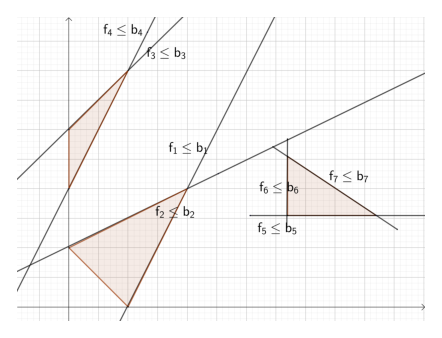
\includegraphics[width=200pt, height=200pt]{compound.eps}
    \caption{Dopustiv region sa više disjunktnih regiona.}
    \label{fig:compound_regions}
\end{figure}
Uslov $y_1 + y_2 + y_3 \leq 2$ nam upravo ograničava da rješenje $(x_1, x_2)$ pripada tačno jednom od (disjunktnih) dopustivih regiona. 

\emph{Reporezentovanje nelinearnih funkcija}. ($i$) \underline{Fiksne cijene}. Ciljna funkcija problema minimizacije može da sadrži i neke fiksne troškove (fiksni troškovi ulaganja, fiksni troškovi postavljanja opreme itd.). Na primjer, trošak proizvodnje $x$ jedinica određenog proizvoda može da se sastoji od fiksnih troškova postavljanja opreme i promjenjivih troškova koji se tiču proizvedene robe na opremi (mašinama). Pretpostavimo da oprema ima kapacitet proizvodnje od $B$ jedinica. Neka je $y$ binarna varijabla koja pokazuje kada nastaje fiksni trošak, pri čemu  je $y=1$ ako je $x >0$, dok je $y=0$ ako je $x=0$. Tada doprinos cijeni proizvodnje $x$ jedinica proizvoda ima oblik 
$$ yB + c x $$ pod uslovima:
\begin{align}
     &x \leq By \\
     & x \geq 0 \\
     & y \in \{0, 1\}.
\end{align}
Primijetimo da je ovaj model pripada modelima \emph{Mješovitog-cjelobrojnog programiranja} (gdje postoje obje vrste varijabli, neprekidne i cjelobrojne). O ovoj paradigmi će biti više riječi u narednim sekcijama. \\
($ii$) \underline{{Po dijelovima linearna funkcija}}. Druga vrsta nelinearne funkcije koja se može predstaviti cjelobrojnim varijablama je po-dijelovima-linearna funkcija. Radi jednostavnosti, posmatramo takve funkcije u ravni. To znači da funkcija sama po sebi nije linearna, ali kada joj se domen rastavi na komade (intervale), ona postaje linearna na svakom od tih komada. Recimo da se ova funkcija sastoji od tri po dijelovima (nezavisne) linearne funkcije, tj. 
$$f(x) = \begin{cases}
          c_1 x, \mbox{ za } x \in I_1 = [\delta^1_1, \delta^1_2] \\
          c_2 x, \mbox{ za } x \in I_2 = [\delta^1_2 = \delta^2_1, \delta^2_2] \\
          c_3 x, \mbox{ za } x \in I_3 = [\delta^2_2 = \delta^3_1, \delta^3_2].
      \end{cases}
$$
gdje su $I_1, I_2$ i $I_3$ disjunktni intervali na $\mathbb{R}$.

Da bi se modelovala funkciju cilja modela, varijablu $x$ izrazimo na osnovu tri varijable 
$$x = \beta_1 + \beta_2 + \beta_3$$
pod uslovima 
\begin{align}
     &0   \leq \beta_1 \leq \delta^1_2 - \delta^1_1 = b_1 \nonumber \\
     &0  \leq \beta_2 \leq \delta^2_2 - \delta^2_1 = b_2 \nonumber \\
     &0  \leq \beta_3 \leq \delta^3_2- \delta^3_1 = b_3, \label{eq: piecewise-constraints}
\end{align}
te je cijena tada jednaka 
$$ C = c_1 \beta_1 + c_2 \beta_2 + c_3 \beta_3.$$ 
Primijetimo da imamo problema na graničnim uslovima intervala, dakle u tačkama $I_1 \cap I_2 =\{\delta^1_2\}$ i $I_2 \cap I_3 =\{\delta^2_2\}$. Trebalo bi da vrijedi da $\beta_1 =  \delta^1_2 - \delta^1_1$ kad god je $\beta_2  > 0$ kao i $\beta_2 =  \delta^2_2 - \delta^2_1$ kad god je $\beta_3  > 0$.  S obzirom da su ovo uslovna ograničenja, ona se modeluju uvođenjem dodatnih binarnih varijabli 
$$ \omega_1 = \begin{cases}
                   1, \mbox{ ako } \beta_1 \mbox{ dostiže svoju gornju granicu} \\
                   0, \mbox{ inače},
              \end{cases}$$
te 
$$ \omega_2 = \begin{cases}
                   1, \mbox{ ako } \beta_2 \mbox{ dostiže svoju gornju granicu} \\
                   0, \mbox{ inače}, 
              \end{cases}$$
pa se ograničenja u (\ref{eq: piecewise-constraints}) mogu napisati u obliku

\begin{align}
     & b_1 \omega_1 \leq \beta_1 \leq  \leq b_1   \nonumber \\
     & b_2 \omega_2 \leq \beta_2 \leq \omega_1 b_2 \nonumber \\
     & 0 \leq \beta_3 \leq b_3 \omega_2 \nonumber \\
     & \omega_1, \omega_2 \geq 0. \label{eq: piecewise-constraints-equivalent}
\end{align}
      Primijetimo da ako $\omega_1 = 0$, onda je $\omega_2= 0$ kako bi se održala dopustivost za ograničenja nametnutog od strane $\beta_2$, pri čemu se uslovi u (\ref{eq: piecewise-constraints-equivalent}) prevode u
      $$ 0 \leq \beta_1 \leq b_1, \beta_2 =0, \beta_3 =0.$$
      Ako je $\omega_1 = 1, \omega_2 = 0$, onda se uslovi u (\ref{eq: piecewise-constraints-equivalent}) prevode u
            $$   \beta_1 = b_1, 0 \leq \beta_2 \leq b_2, \beta_3 =0.$$
    Ako je $\omega_1 = \omega_2 = 1$, onda se  uslovi u (\ref{eq: piecewise-constraints-equivalent}) prevode u
    $$ \beta_1 = b_1, \beta_2 = b_2, 0 \leq \beta_3 \leq b_3.$$
    Prema tome, postoje 3 dopustive kombinacije parametara $\omega_1$ i $\omega_2$:
    \begin{itemize}
             \item  $\omega_1 = 0, \omega_2= 0:$ koje odgovara $x \in I_1$ jer $\beta_2=\beta_3=0$;  
             \item $\omega_1 = 1, \omega_2 = 0$: koje odgovara $x\in I_2$, jer je $\beta_1=b_1, \beta_3=0$;
              \item $\omega_1 = 1, \omega_2 = 1$: koje odgovara $x\in I_3$, jer je $\beta_1=b_1, \beta_2=b_2$.
    \end{itemize}
    
\emph{Aproksimacija nelinearnih funkcija}. Ako je funkcija cilja nelinearna, ona se aproksimira pomoću niza po-dijelovima-linearnih funkcija, pa se onda primjenjuje transformacija ograničenja u modelu objašnjena u prethodnom. 

Da bi objedinili većinu gore navedenih transformacija ograničenja, posmatrajmo sljedeći primjer. 


\emph{Primjer}. Pretpostavimo da je stanovništvo koncentrirano u $I$ okruga  unutar grada i da u okrugu $i\in [I]$ ima $p_i$ ljudi. Preliminarna analiza (premjeri zemljišta, politika, socijalna situacija, itd.) ograničila je potencijalnu lokacije vatrogasnih domova na $J$ mjesta. Neka je $d_{ij} \geq 0$ udaljenost od središta okruga $i$ do mjesta $j$. Zadatak je da se nađe najbolji odabir mijesta gdje će se dodijeliti vatrogasni domovi u okruzima. 

Definišimo binarne varijable 
$$y_i = \begin{cases}
              1, \mbox{ ako je mjesto } i \mbox{ odabrano} \\
              0, \mbox{ inače}
        \end{cases}$$
i 
$$
x_{ij}= \begin{cases}
             1, \mbox{ ako je okrug } i \mbox{ pridružen mjestu } j \\
             0, \mbox{ inače}. 
        \end{cases}
$$
Svaki okrug treba da bude pridružen tačno jednom vatrogasnom domu, pa je to ograničenje modelovano sa
\begin{equation}\label{eq:ex-constr-1}
      \sum_{j \in J} x_{ij} = 1, \forall i \in I
\end{equation}
Takođe, ne postoji okrug koji je pridružen nekorištenom mjestu (za vatrogasni dom) $j$, tj. ako je $y_j = 0$, onda $ \sum_{i \in I} x_{ij} = 0$. Ovo je uslovno ograničenje, koje se modeluje sa
\begin{equation}\label{eq:ex-constr-2}
    \sum_{i \in I} x_{ij} \leq y_j |I|,
 \end{equation}
gdje je $|I|$ broj mijesta. 

Dalje, udaljenost od okruga $i$ ka njegovom pridruženom vatrogasnom domu je jednaka $d_i = \sum_{j} d_{ij}x_{ij} $. Dalje, populacija koja će biti servisirana od strane mjesta $j$ je jednaka 
\begin{equation}\label{eq:ex-constr-3}
    s_j = \sum_{i} p_i x_{ij}. 
\end{equation}
Pretpostavimo da je središnji okrug posebno osjetljiv na požar i da ili mjesta 1 i 2 ili mjesta 3 i 4 mogu biti iskorištena da zaštite okrug. Ovakva situacija se modeluje sa
\begin{equation*} 
    y_1 + y_2 \geq 2 \mbox{ ili } y_3 + y_4 \geq 2
\end{equation*}
što je ekvivalentno ograničenjima 
\begin{align}
    &y_1 + y_2 \geq 2 y \nonumber \\
    &y_1 + y_2 \geq 2 (1-y) \nonumber \\
    & y \in \{0, 1 \}.\label{eq:ex-constr-4}
\end{align}
Pretpostavimo da cijena izgradnje vatrogasnog doma na mjestu $j$ koje može servisirati $s_j$ ljudi košta $f_j(s_j)$. Pretpostavimo takođe da je budžet kojim raspolažemo jednak $B$. Prema tome, vrijedi ograničenje
\begin{equation}\label{eq:ex-constr-5}
     \sum_{j \in J} f_j(s_j) \leq B.
\end{equation}
 Funkcija cilja koja bi se mogla optimizovati je minimizacija udaljenosti 
 okruga koja je najdalje od svog pridruženog vatrogasnog doma ($d_i$):
      $$\min D $$
 gdje je $D= \max d_i$. Ekvivalentno se ova funkcija cilja napiše kao:
 \begin{align*}
      &\min D \\
      & D \geq d_i,  \forall i \in I
      & \mbox{s.t. } (\ref{eq:ex-constr-1})--(\ref{eq:ex-constr-5}).
 \end{align*}
 Još je ostalo zamijeniti svaku funkciju $f_j (s_j)$ aproksimacijom cjelobrojnog programiranja kako bismo dzavršili modeliranje. Detalje ostavljamo kao zadatak. Ako bi funkcija $f_j (s_j)$ sadržala fiksne troškove, tada se ne bi trebale uvoditi nove varijable fiksnih troškova -- u tu svrhu služi već uvedena varijabla $y_j$. 
 
 \newpage 
 \section{Tehnike rješavanja problema Cjelobrojnog programiranja}
 
 Dok je simpleks metoda učinkovita za rješavanje  problema LP-a, ne postoji jedinstvena tehnika za rješavanje problema Cjelobrojnog programiranja. Umjesto toga, razvijeni su mnogi postupci i njihova efikasnost
 uvelike zavisi od samog problema. Dosadašnje metode se generalno mogu klasifikovati na sljedeći način:
 \begin{enumerate}
     \item Enumerativne tehnike -- Dinamičko programiranje, metoda otkidanja i ograničavanja (eng. \emph{branch-and-bound}), koju ćemo kratko zvati B\&B;
     \item Tehnike otkidajućih ravni;
     \item Grupne-teoretske tehnike. 
 \end{enumerate}

U osnovi, mi ćemo se baviti sa prve dvije vrste metoda. Za model ILP-a (\ref{ilp-formulation}), zanemarujući uslov da varijable treba da budu cjelobrojne (već da uzimaju realne, pozitivne vrijednosti), dobijamo tzv. odgovarajucu LP \emph{relaksaciju} ILP-a (\ref{ilp-formulation}). LP relaksacija se može vrlo lako riješiti uz pomoć simpleks metoda pri čemu dobijemo rješenje $x^*$. Posmatrajući vektor $\overline{x}$ koje se dobijaju zaokružujući svaku od vrijednosti koordinata vektora $x^*$ na njenu najbližu cjelobrojnu, dobijamo cjelobrojni vektor iz LP-a. Međutim, iako je uslov o cjelobrojnosti (kakav je u odgovarajućem ILP-u potreban) ispunjen, može se desiti da ovakvo rješenje izvedeno iz LP relaksacije problema (\ref{ilp-formulation}) ne mora da bude dopustivo. Ali, u osnovi, skaliranjem desnih strana ILP-a kao i koeficijenata funkcije cilja na odgovarajući način, moguće je konstruisati probem čije je optimalno cjelobrojno rješenje udaljeno koliko želimo od zaokruženog rješenja LP relaksacije. Ovim ćemo se baviti u nastavku. 

\subsection{Metoda grananja i ograničavanja (B\&B)}
B\&B tehnika programiranja je zasnovana na principu ``zavadi pa vladaj'' gdje se problem rastavlja na manje dijelove, i tako rekurzivno (ako je potrebno). Kasnije se (optimalna rješenja) manjih problema kombinuju za dobijanje optimalnog rješenja početnog problema.  U B\&B strategiji dodatak je da se 
problem ne rastavlja na manje podprobleme ako se uspostavi da je rješenje podoptimalno (lošije od trenutno najboljeg dopustivog rješenja). U rješavanju ILP-a, dopustiv skup se dijeli na manje skupove, i tako rekurzivno (ako je potrebno) dok se ne dobiju podproblemi koji su trivijalo rješivi. Svi ovakvi B\&B pristupi se razlikuju u načinu podjele dopustivog skupa i zbog toga ih postoji nekoliko različitih u literaturi. 

\subsubsection{Bazni B\&B za rješavanje problema ILP-a}

Navedimo sljedeće bitne stavke koje vrijede:
\begin{itemize}
    \item  U LP relaksaciji u problemu 
           maksimizacije, optimalna vrijednost funkcije cilja 
           uvijek će biti gornja granica (UB) posmatranog ILP-a. 
    \item  Bilo koja cjelobrojna tačka LP relaksacije na nekom podskupu  
           dopustivog skupa uvijek je  donja granica (LB) optimalne vrijednosti početnog ILP-a. 
\end{itemize}
Definišimo $LB = - \infty$. 
Bazirani na ove dvije činjenice, uvedimo sistematičnu podjelu dopustivog regiona na niz podregiona na sljedeći način:
\begin{enumerate}
    \item U korjenom čvoru rješavamo LP relaksaciju početnog problema     (simpleks metodom), i dobijamo rješenje $x^*=(x^*_1, \ldots, x^*_n)$.   Postavimo $f(x^*)$ = UB.
    \item Za sve koordinate i za koje je $x^*_i \not \in \mathbb{Z}$ znamo da  mora biti ili $z_i \geq \lfloor x^*_i \rfloor + 1$ ili $z_i \leq \lfloor x^*_i \rfloor$ i to je upravo mjesto podjele dopustivog regiona. Ako ima više takvih koordinata, biramo onu koordinatu $i$ gdje je decimalni dio najveći.  Recimo da je to koordinata $k$.
    \item Sada dijelimo region problema na dva podregiona (lijevi i desni) dodavajući 
          ograničenja $x_k \geq \lfloor x^*_k \rfloor + 1$ ili $x_k \leq \lfloor x^*_k \rfloor$, redom.
    \item Rješavamo ta dva problema LP-a. Ako je neko od rješenja cjelobrojno, popravljamo LB (ako smo dobili bolje dopustivo rješenje) i podproblem (njegov region) se dalje ne dijeli. Ako rješenje $x$ nije cjelobrojno, i pri tome vrijednost optimuma je manja od LB, taj podproblem se dalje više ne dijeli (\emph{bound} procedura). Dalje, ako je podproblem nedopustiv, problem se ne dijeli (i ne razmatra se više). Inače, idemo na korak 2 dijeljeći podregion ovog podproblema na nove (manje) podregione.    
\end{enumerate}

Primijetimo da ovom metodom formiramo drvo enumeracije koje nam garantuje nalazak optimalnog rješenja početnog ILP-a. Primijetimo da ovo drvo raste eksponencijalno u odnosu na veličinu ulaznog problema. 

Na Slici~(\ref{fig:bnb_ilp}) je prikazano B\&B drvo sljedećeg ILP-a:
\begin{align*}
    &\max 5 x_1 + 8 x_2 \\
    &x_1 + x_2 \leq 6 \\
    & 5 x_1 + 9 x_2 \leq 45 \\
    & x_1, x_2 \geq 0\\
    & x_1,x_2 \in \mathbb{Z}.
\end{align*}

%\begin{figure}
%    \centering
%    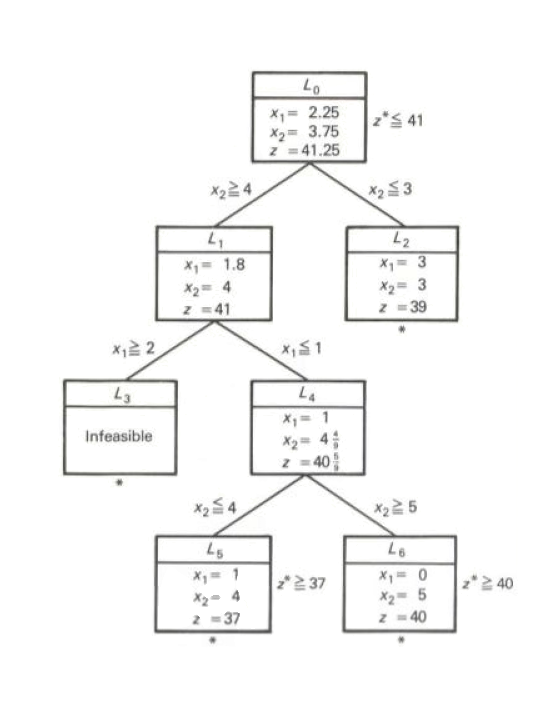
\includegraphics[width=200pt, height=200pt]{bnb_ilp.eps}
%    \caption{B\&B stablo ILP problema.}
%    \label{fig:bnb_ilp}
%\end{figure}

\begin{figure}
	\centering
	\begin{tikzpicture}
		\node[parent node,rectangle split parts=1](A){\textA};
		%\node[parent node,below =of A](B){\textB};
		\node[parent node,below left =of A](B){\textC};
		\node[parent node,below right =of A](C){\textD};
		\node[parent node,node distance=1 and 0.3,below left =of B](D){\textE};
		\node[parent node,node distance=1 and 0.3,below right =of B](E){\textF};
		\node[parent node,node distance=1 and 0.3,below left=of E](G){\textG};
		\node[parent node,node distance=1 and 0.3,below right=of E](H){\textH};
		%\draw[->](A.south)--(B)node[midway,right]{\scriptsize solve as continous problem};
		\draw[->](A.south)--+(0,-0.5)-|(B)node[right,near end]{\scriptsize $x_2\geq 4$};
		\draw[->](A.south)--+(0,-0.5)-|(C)node[left,near end]{\scriptsize $x_2\leq 3$};
		\draw[->](B.south)--+(0,-0.5)-|(D)node[left,near end]{\scriptsize $x_1 \geq 2$};
		\draw[->](B.south)--+(0,-0.5)-|(E)node[right,near end]{\scriptsize $x_1 \leq 1$};
		\draw[->](E.south)--+(0,-0.5)-|(G)node[left,midway]{\scriptsize $x_2\leq 4$};
	    \draw[->](E.south)--+(0,-0.5)-|(H)node[left,midway]{\scriptsize $x_2 \geq 5$};
	\end{tikzpicture}
	\caption{Primjer Branch and Bound  Metoda za ILP.}
	\label{fig:bnb_ilp}
\end{figure}




\subsection{Implicitna Enumeracija}
Posmatrajmo sada specijalnu B\&B proceduru koja se može primijeniti na problem Binarnog cjelobrojnog programiranja. Ovaj algoritam ne zahtjeva da se izvedu rješenja LP-relaksacija, već rad sa kompletnom enumeracijom. Dakle, izlistaju se sve binarne kombinacije za varijable i izabere se ona koja je dpustiva i daje najveću vrijednost ciljnoj funkciji. Ovaj pristup radi dobro na problemima malih dimenzija gdje postoji svega nekoliko binarnih varaijbli u modelu. Primijetimo da u problemu sa $n$ binarnih varijabli imamo broj kombinacija od $2^n$ (dakle, raste eksponencijalnom brzinom). Ideja ove B\&B procedure je u svakom koraku ovog metoda fiksirati neku od varijabli na 0 ili 1, dobijajući dva nova potptoblema koja treba da budu riješena. 

Fiksiramo $i=1$ i $LB=-\infty$. 

\begin{enumerate}
    \item U početnom problemu  $x_j=0$ za sve $j$ (kažemo da je svaka varijabla \emph{slobodna}). Ako je dobijeno rješenje dopustivo, ažuriramo vrijednost u LB.
    \item Fiksiramo $x_i=0$  i $x_i=1$, te dobijamo dva podproblema koja treba riješiti.
    \item  Provjerimo u oba podproblema da li tako fiksirano rješenje dopustivo. U slučaju da jeste, na osnovu koeficijenata u ciljnoj funkciji (pozitivni ili negativni) ako su sve ostali koeficijenti nefiksirani (neslobodnih) varijabli negativni, zaključujemo da je to rješenje najbolje za fiksirane varijable u podproblemu i dalje ne dijelimo više ovaj protproblem. Ako svi takvi koeficijenti nisu negativni, idemo na korak 3. Primijetimo da   podproblem sa fiksnim $x_i=0$ ne mora da provjeravamo, jer je on isti kao i početni (korjeni) problem.
    \item Azuriramo $i = i+1$ i idemo na korak 3 sa podproblemima koji mogu dalje da se dijele, dok god je $i \leq n$. Inače, izlazimo iz petlje sa optimalnim rješenjem (LB). 
\end{enumerate}
 Primijetimo da i u ovom slučaju dobijamo drvo odluke (binarno drvo) gdje su na granama koje spajaju čvor na dubini $i$ sa čvorom na dubini $i+1$  ugrađene odluke da li je varijabla $x_i$ fiksirana na 0 ili 1.

Na Slici~(\ref{fig:bnb_binary}) je dato ovakvo drvo odlučivanja za problem 
\begin{align}
   &\max -8 x_1 - 2x_2 - 4x_3 - 7x_4 -5x_5 + 10 \\
   & -3 x_1 - 3 x_2 + x_3 + 2 x_4 + 3 x_5 \leq -2 \\
   & -5 x_1 - 3 x_2 - 2 x_3 - x_4 + x_5 \leq -4 \\
   & x_i \in \{0, 1\}, \mbox{ za } i=1,\ldots,5.
\end{align}

%\begin{figure}
%    \centering
%    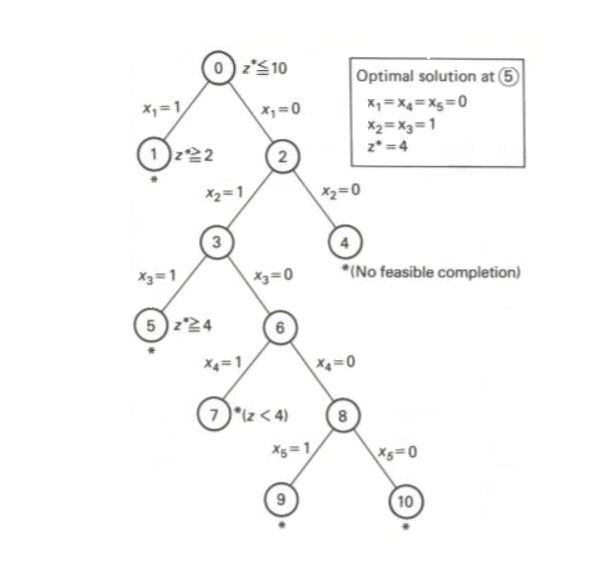
\includegraphics[width=200pt,height=200pt]{bnb_binary.eps}
%    \caption{Drvo odluke za rješavanje problema binarnog programiranja.}
%    \label{fig:bnb_binary1}
%\end{figure}

\begin{figure}
	\centering
\begin{tikzpicture}[
	node/.style={%
		draw,
		circle,
	},
	]
	% nacrtaj cvorove:
	\node [node, label={[blue]right:$z^* \leq 10$}] (A) { 0 };
	\path (A) ++(-135:\nodeDist) node [node, label={[blue]right:$z^* \geq 2$}] (B) {1};
	\path (A) ++(-45:\nodeDist) node [node] (C) {2};
	\path (C) ++(-135:\nodeDist) node [node] (D) {3};
	\path (C) ++(-45:\nodeDist) node [node, label={[blue]right:(Nema dopustivog rješenja)}] (E) {4};
	
	\path (D) ++(-135:\nodeDist) node [node, label={[blue]left:$z^* \geq 4$}] (F) {5};
	\path (D) ++(-45:\nodeDist) node [node] (G) {6};
	
	\path (G) ++(-135:\nodeDist) node [node, label={[blue]right:$z < 4$}] (H) {7};
	\path (G) ++(-45:\nodeDist) node [node] (I) {8};
	
	\path (I) ++(-135:\nodeDist) node [node, label={[blue]left: (Nije dopustivo)}] (K) {9};
	\path (I) ++(-45:\nodeDist) node [node, label={[blue]right: (Nije dopustivo)}] (L) {10};
	% nacrtaj grane:
	\draw (A) -- (B) node [left,pos=0.25] {$x_1=1$}(A);
	\draw (A) -- (C) node [right,pos=0.25] {$x_1=0$}(A);
	\draw (C) -- (D) node [left,pos=0.25] {$x_2=1$}(C);
	\draw (C) -- (E) node [right,pos=0.25] {$x_2=0$}(C);
	
	\draw (D) -- (F) node [left,pos=0.25] {$x_3=1$}(D);
	\draw (D) -- (G) node [right,pos=0.25] {$x_3=0$}(D);
	
    \draw (G) -- (H) node [left,pos=0.25] {$x_4=1$}(G);
	\draw (G) -- (I) node [right,pos=0.25] {$x_4=0$}(G);
	
    \draw (I) -- (K) node [left,pos=0.25] {$x_5=1$}(I);
	\draw (I) -- (L) node [right,pos=0.25] {$x_5=0$}(I);
	
	%add text (info) x1=x4=x5=0; x2=x3=1 je optimum:
	
\end{tikzpicture}
    \caption{Drvo odluke za rješavanje problema binarnog programiranja.}
    \label{fig:bnb_binary}
\end{figure}

Prodiskutujmo ovo rješenje po čvorovima stabla:
  \begin{itemize}
      \item U čvoru 0 imamo da je rješenje $x_i = 0$, za sve $i$ nije dopustivo, ali znamo da je tada $z^*=f(x) \leq 10$.
      \item  Dalje, granamo ovaj problem na dva (korak 2), jedan gdje je $x_i=1$ a drugi $x_1=0$, odakle dobijamo dva podproblema (odgovaraju čvorovima 1 i 2). U čvoru 2 imamo podproblem gdje je fiksiran $x_1=1$. Jasno je da kada uvrstimo ovu vrijednost u početni problem, fukcija cilja nikad neće biti veća od 2 (negativnost koeficijenata funkcije cilja slobodnih varijabli), odakle zaključujemo da je za ovaj podproblem $z^*=f(x) \geq 2$, za sve dopustive vektore $(1,x_2,\ldots,x_n)$. Prema tome, imamo LB=2. 
      \item Problem u čvoru 2 je isti kao problem u čvoru 1, pa nastavljamo dalje sa dijeljenjem problema. 
      \item Sada fiksiramo promjenjivu $x_2$ (uz već fiksiran $x_1 =0$). 
            Za podproblem u čvoru 4, provjerimo da ne postoji dopuna do doustivog rješenja za ovako fiksirane vrijednosti, pa tu stajemo sa njim. Za podproblem u čvoru 3, imamo sada podjelu na dva podproblema fiksirajući varijablu $x_3$, tj. dva odgovarajuća nova čvora 5 i 6. Za problem u čvoru 5, lako se vidi da za ovakve fiksirane varaijble imamo 
            $z^*=f(x) \leq 4$, pa je novo najbolje rješenje LB=4. Problem u čvoru 6 dijelimo dalje (po varijabli $x_4$), podakle dobijamo dva nova podproblema, koji odgovaraju čvoru 7 i 8. Lako se vidi (iz samo jednog dopustivog rješenja) da je $z^*<$LB.  Za čvor 8, imamo novo grananje (po varijabli $x_5$). Kako su ovdje sve varijable kompletno fiksne, primijetimo da niti jedna od ovih tačaka  nije dopustiva.
            \item Prema tome, optimalno rješenje početnog problema je LB=4 i dostiže se u tački $x=(0, 1, 1, 0, 0)$. 
  \end{itemize}
  Napomenimo da se čvorovi čiji je odgovarajući problem podijeljen na podregione se naziva \emph{neaktivan}, a inače \emph{aktivan}. Generalni B\&B metod za rješavanje problema ILP-a je dat   pseudokodom~(\ref{bnb_algorithm_ilp}). 
 
 
 \begin{algorithm}[H] 
\begin{algorithmic}
\WHILE{postoji neki aktivni čvor}
   \STATE  $j \gets$ neka od aktivnih varijabli;
   \STATE  Označiti $j$ kao neaktivnu;
   \STATE  $x^j \gets$ Riješiti podproblem koji odgovara čvoru $j$
   \STATE $z^*_j \gets f(x^j)$;
   \IF{ $z^*_j  \leq$ LB} 
       \STATE Čvor $j$ nije relevantan za dalje razmaranje; 
   \ENDIF
   \IF{$z^*_j  >$ LB}
       \IF{$x^j$ je dopustivo}
            \STATE LB $\gets z^*_j$;
            \STATE $x^* \gets x^j$;
       \ENDIF
   \ENDIF
    \IF{$z^*_j  >$ LB}
       \IF{$x^j$ nije dopustivo}
        \STATE Generisati podprobleme (čvorove) problema koji odgovara problemu čvora $j$ (branch procedura);
        \STATE Označi aktivnim nove čvorove; 
      \ENDIF
   \ENDIF
\ENDWHILE
\end{algorithmic}
\caption{Generalni B\&B za rješavanje ILP-a.}\label{bnb_algorithm_ilp}
\end{algorithm}
 
\emph{Napomene.} Da bi se granice čak i poboljšale, imajmo na umu sljedeće činjenice:
\begin{itemize}
    \item Ako su koeficijenti ciljne funkcije cjelobrojni, onda $z^* \leq \lfloor z^* \rfloor$;
    \item Dodavanjem važećih ograničenja u sam model (fokus sljedećeg poglavlja). 
\end{itemize}
 
\subsection{Metoda Odsjecajućih Ravni}
  
\emph{Metoda Odsjecajućih Ravni} rješava cjelobrojne programe mijenjanjem rješenja linearnog programiranja dok se ne dobije cjelobrojno rješenje. Metoda ne radi  na principu dijeljenja dopustivog regiona problema na podregione, kao u B\&B metodama, već radi sa jednim linearnim programom, koji poboljšava dodavanjem novih ograničenja. Nova ograničenja sukcesivno smanjuju dopustiv region dok se ne pronađe cjelobrojno optimalno rješenje.   
 Istorijski gledano, to je prvi algoritam razvijen za probleme cjelobrojno programiranja za koji se dokazalo da konvergira u konačnom broju
koraka. Generalno, iako se algoritam općenito smatra vrlo neefikasnim, ovaj metod je dovelo do drugih, učinkovitijih algoritama.  
  
\emph{Validna nejednakost} za ILP je svako ograničenje koje ne eliminiše niti jedno moguće cjelobrojno rješenje problema. Drugo ime za nju je \emph{odsjecajuća ravan}.
Recimo ako imamo sljedeći problem ILP-a:
\begin{align*}
    &\max z = 3x_1 + 4 x_2 \\
    &\mbox{pod uslovima } \\
    &5x_1 + 8x_1 \leq 24 \\
    & x_1, x_2 \geq 0, x_1,x_2\in \mathbb{Z}
\end{align*}
validna nejednakost je $z \leq 5$. 

\begin{definition}
      Konveksni omotač je najmanji dopustivi region LP-a koji sadrži sve cjelobrojne tačke problema~(\ref{ilp-formulation}).
\end{definition}
Ako riješimo LP problem čiji je dopustivi skup konveksni omotač cjelobrojnih tačkaka, onda je to rješenje optimalno za odgovarajući ILP. Međutim ovaj problem je poznat kao NP-težak, pa prema tome nije očekivano da se takav konveksni omotač može naći u generalnom slučaju. Nalazak korisnih ograničenja (ne svih) koja učestvuju u izgradnji konveksnog omotača je takođe veoma težak zadatak, mada je ovo ponekad moguće (kao u slučaju problema trgovačkog putnika). Prema tome, ostaje nam naći korisne odsjecajuće ravni neovisno od problema nalaska konveksnog omotača, što je i najčešći slučaj u praksi. 

Pogledajmo sljedeći \emph{problem pakovanja skupa} dat na sljedeći način. Neka je data kolekcija $D$ rombova ( u $\mathbb{R}^2$). 
Zadatak se sastoji od odabira maksimalnog broja rombova tako da se niti jedan od njih ne prepliće.  Za rombove kažemo da se prepliću ako imaju barem jednu zajedničku tačku u presjeku. 
Neka je $O$ skup svih parova rombova koji se prepliću. Sljedeći ILP odgovara ovom problemu:
\begin{align*}
    &\max \sum_{d\in D}x_d\\
    & x_d + x_{d'} \leq 1, \forall (d, d^{'}) \in O \\
    & x_d \in \{0,1\}, \forall d \in D,
\end{align*}
gdje je $x_d$ binaran varijabla koja dobija vrijednost 1 ako je romb $d$ selektovan, inače 0. 
Kao što vidimo, broj binarnih varijabli u praksi može biti veoma velik za ovaj problem, što nas rješava mogućnosti efikasne primjene neke od B\&B tehnika.

Pokušajmo dodati odsjecajuće ravni u prethodni ILP. Za svaku tačku $c$, enumerišimo sve one (moguće) rombove iz $D$ koje sadrže ovu tačku. Označimo takav skup sa $D(c)$. Prema tome, za svaki skup $D(c)$, najviše jedan romb može da budee selektovan. Prema tome, dodajemo sljedeća ograničenja:
\begin{equation}
     \sum_{d \in D(c)} x_d \leq 1, \forall c.
\end{equation}
Ove odsjecajuće ravni će ubrzati rješavanje ovog problema za nekoliko redova veličine.

Pozabavimo se sada \emph{Gomorijevim odsjecajućim ravnima}, geeneralnom metodu za dodavanje odsjecajućih ravni u ILP.  Ideja je dobiti ove ravni iz nekog ograničenja optimalne tabele simpleks metode LP relaksacije. Neka simpleks metod proizvede sljedeći skup jednakosti u formi:

$$x_i + \sum_{ij} \overline{a}_{i,j} w_j= \overline{b}_i, i=1, \ldots,m$$
gdje su $x_i$ bazne promjenjive, a $w_j$ nebazne promjenjive. Napišimo ovu jednakost u drugačijem obliku tako da su na lijevoj strani cjelobrojni dio, dok je na desnoj decimalni dio, tj.
$$x_i + \sum_{ij} \lfloor \overline{a}_{i,j} \rfloor w_j - \lfloor \overline{b}_i \rfloor = \overline{b}_i - \lfloor \overline{b}_i  \rfloor    - \sum_{ij} (\overline{a}_{i,j} - \lfloor \overline{a}_{i,j} \rfloor) w_j.$$

Ako je $x$ dopustivo cjelobrojno rješenje, onda je desna strana manja od 1, pa kako je lijeva strana cjelobrojan u tom slučaju, dobijamo da je ona manja ili jednaka 0, pa imamo
\begin{equation}\label{eq:gomory_cuts}
    \overline{b}_i - \lfloor \overline{b}_i  \rfloor    - \sum_{j} (\overline{a}_{i,j} - \lfloor \overline{a}_{i,j} \rfloor) w_j \leq 0
\end{equation}
za bilo koje dopustiv rješenje koje je cjelobrojno. Dalje, kako su nebazne varijable jednake 0 u bilo kom baznom rješenju, tada imamo 
$$ \overline{b}_i - \lfloor \overline{b}_i  \rfloor    - \sum_{ij} (\overline{a}_{i,j} - \lfloor \overline{a}_{i,j} \rfloor) w_j = \overline{b}_i - \lfloor \overline{b}_i \rfloor  > 0.$$
Prema tome, pokazali smo da odsjecajuće ravni~(\ref{eq:gomory_cuts}) ne odstranjuju bazna dopustiva rješenja, pa ispunjava sve uslove. Uvodeći dodatnu promjenjivu $y_i$ za nejednakosti u (\ref{eq:gomory_cuts}), sljedeća ograničenja dodajemo u LP:
\begin{align}\label{gomory_cplex}
       \overline{b}_i - \lfloor \overline{b}_i \rfloor=   \sum_{j} (\overline{a}_{i,j} - \lfloor \overline{a}_{i,j} \rfloor) w_j - y_i 
\end{align}

\emph{Primjer.} Neka je dat sljedeći ILP problem:\\
$$\begin{array}{ccc}
    & &\max 3 x_1 + 4 x_2 \\
    & \mbox{s.t. } &\frac{2}{5}x_1 + x_2 \leq 3 \\
    & &\frac{2}{5}x_1 - \frac{2}{5}x_2 \leq 1 \\
    & &x_1, x_2 \geq 0, \\
    & & x_1, x_1 \in \mathbb{Z}.
\end{array}$$
Riješimo ga uz pomoć gomorijevih odsjecajućih ravni. 

\emph{Rješenje.}
Prva simpleks tabela je 

$$\begin{array}{cccc|c}
   \frac{2}{5}           & 1               & 1 & 0 & 3 \\
   \frac{2}{5}           & -\frac{2}{5}    & 0 & 1 & 1 \\ \hline
   -3                    &  -4             & 0 & 0 & 0
\end{array}$$
Dovedimo drugu varijablu (kolona 2) u bazu, pa imamo 
$$\begin{array}{cccc|c}
   \frac{2}{5}           & 1               & 1           & 0 & 3 \\
   \frac{14}{25}         & 0               & \frac{2}{5} & 1 & \frac{11}{5}\\ \hline
   -\frac{7}{5}                  & 0               &4 & 0 & 12
\end{array}$$
Dalje, biramo pivot element u datoj simpleks tabeli, a to je elemet $\overline{a}_{2,1} = \frac{14}{25}$, pa dobijemo simpleks tabelu
$$
\begin{array}{cccc|c}
    0    &  1  &  \frac{10}{14} &  -\frac{10}{14}  &  \frac{20}{14}                  \\
    1    &  0  &  \frac{10}{14} &   \frac{25}{14}  &   \frac{55}{14}\\ \hline
    0    &  0  &  5             &    \frac{5}{2}   &    \frac{35}{2}
\end{array}
$$
Kako u posljednjoj vrsti nemamo negativnih vrijednosti, zaključujemo da je ovo optimalna simpleks tabela. Na osnovu (\ref{gomory_cplex}),   za prvi red simpleks tabele i odrogarajuće ogranjičenje generišemo odsjecajuću ravan:
$$   \frac{5}{7}x_3 + \frac{2}{7} x_4 +      y_1   = \frac{6}{14}=\frac{3}{7}$$
pa je dodajemo u (završnu) simpleks tabelu:
$$
\begin{array}{ccccc|c}
    0    &  1  &  \frac{10}{14} &  -\frac{10}{14}  &  0 & \frac{20}{14}                  \\
    1    &  0  &  \frac{10}{14} &   \frac{25}{14}  &  0 & \frac{55}{14}\\ 
    0    &  0  & \frac{5}{7}    &   \frac{2}{7}    &  -1 & \frac{3}{7}  \\
     \hline 
    0    &  0  &  5             &    \frac{5}{2}   &  0 &    \frac{35}{2}
\end{array}
$$
Načinimo sada jediničnu podmatricu u gornjoj lijevoj matrici $\overline{A}$, za treću kolonu (i odgovarajuću varijablu $x_3$), pivotirajući oko elementa $\overline{a}_{3,3}$, čime dobijamo 

$$
\begin{array}{ccccc|c}
    0    &  1  &   0 &   -1  &            1 & 1                  \\
    1    &  0  &  0 &    \frac{3}{2}  &  1 & \frac{7}{2}\\ 
    0    &  0  &  1  &   \frac{2}{5}    &  -\frac{7}{5} & \frac{3}{5}  \\
     \hline 
    0    &  0  &  0   &    \frac{1}{2}  &  7  &    \frac{29}{2}
\end{array}
$$
Kao što vidimo, rješenje problema je $(\frac{7}{2}, 1, 0, 0, \frac{3}{5})$, što i dalje nije cjeloborjno rješenje. Dalje, dodajemo novu odsjecajuću ravan, koja se izvodi iz drugog ograničenja (drugi red simpleks tabele): 
$$ \frac{1}{2} x_4 - y_2 = \frac{1}{2}.$$
Dodajmo ovo ograničenje u posljednju simpleks tabelu:

$$
\begin{array}{cccccc|c}
    0    &  1  &   0 &   -1  &            1 & 0 & 1                  \\
    1    &  0  &  0 &    \frac{3}{2}    &  1 & 0 &  \frac{7}{2}\\ 
    0    &  0  &  1  &   \frac{2}{5}    &  -\frac{7}{5} &  0 & \frac{3}{5}  \\
    0    & 0   &  0  &   \frac{1}{2}    & 0     & -1 & \frac{1}{2} \\
     \hline 
    0    &  0  &  0   &    \frac{1}{2}  &  7  &   0 &  \frac{29}{2}
\end{array}
$$
Sada za varijablu $x_4$ (četvrta kolona), pivotiramo oko elementa $\overline{a}_{4,4}$, pa dobijamo simpleks tabelu 

$$
\begin{array}{cccccc|c}
0 &  1   &  0  &  0  &    1             &    -2           &   2         \\
1 &  0   &  0  &  0  &    1             &     3           &   2         \\
0 &  0   &  1  &  0  &   -\frac{7}{5}   &     \frac{4}{5} &   \frac{1}{5}\\
0 &  0   &  0  &  1  &   0              &    -2           &   1   \\ \hline
0 &  0   &  0  &  0  &   7              &     1           &   14
\end{array}
$$


Iz tabele zaključujemo da je bazno rješenje problema 
$x=(2,2, \frac{1}{5}), 1)$, a optimalno $(2, 2)$, što je i optimalno rješenje početnog problema. 

Rješenje ILP problema gdje su svi koeficijenti u ograničenjima cjelobrojni, je prikazano sljedećim primjerom.
%https://www.math10.com/en/geometry/geogebra/geogebra.html
\emph{Primjer}. Riješimo sljedeći problem ILP-a:
\begin{align*}
    &\max 3 x_1 + 4 x_2 \\
    &\mbox{s.t.} \\
    & 3 x_1 - x_2 \leq 12 \\
    & 3 x_1 + 11 x_2 \leq 66 \\
    & x_1, x_2 \geq 0 \\
    & x_1, x_2 \in \mathbb{Z}
\end{align*}
\emph{Rješenje. }
Na Slici~(\ref{fig:region_ilp_primjer_2}), dat je skup tačaka koje su dopustive za problem, kao i optimalna tačka $x=(5,4)$.
\begin{figure}
    \centering
    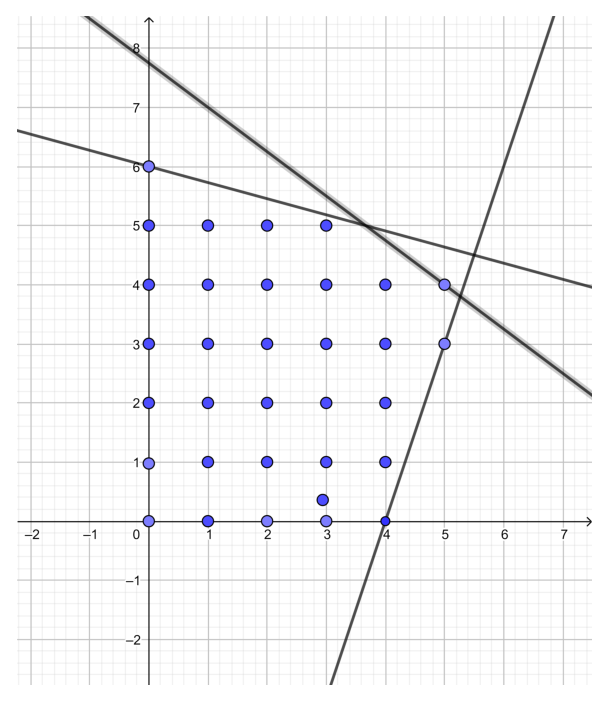
\includegraphics[width=170pt,height=170pt]{region_ilp_primjer_2.eps}
    \caption{Dopustiv skup tačaka problema.}
    \label{fig:region_ilp_primjer_2}
\end{figure}

Riješimo sada ovaj problem uz pomoć Gomorijevih odsjecajućih ravni. 
Početna simpleks tabela je data sa 
$$\begin{array}{ccc c| c}
    3  & -1 & 1 &  0  & 12  \\
    3  & 11 & 0 &  1  & 66 \\ \hline
   -3  & -4 & 0 &  0  & 0
\end{array}$$
Nakon dvije iteracije pivotiranja, dobijamo simpleks tabelu 
$$\begin{array}{ccc c| c}
1 & 0 &  \frac{11}{36}   &  \frac{1}{36}  &  \frac{11}{2} \\
0 & 1 &  -\frac{1}{12}  &  \frac{1}{12}  &  \frac{9}{2}   \\ \hline
0 & 0 &  \frac{7}{12}   &  \frac{5}{12}  &  \frac{69}{2}
\end{array} $$
Optimalno rješenje je $x^* = (\frac{11}{2}, \frac{9}{2}, 0, 0)$ koje nije cjelobrojno. Dodajmo gomorijevu otsjecajuću ravan generisanu iz ograničenja u prvoj vrsti simpleks tabele (za prvu baznu komponentu $x_1^* = \frac{11}{2}$):
$$  \frac{11}{36} x_2 + \frac{1}{36} x_3 - y_1 = \frac{1}{2},$$
pa dobijamo tabelu 
$$\begin{array}{ccccc| c}
1 &  0 &   \frac{11}{36}  & \frac{1}{36}   &  0 & \frac{11}{2} \\
0 &  1 &   -\frac{1}{12}  & \frac{1}{12}   &  0 & \frac{9}{2} \\
0 &  0 &  \frac{11}{36}   &  \frac{1}{36}  & -1 & \frac{1}{2} \\ \hline
0 & 0  &  \frac{7}{12}    & \frac{5}{12}   &  0 & \frac{69}{2}
\end{array} $$
Kako bazno dopustivo rješenje nije očigledno, primijenimo dvofazni simpleks metod da bi izabrali bazu, odakle dobijamo tabelu 
$$\begin{array}{ccccc| c}
1   &   0       &   0   &   0             & 1              & 5 \\
0   &   1       &   0   &   \frac{1}{11}  & -\frac{3}{11}  & \frac{51}{11} \\
0   &   0       &   1   &   \frac{1}{11}  & -\frac{36}{11} &  \frac{18}{11} \\ \hline
0   &   0       &   0   &   \frac{4}{11}  & \frac{21}{11}  &  \frac{369}{11} \\
\end{array} $$
Kako su svi koeficijenti u posljednjoj vrsti veći od 0, slijedi da je optimalno bazno rješenje jednako $x=(5, \frac{51}{11}, \frac{18}{11}, 0, 0)$, koje opet nije cjelobrojno. 
 Prema tome, dodajmo sljedeću gomorijevu odsjecajuću ravan za bazno rješenje $x^*_2 = \frac{51}{11}$ (posmatrajući vrstu 2 posljednje simpleks tabele):
 
 $$ \frac{1}{11} x_4 + \frac{8}{11} x_5 - y_2 = \frac{11}{18},$$
 odakle imamo tabelu 
 $$\begin{array}{cccccc| c}
 1   &   0   &  0  &   0             &   1  &   0              &   5 \\
 0   &   1   &  0  &  \frac{1}{11}    &   -\frac{3}{11}    &  0 & \frac{51}{11} \\
 0   &   0   &  1  &  \frac{1}{11}    & -\frac{36}{11}       & 0 & \frac{18}{11}  \\
 0   &   0   &  0  &  \frac{1}{11}    &  \frac{8}{11}   & -1 & \frac{7}{11} \\ \hline
 0   &   0   &  0  &   \frac{4}{11}   &   \frac{21}{11} & 0 & \frac{369}{11}
\end{array} $$
I dalje nije očigledno šta su bazne varijable, pa uradimo dvofazni simpleks metod, te dobijamo 
 $$\begin{array}{cccccc| c}
1    &   0   &   0   &  -\frac{1}{8}   &   0    &    \frac{11}{8}    &  \frac{33}{8} \\
0    &   1   &   0   &   \frac{1}{8}   &   0    &    -\frac{3}{8}    & \frac{39}{8} \\
0    &   0   &   1   &   \frac{1}{2}   &   0    &    - \frac{9}{2}   & \frac{9}{2} \\
0    &   0   &   0   &   \frac{1}{8}   &   1    &    - \frac{11}{8}  & \frac{7}{8} \\ \hline
0    &   0   &   0   &   \frac{1}{8}   &   0    &     \frac{21}{8}   & \frac{255}{8}
\end{array} $$
Odgovarajuće optimalno bazno dopustivo rješenje i dalje nije cjelobrojno -- niti jedna komponenta nije cjelobrojna. 

Prema tome, dodajemo gomorijevu odsjecajuću ravan za vrstu 2 prethodne simpleks tabele, koja je oblika
$$  \frac{1}{8}x_4 + \frac{5}{8} y_2 - y_3 = \frac{7}{8},$$
te dobijamo tabelu
$$ \begin{array}{ccccccc| c}
1    &   0   &   0   &  -\frac{1}{8}   &   0    &    \frac{11}{8}    & 0 & \frac{33}{8} \\
0    &   1   &   0   &   \frac{1}{8}   &   0    &    -\frac{3}{8}    & 0 & \frac{39}{8} \\
0    &   0   &   1   &   \frac{1}{2}   &   0    &    - \frac{9}{2}   & 0 & \frac{9}{2} \\
0    &   0   &   0   &   \frac{1}{8}   &   1    &    - \frac{11}{8}  & 0    & \frac{7}{8} \\ 
0    &   0   &   0   &   \frac{1}{8}   &   0    &    \frac{5}{8}   & -1 & \frac{7}{8} \\ \hline
0    &   0   &   0   &   \frac{1}{8}   &   0    &     \frac{21}{8}   & 0 & \frac{255}{8}   
\end{array} $$
I dalje nije jasno koju još varijablu treba dodati u bazne varijable (bazu), uradimo dvofazni simpleks metod, odakle dobijamo 

$$ \begin{array}{ccccccc| c}
    1    &   0   &   0   &  0 &  1  &   0    &    0    & 5  \\
0    &   1   &   0   &  0   &   -\frac{1}{2}    &   0   & \frac{1}{2} & 4 \\
0    &   0   &   1   &  0   &   -\frac{7}{2}    &   0   & \frac{1}{2} & 1 \\
0    &   0   &   0   &  1  &   \frac{5}{2}    &  0 &  -\frac{11}{2}    & 7 \\ 
0    &   0   &   0   &   0 &  -\frac{1}{2}    &   1   & - \frac{1}{2} & 0\\ \hline
0    &   0   &   0   &  0  &   1    &    0   & 2 & 31  
\end{array} 
$$
gdje je lako uočiti da je optimalno bazno dopustivo rješenje $x=(5, 4, 1, 7, 0, 0, 0 )$, tj. rješenje početnog problema je $x^*=(5, 4)$.

\subsection{B\&C algoritam za rješavanje ILP-a}
%https://homepages.rpi.edu/~mitchj/handouts/bc_algo/
% http://www.mi.fu-berlin.de/wiki/pub/Main/GunnarKlauP1winter0708/discMath_klau_ILP_I.pdf
Za razliku od B\&B procedure koja rješava ILP, ovdje dodajemo i metod odsjecajućih ravni u rješavanju relaksacija podproblema koji odgovaraju čvorovima (drveta). Dakle, ako  uzimamo trenutno aktivni čvor i rješavamo njegov podproblem, dijelimo ga na nekoliko podproblema (podjelom dopustivog regiona na više disjunktnih -- dodavanjem ograničenja) pa takve probleme rješavamo rekurzivnim dodavanjem (gomorijevih) odsjecajućih ravni. Primijenimo ovu ideju na rješavanje jednog ILP-a.

\emph{Primjer}.  Riješimo problem modelovan uz pomoć sljedećeg ILP-a:
\begin{align*}
    &\max 6 x_1 + 5 x_2 \\
    & \mbox{s.t. } \\
    & 3x_1 + x_2 \leq 11 \\
    & - x_2 + 2 x_2 \leq 5 \\
    & x_1, x_2 \geq 0 \\
    & x_1, x_1 \in \mathbb{Z}
\end{align*}

\emph{Rješenje}. B\&C procedura prvo rješava LP relaksaciju početnog problema (simpleks metodom), odakle dobijamo rješenje $x=(\frac{17}{7}, \frac{26}{7})$
sa optimalnom vrijednošću $33\frac{1}{7}$. Nakon toga treba da se donese odluka, da li se problem rješava dodavanjem odsejcajućih ravni ili podjelom dopustivog regiona na manje (disjunktne) podregione. Podijelimo region po koordinati $x_1$, odakle ćemo dobiti dva podproblema 

\begin{align*}
    &\max 6 x_1 + 5 x_2 \\
    & \mbox{s.t. } \\
    & 3x_1 + x_2 \leq 11 \\
    & - x_2 + 2 x_2 \leq 5 \hspace{2cm} (P1) \\
    & x_1 \geq 3 \\
    & x_2 \geq 0 \\
    & x_1, x_2 \in \mathbb{Z}
\end{align*}

\begin{align*}
    &\max 6 x_1 + 5 x_2 \\
    & \mbox{s.t. } \\
    & 3x_1 + x_2 \leq 11 \\
    & - x_2 + 2 x_2 \leq 5 \hspace{2cm} (P2) \\
    & x_1  \leq 2 \\
    & x_2 \geq 0 \\
    & x_1, x_2 \in \mathbb{Z}
\end{align*}

Relaksacija problem ($P1$) daje riješenje $x^*=(3,2)$, koje je cjelobrojno, pa prema tope i dopustivo u početnom problemu. Njena vrijednost je 28, što je i donja granica (LB) početnog problema. Relaksacija problema ($P2$) nam daje rješenje $x^*=(2, \frac{7}{2})$, čija je optimalna vrijednost $\frac{29}{2}$.  Prema tome, rješenje nije cjelobrojno. Primjenjujući metod odsjecajućih ravni, dobijamo da je potrebno dodati ograničenje $2x_1 + x_2 \leq 7$ u problem ($P2$) pa dobijamo problem 
\begin{align*}
     &\max 6 x_1 + 5 x_2 \\
    & \mbox{s.t. } \\
    & 3x_1 + x_2 \leq 11 \\
    & - x_2 + 2 x_2 \leq 5  \\
    & 2x_1 + x_2 \leq 7 \hspace{2cm} (P3)\\ 
    & x_1  \leq 2 \\
    & x_2 \geq 0 \\
    & x_1, x_2 \in \mathbb{Z}
\end{align*}

Rješavajući LP relaksaciju problema ($P3$), dobijamo rješenje $x^*=(\frac{9}{5}, \frac{17}{5})$, tj.  optimalna vrijednost je $27.8$. Kako je $LB \geq 28.8$, niti jedno cjelobrojno rješenje problema ($P3$) ne može dostići trenutno najbolju donju granicu (LB=28), pa zaključujemo da je optimalo rješenje početnog problema $x^*=(3,2)$. 

\subsection{Lagranžova relaksacija}
U rješavanju problema optimizacije, garancije da je nađeno rješenje optimalno je jedan od glavnih ciljeva. Međutim, za mnoge probleme nije realno očekivati da se garantuje optimalnost, već najbolje što se može učiniti je da se ponudi dobra dolja granica za optimum. Ako je ta ganica blizu optimuma, u mnogo slučajeva može da zamijeni optimum, a da uštedi vrijeme i resurse. 

Ideja \emph{Lagranžove relaksacije} je da u modelu ILP-a   koji ima  ograničenja koja čine problem teškim (ovo je najčešće stvar praktičnog iskustva),  posmatramo kao dio ciljne funkcije i da je penalizujemo.  %parametrom $\lambda>0$. 
Ovo ograničenje potom brišemo iz skupa ograničenja modela. Na ovaj način, dobija se donja granica (za problem minimizacije) za optimalno rješenje datog problema. U praksi, ovo je često jako blizu optimalnom rješenju. 

\emph{Primjer}. Posmatrajmo problem \emph{najkraćeg puta sa ogaraničenjem} (eng. Constrained Shortest Path Problem). Neka je dat usmjeren neciklifan graf $G=(V,E)$. Za svaku granu $(i,j) \in E$ dodijelimo cijenu puta $c_{i,j}$ i vrijeme putovanja $t_{i,j}$. Pretpostavimo da je čvor $i=1$ startni čvor (izvor), a čvor $n = |V|$ je završni čvor (ušće). Zadatak je da se naće put koji je najeftiniji od izvora do ušća tako da se čitav put pređe u vremenskom periodu $T$.

Modelujemo ovaj problem modelom ILP-a:
 \begin{align}
    &z^*=\min\sum_{(i,j) \in E }c_{i,j}x_{i,j} \\
    &\mbox{s.t. }\\
    & \sum_{i} x_{i,j} - \sum_{i} x_{j,i} = \begin{cases}  
                                               1, \mbox{ ako } i=1 \\
                                              -1, \mbox{ ako } i=n \\
                                               0, \mbox{ inače }
                                            \end{cases} \\
    & \sum_{(i,j) \in E} t_{i,j} x_{i,j} \leq T \\
    & x_{i,j} \in \{0, 1 \}, \forall (i,j) \in E.
\end{align} 

Binarna varijabla $x_{i,j}$ dobija vrijednost 1 ako je odabrana grana $(i,j)$ na   putu, a 0 inače.  
Prvo ograničenje u modelu nam ograničava da je rješenje put od izvora da ušća. Drugo ograničenje nam kazuje da je vrijeme prelaska puta u granicama dopustivog. Ovo ograničenje spada pod ``komplikovanim'' jer, kao što znamo,  pronalazak najkraćeg puta u direktnim grafovima sa izvor čvorom je polinomijalno rješiv (Dajkstrin algoritam), dok uz ograničenje o vremenu taj problem postaje NP-težak problem. Ideja je sada relaksirati ovaj problem uz 
prebacivanje ograničenja o vremenu i penalizirati vrijeme u ciljnoj funkciji. 
Dakle, Lagranžova relaksacija problema je data sa:

\begin{align*}
       &L(\lambda)= \min\sum_{(i,j) \in E }c_{i,j}x_{i,j}  + \lambda(\sum_{(i,j) \in E} t_{i,j} x_{i,j} - T ) = \min \sum_{(i,j) \in E} (c_{i,j} + t_{i,j} )x_{i,j} - \lambda T \\
        &\mbox{s.t. }\\
    & \sum_{i} x_{i,j} - \sum_{i} x_{j,i} = \begin{cases}  
                                               1, \mbox{ ako } i=1 \\
                                              -1, \mbox{ ako } i=n \\
                                               0, \mbox{ inače }
                                            \end{cases} \\
     & x_{i,j} \in \{0, 1 \}, \forall (i,j) \in E.
\end{align*}
Primijetimo da je $L(\lambda) \leq z(\lambda)  \leq z^*$, za sve $\lambda > 0$, gdje je $z(\lambda)$ problem koji ima funkciju cilja $L(\lambda)$ uz uključeno ograničenje o vremenu u skup ograničenja modela. Dakle, za $\lambda$, $L(\lambda)$ nam daje donje ograničenje optimalnog rješenje ovog problema. 

Problem $L^* = \max \{ L(\lambda) \mid \lambda > 0  \}$ se naziva \emph{problem lagranžovog multiplikatora}. Može se pokazati da vrijedi 
$$ L(\lambda) \leq L^* \leq z^*.$$

U praksi se pokazalo da je Lagranžova relaksacija dobra tehnika za dobijanje granica za optimalnu vrijednost problema. Pokušajmo sada primijeniti ovu tehniku na problem trgovačkog putnika. 

Pogledajmo ovaj problem sa grafovske strane. Znamo da kolekcija grana formira rutu ako su svaka dva čvora pokrivena sa dvije grane. Takođe, ako obrišemo grane incidentne sa čvorom 1, ostatak rute čini stablo koje pokriva graf  $G\setminus \{1\}$.  
Definišimo sa $A(j)$ skup svih čvorova koji su incidentni sa čvorom $j$. Relaksacija: definišimo sa $T_1$ skup svih ruta koje nakon brisanja grana koje pokrivaju čvor $1$ formiraju drvo.  

Definišimo model
\begin{align*}
    &z^* = \min \sum_{(i,j)\in E} c_{i,j} x_{i,j}\\
    & \sum_{ \{ i \mid (i,j) \in E \} } x_{i,j} = 2, \forall i \in \{1,\ldots, n \} \\
    & x \in T_1,
\end{align*}
gdje $x_{i,j} = 1$ ako grana $(i,j)$ pripada ruti, a 0 inače.

Lagranžova relaksacija za ovaj problem može se zadati sa 
\begin{align*}
     &L(\lambda) = \min \sum_{(i,j)\in E} c^\lambda_{i,j} x_{i,j} - 2 \sum_{i} \lambda_i \\
     & x \in T_1
\end{align*}
gdje je $\lambda=(\lambda_1, \ldots, \lambda_n)$ i $c^\lambda_{i,j} = c_{i,j} + \lambda_i + \lambda_j$. 

Rješenje problema lagranžovog multiplikatora u praksi daje izvrsna rješenja i obično je blizu prave rute. Optimalno pokrivajuće stablo lagranžovog problema $L(\lambda^*)$ za optimalni $\lambda^*$ obično ima nekoliko visećih čvorova. 

Konstruišimo još jednu Lagranžovu relaksaciju za ovaj problem uvodeći ograničenje pokrivanja, tj. da u svakoj ruti broj grana koje imaju oba kraja u skupu čvorova $S$ kardinalnosti $|S|$ je najviše $|S|-1$, pa imamo: 

\begin{align*}
     & z^* = \min \sum_{(i,j)\in E} c_{i,j} x_{i,j} \\
     & \sum_{ \{ i \mid (i,j) \in E \} } x_{i,j} = 2, \forall i \in \{1,\ldots, n \} \\
     & \sum_{(i,j) \in E} x_{i,j} \leq |S|-1, \forall S \in V \\
     & x_{i,j} \in \{0, 1 \}, (i,j)\in E.
\end{align*}
Lagranživa relaksacija prethodnog ILP-a ima oblik 
\begin{align*}
 &L(\lambda) = \min \sum_{(i,j)\in E} c^\lambda_{i,j} x_{i,j} - 2 \sum_{i} \lambda_i \\
 & \sum_{(i,j) \in E} x_{i,j} \leq |S|-1, \forall S \in V \\
 & \sum_{(i,j) \in E} x_{i,j} = n
\end{align*}
gdje je $\lambda=(\lambda_1, \ldots, \lambda_n)$ i $c^\lambda_{i,j} = c_{i,j} + \lambda_i + \lambda_j$. 

% interior point method (dodati)...
\subsection{Metod Generisanja Kolona}% ovo je za LP probleme sa velikim brojem kolona, pogledati u https://coral.ise.lehigh.edu/~ted/files/ie418/lectures/Lecture18.pdf file:///C:/Users/PC/Downloads/ColumnGenerationTutorial.pdf
Često se u praksi može susresti da je u LP-u (ili ILP-u) broj varijabli puno veći (eksponencijalno) u odnosu na broj ograničenja. U osnovi, riječ je o ekstremno velikim modelima gdje je matrica $A$ velikih dimenzija. Kada je riječ o rješavanju, veliki dio matrice (tj. njene kolone) nam nikada i neće biti relevantan u rješavanju. Da bi se riješila specifična instanca problema, ono što nam je potrebno su:
\begin{itemize}
    \item Ograničenja koja se vežu uz optimalnost.
    \item Varijable koje su bazne u optimalnom rješenju.
\end{itemize}
Prema tome, ono što je potrebno su ograničenja koja imaju pozitivne dualne vrijednosti, kao i varijable koje su pozitivne vrijednosti za optimalnost (vektor doprinosa $\overline{c}$). Ako bismo imali ove varijable i ograničenja od početka, problem bi riješili veoma brzo. Međutim, ova informacija nam nije dostupna.  U simpleks metodi, vektor doprinosa je potrebno računati u svakoj iteraciji, što nije efikasno ako je matrica $A$ velikih dimenzija. Takođe, vrijeme potrebno za generisanje simpleks tabele bi bilo ogromno u tom slučaju.  Oba ova problema su rješiva uz pomoć \emph{pristupa generisanjem kolona}.  Ideja ovog metoda se sastoji u sljedećem:
\begin{itemize}
    \item Krenimo sa ``obećavajućim'' podskupom $S$ kolona matrice $A$; 
    \item Riješimo LP na podskupu kolona $S$; 
    \item Procijenimo ostale kolone i dodajmo u $S$ one sa negativnim 
          cijenama doprinosa;
    \item Itrerativno pozivamo perthodna dva koraka dok god postoje kolone   sa negativnim doprinosom koje nisu u $S$.
\end{itemize}
Tehnički zapisano, krećemo od \emph{restrikovanog problema}
\begin{align*}
    &\min c^T x \\
    &\mbox{s.t} \\
    & \sum_{i \in I} A_i x_i  \leq b \hspace{2cm} (R)\\
    & x \geq 0. 
\end{align*}
kojeg riješimo, te izračunamo optimalno dualno rješenje. Sada je potrebno izgenerisati novu kolonu $A_j$ pri čemu je $c_j - c_B^T B^{-1}A_j < 0$.

Ovo se može uraditi rješavanjem \emph{podproblema}:
$$\min_{a \in C} c_a - c_B^T B^{-1} a,$$
gdje je $C$ globalni skup kolona. 

Ako je rješenje problema kolona $a \in C$ čija je vrijednost strogo manja od 0, dodamo kolonu u skup $S$, te riješimo \emph{restrikovani problem} na novom skupu kolona. Ovaj metod se još naziva \emph{generički metod generisanja kolona}.  
Postoji mnogo pristupa kako ažurirati skup $S$ tokom iteracija. 
Najjednostavniji se tiče zadržavanja svake kolone koja je do sada izgenerisana i dodana u skup $S$. Naprednija strategija se tiče izbacivanja onih kolona iz skupa $S$ koje su nebazne u svakoj iteraciji. 
 U nastavku dajemo primjer primjene \emph{metoda generisanja kolona} na poznatim \emph{ Cutting Stock} problemu. 
 
 \emph{Problem}. Tvornica papira proizvodi role papira fiksne širine  $W$. 
 Kupci naručuju različit broj roli različite širine $W \in \mathbb{R}^m$, dok je sa vektorom $b \in \mathbb{R}^m$ dat zahtjev (broj rolni).  Zadatak je pronaći optimalan način Kako rezati role i smanjiti otpad.  
 
 \emph{Rješenje.} Na Slici~(\ref{fig:cuting_stock_solutions}) je dato rješenje jedne instance problema. 
 Što se tiče kolona za ovom problemu, one predstavljaju dopustive obrasce (kombinacije rezanja). Jedan dio obrasca sa slike, bi bio $1820$ x $2$ (rolne) u prvoj koloni.
 Primijetimo da broj različitih obrazaca raste eksponencijalno u odnosu na broj narudžbi.  Ako bismo enumerisali sve obrasce, trebali bi riješiti sljedeće ILP modele:
 \begin{align*}
      & \min \sum_{i} x_i \\
      & \sum_{ij} a_{i,j }x_j \geq b_i, \forall i \hspace{2cm} (CSILP)\\
      &  x_j \geq 0, x_{j} \in \mathbb{Z} 
 \end{align*}
 gdje je $a_{i,j}$ broj puta da se narudžba $i$ pojavi u obrascu $j$ (vrsta na slici), dok  je $x_j$ broj puta gdje je obrazac $j$ korišten. Primjera radi, na  Slici~(\ref{fig:cuting_stock_solutions}) bi bilo $a_{1,1}=3$ i $x_1 = 2$, dok je $a_{1,2}=0$; $a_{1,5}=1$ i $ x_5 = 12$.
 
 Ideja je ne stvarati obrasce na početku, već ih generisati prema potrebi (po kolonama) koristeći \emph{metod generisanja kolona}. Kolona $a$ odgovara dopustovom obrascu akko vrijedi 
 $$ \sum_{i=1}^m a_i W_i \leq W $$
 gdje $a$ sadrži samo nenegativne (cjelobrojne) vrijednosti. 
% Primijetimo da je cijena svakog paterna po kolonama jednaka za svaku kolonu. 
Primijetimo da je na osnovu prethodnog (razmatrajući relaksaciju problema (CSILP)), vrijednosti koeficijenata doprinosa 
su $\overline{c} = 1 - \sum_{i} A_{j,i} y_i$.  
 Dakle, podproblem izgleda ovako:
 \begin{align*}
     &\max \sum_{i=1}^m y_i a_i \\
     &  \sum_{i} W_i a_i \leq W \hspace{2cm} (CGP)\\
     & a_i \geq 0 \\
     & a_i \in \mathbb{Z},
 \end{align*}
  gdje su $y_i$ vrijednosti optimuma duala. 
 Ovaj problem je poznat pod nazivom \emph{cjelobrojni problem ruksaka} (eng. integer knapsack problem). Iako je NP-težak, ovaj problem se u praksi rješava na vrlo efikasan način uz pomoć dinamičkog programiranja. 
 
 \begin{figure}[!ht]
     \centering
     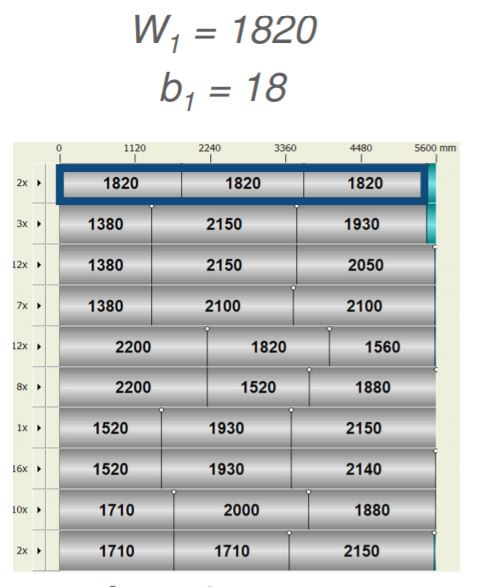
\includegraphics[width=200pt, height=200pt]{cutting_stock.jpg}
     \caption{Rješenje jedne instance (treba nacrtati sliku).}
     \label{fig:cuting_stock_solutions}
 \end{figure}
 Za ovaj problem je lako naći inicijalno bazno dopustivo rješenje:
 za $i$-tu baznu kolonu uzimamo $i$-ti jedinični vektor, tj. obrazac dobijen rezanjem jedne rolne dužine $W_i$. Ovakav skup kolona formira inicijalnu dopustivu bazu. Svakako, malo je vjerovatno da će ove kolone biti korištene u optimalnom rješenju. 
 Prema tome, algoritam za ovaj problem bi išao ovako:
 \begin{enumerate}
     \item Konstruišimo inicijalno bazno dopustivo rješenje (jedinični vektori) i kolone ubacimo u skup $S$.
     \item Riješimo restrikovanu relaksaciju problema ($CSILP$) i vratimo dualno optimalno rješenje. 
     \item Riješimo ($CGP$).
     \item Ako je vrijednost optimalno rješenja negativna, ubaciti novu kolonu (koja je rješenje podproblema) u skup $S$. Inače, prekidamo proces jer je optimalno rješenje nađeno. 
     \item Riješiti LP na novom skupu $S$.
 \end{enumerate}
 Primijetimo da je dodavanje nove kolone u $S$ odgovara dodavanju novog obrasca (u rješenje). 
 
 %Za uraditi: https://ocw.mit.edu/courses/sloan-school-of-management/15-083j-integer-programming-and-combinatorial-optimization-fall-2009/lecture-notes/ (Lekcija 19-25)
 
 \newpage
 
 \section{Dekompozicioni Metodi}
 
 \subsection{Benderova Dekompozicija}
 
  \subsection{Lagranžova Dekompozicija}
 
 \section{Metodi za Nalaženje Dopustivih Rješenja}

\subsection{Pohlepni Algoritmi}

\subsection{Aproksimativni Algoritmi}
  
\subsection{Heuristički Metodi}
 
 \section{Optimizacioni rješavač Cplex}
\end{document}

